
%% Compile with: lualatex presentation.tex
%% Required fonts: Roboto Slab, Fi mra Sans (available on Google Fonts)
\documentclass[aspectratio=169, 12pt]{beamer}

% set your preferred theme
\usetheme{GruvboxWhite}
% Set accent color to aqua
\colorlet{gbAccentColor}{gbAqua}
\usepackage{booktabs}
% nel preambolo, se non già presente
\usepackage{adjustbox}
\usepackage{array}
\usepackage{fontawesome5}
\usetikzlibrary{arrows.meta, positioning} 
\addbibresource{bibliography.bib}

\title{Designing Interactive XR Environments}
\subtitle{Safety, Engagement, and Task Effectiveness Across Immersive and Non-Immersive Systems}
\author[M. Pizzo]{Marianna Pizzo}
\institute{University of Genoa · DIBRIS}
\date{July 10, 2026}

% Custom command for citation footer
\newcommand{\citefooter}[1]{\hfill{\tiny #1}}

\begin{document}

%% ══════════════════════════════════════════════════════════════════════════════
%% PART 1: INTRODUCTION & CONTEXT (6 SLIDES)
%% ══════════════════════════════════════════════════════════════════════════════

\begin{frame}[plain]
	\titlepage
	
	\vspace{0.5cm}
	
	\begin{center}
		\small
		\textbf{Advisors:} Manuela Chessa, Fabio Solari
		
		\textbf{External Reviewers:} Pablo Cesar, Giacinto Barresi
	\end{center}
	
	\begin{tikzpicture}[remember picture, overlay]
		\node[anchor=south east, xshift=-0.4cm, yshift=0.3cm] at (current page.south east) {
			
\includegraphics[height=1cm]{figures/unige.png}
		};
	\end{tikzpicture}

	\vspace{0.2cm}
		
		\small
		PhD Program in Computer Science, XXXVIII Cycle
\end{frame}

\begin{frame}{eXtended Reality: Definition and Scope}
	\small
\textbf{XR} encompasses Virtual Reality (VR), Augmented Reality (AR), and Mixed Reality (MR)
	
	\begin{center}
		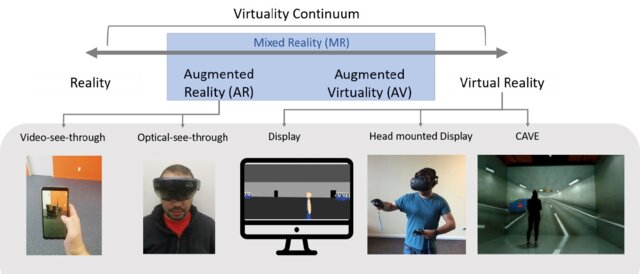
\includegraphics[height=0.37\textheight,keepaspectratio]{figures/MilgramAndKishinoContinuum.jpg}
	\end{center}
		
	\begin{columns}[T]
		\column{0.6\textwidth}
		\small\textbf{\textcolor{gbAqua}{The Virtuality Continuum}}
		
		\small
		\begin{itemize}
			\setlength\itemsep{0.0em}
			\item \textbf{VR}: Fully computer-generated environment
			\item \textbf{MR}: Real-time interaction between physical and virtual objects
			\item \textbf{AR}: Digital elements superimposed on real world
		\end{itemize}
		
		\column{0.4\textwidth}
		\small
		\textbf{\textcolor{gbAqua}{Key Applications}}
		
		\small
		\begin{itemize}
			\setlength\itemsep{0.0em}
			\item Training and simulation
			\item Medical rehabilitation
			\item Education and vocational training
		\end{itemize}
	\end{columns}
	\vfill
	\citefooter{Milgram \& Kishino, 1994}
\end{frame}

\begin{frame}{The Research Challenge}
	Deploying XR with \textbf{real users} introduces challenges that go far beyond rendering high-quality virtual content. 
	A system must be engaging, accessible, safe, and effective, especially when the target population has specific needs or limitations.
	
	\textbf{\textcolor{gbAqua}{Three Critical, Interconnected Challenges}}
	\vspace{0.5cm}
	
	\begin{columns}[t]
		\column{0.32\textwidth}
		\textbf{\textcolor{gbAqua}{Safety}}
		
		Obstacle avoidance of real objects in immersive environments
		
		\column{0.32\textwidth}
		\textbf{\textcolor{gbAqua}{User Experience}}
		
		Selecting the appropriate Visualization Modality for diverse users and goals
		
		\column{0.32\textwidth}
		\textbf{\textcolor{gbAqua}{Engagement}}
		
		Ensuring XR interactions are engaging and motivating for the target users
	\end{columns}
	
	\vspace{0.5cm}
	
	\alert{These challenges directly impact user safety, engagement, and task effectiveness. They represent complementary, not competing requirements.}
\end{frame}


\begin{frame}{Three Interconnected Contributions}
	\begin{columns}[t]
		\column{0.33\textwidth}
		\centering
		\textbf{\textcolor{gbAqua}{Contribution 1}}
		
		\textit{3D Reconstruction}
		
		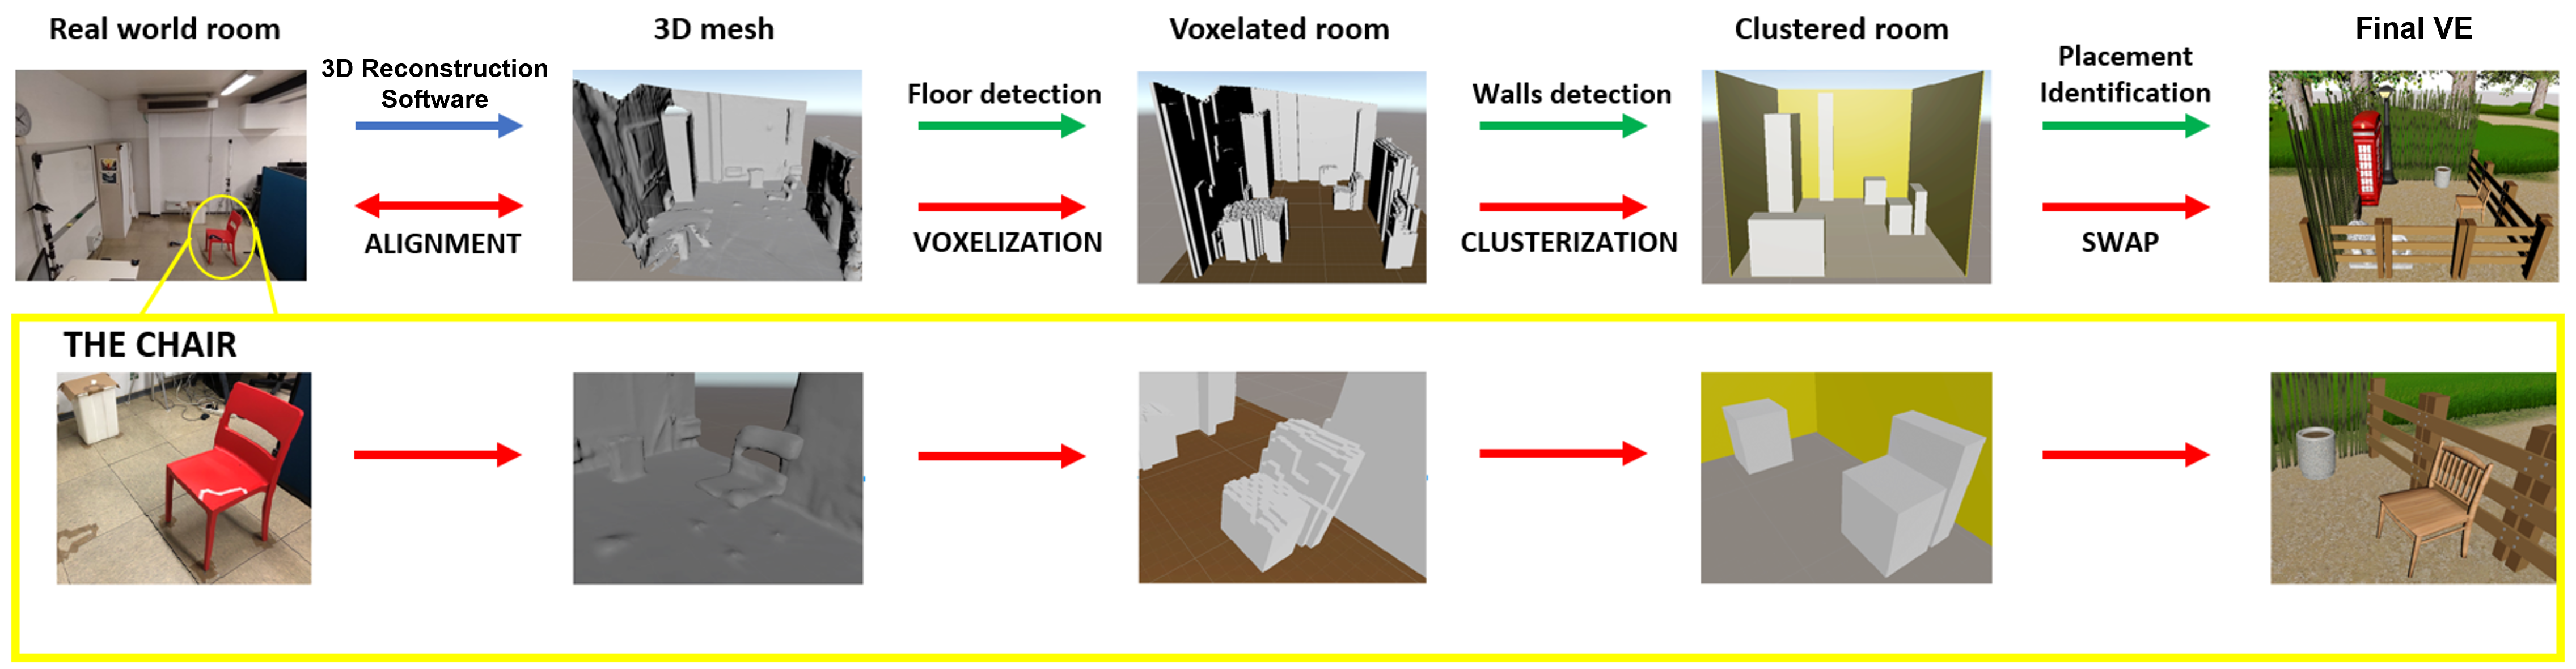
\includegraphics[width=0.9\columnwidth]{figures/intro/3d.png}
		
		\small Safety through spatial coherence 
		
		\column{0.33\textwidth}
		\centering
		\textbf{\textcolor{gbAqua}{Contribution 2}}
		
		\textit{Visualization Modalities}
		
		\includegraphics[width=0.9\columnwidth]{figures/intro/vm.png}
		
		\small Task effectiveness in non-immersive XR 
		
		\column{0.33\textwidth}
		\centering
		\textbf{\textcolor{gbAqua}{Contribution 3}}
		
		\textit{ActivePaws System}
		
		\includegraphics[width=0.9\columnwidth]{figures/intro/ap.png}
		
		\small Engagement in pediatric rehab 
	\end{columns}
\end{frame}

%% ══════════════════════════════════════════════════════════════════════════════
%% PART 2: THEORETICAL FOUNDATIONS (6 SLIDES)
%% ══════════════════════════════════════════════════════════════════════════════

\begin{frame}{Key Concepts: Definitions}
	\textbf{\textcolor{gbAqua}{Immersion}}: objective, technology-driven property
	\begin{itemize}
		\item Five key qualities: Extensive, Surrounding, Inclusive, Vivid, Matching
		\item Achieved through high-res visuals, spatialized audio, haptic feedback
	\end{itemize}

	\vspace{0.18cm}
	\textbf{\textcolor{gbAqua}{Presence}}: subjective psychological state
	\begin{itemize}
		\item Felt sense of ``being there'' in a virtual environment
		\item Three subscales: Spatial Presence, Involvement, Experienced Realism
	\end{itemize}

	\vspace{0.18cm}
	\textbf{\textcolor{gbAqua}{Usability}}: ease of use and effectiveness of a system
	\begin{itemize}
		\item Perceived simplicity, learnability, efficiency, memorability, error frequency, and user satisfaction 
	\end{itemize}

	\vspace{0.18cm}
	\textbf{\textcolor{gbAqua}{Cognitive Load}}: subjective mental workload
	\begin{itemize}
		\item Mental, physical, and temporal demand experienced during a task
	\end{itemize}

	\vspace{0.18cm}
	\textbf{\textcolor{gbAqua}{Engagement}}: depth of user investment
	\begin{itemize}
		\item Cognitive, temporal, affective, and behavioral involvement with a system
	\end{itemize}

	\citefooter{Steuer, 1992; Slater, 1997}
\end{frame}

\begin{frame}{Key Concepts: Questionnaires Used}
	\textbf{\textcolor{gbAqua}{Presence}} $\rightarrow$ IPQ (IGroup Presence Questionnaire)
	\begin{itemize}
		\item 14 items, 7-point Likert-type scale: three subscales + general item
	\end{itemize}

	\vspace{0.2cm}
	\textbf{\textcolor{gbAqua}{Usability}} $\rightarrow$ SUS (System Usability Scale)
	\begin{itemize}
		\item 10 items, 5-point Likert-type scale: score rescaled 1--100 (68 = average)
		\item SUS for Kids adaptation used for pediatric population
	\end{itemize}

	\vspace{0.2cm}
	\textbf{\textcolor{gbAqua}{Cognitive Load}} $\rightarrow$ RTLX (Raw NASA-TLX)
	\begin{itemize}
		\item 6 items rated on a 100-point scale
	\end{itemize}

	\vspace{0.2cm}
	\textbf{\textcolor{gbAqua}{Engagement}} $\rightarrow$ UES-SF (User Engagement Scale - Short Form)
	\begin{itemize}
		\item 12 items across 4 dimensions: Focused Attention, Perceived Usability, Aesthetic Appeal, Reward
	\end{itemize}

	\citefooter{Schubert et al., 1999; Brooke, 1996; Putnam et al., 2020; Hart \& Staveland, 1988; O'Brien et al., 2018}
\end{frame}



%% ══════════════════════════════════════════════════════════════════════════════
%% PART 3: STUDY 1 - 3D RECONSTRUCTION (9 SLIDES)
%% ══════════════════════════════════════════════════════════════════════════════
%% --- SEPARATORE ---
\begin{frame}[plain]
	\vfill
	\begin{center}
		{\large \textcolor{gbAqua}{\textbf{Contribution 1}}}
		
		\vspace{0.4cm}
		
		{\LARGE \textbf{Safety: Spatial Coherence Between Real and Virtual Environments}}
		%% {\LARGE \textbf{Safety in XR Environments through 3D Reconstruction}}
		
		\vspace{0.4cm}
	\end{center}
	\vfill
\end{frame}


\begin{frame}{Passive Haptics}
	\textbf{\textcolor{gbAqua}{The Challenge}}: Standard VR lacks tactile and haptic feedback
	
	\begin{itemize}
		\item Users cannot naturally sit on chairs, feel physical resistance
		\item Limits realism 
	\end{itemize}
	
	\vspace{0.3cm}
	
	\textbf{\textcolor{gbAqua}{The Solution}}: Co-register real objects with virtual counterparts
	
	\begin{itemize}
		\item No additional wearable hardware
		\item Low-cost, scalable approach
		\item Provides realistic tactile and proprioceptive cues
	\end{itemize}
	
	\vspace{0.3cm}
	
	\textbf{\textcolor{gbAqua}{Benefits}} (Evidence-Based)
	
	\begin{itemize}
		\item Enhanced presence and immersion
		\item More natural, ecologically valid movements
		\item Improved task performance (accuracy, speed)
	\end{itemize}
	
	\citefooter{Lindeman et al., 1999; McAnally \& Wallis, 2022}
\end{frame}\begin{frame}{Safety in XR: Obstacle Avoidance Challenge}
	\begin{columns}[T]
		\column{0.62\textwidth}
		\textbf{\textcolor{gbAqua}{The Problem}}


		Users are unaware of real obstacles; risk of collision, falls, injury
		
		\textbf{\textcolor{gbAqua}{Current Solutions}}
		
		\small
		\begin{itemize}
			\setlength\itemsep{0em}
			\vspace{-0.3cm}
			\item Guardian (Meta), Chaperone (HTC Vive): Static perimeter detection
			\item Scene Understanding (Meta Quest 3): Real-time 3D reconstruction
			\item Limitation: Fixed semantic categories
		\end{itemize}
		
		\column{0.35\textwidth}
		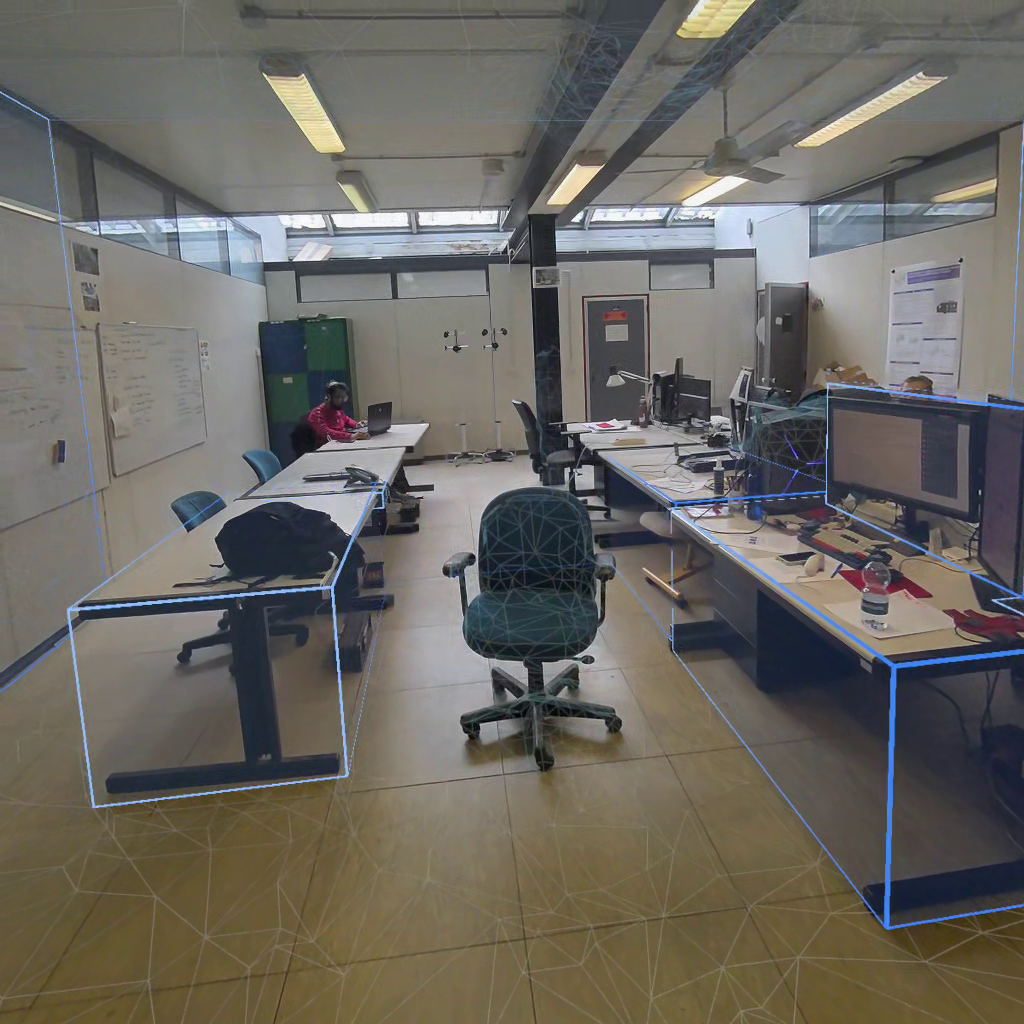
\includegraphics[width=\columnwidth]{figures/SOTA/1.png}
	\end{columns}
	
	\vfill
	\citefooter{Meta Developer Documentation}
\end{frame}

%% ══════════════════════════════════════════════════════════════════════════════
%% PART 3: CONTRIBUTION 1 — 3D RECONSTRUCTION (cappellino introduttivo)
%% ══════════════════════════════════════════════════════════════════════════════


%% --- SLIDE 1: MOTIVAZIONE ---
\begin{frame}{An Unexplored XR Application}
	
	One of the most compelling uses of XR lies in combining physical and virtual environments: for example, for simulation and training.
	
	\vspace{0.3cm}
	
	\textbf{\textcolor{gbAqua}{An example scenario}}
	
	A generic office is transformed into a virtual industrial plant for safety training. 
	Physical furniture becomes the scaffolding for the virtual layer: users sit on real chairs, lean on real tables, while perceiving them as part of the virtual environment. 
	This unlocks \textbf{passive haptics}: realistic tactile feedback with no additional hardware.
	
	\vspace{0.3cm}
	
	\textbf{\textcolor{gbAqua}{What such a system would need}}
	
	A spatial representation of the real environment: approximate object location, size, and layout.
	
	\vspace{0.2cm}
	
	\alert{Geometric perfection is not required}: coarse spatial alignment between physical and virtual layers is sufficient.
\end{frame}

\begin{frame}{Spatial Coherence: Passive Haptics + 3D Reconstruction Pipeline}

	\begin{center}
		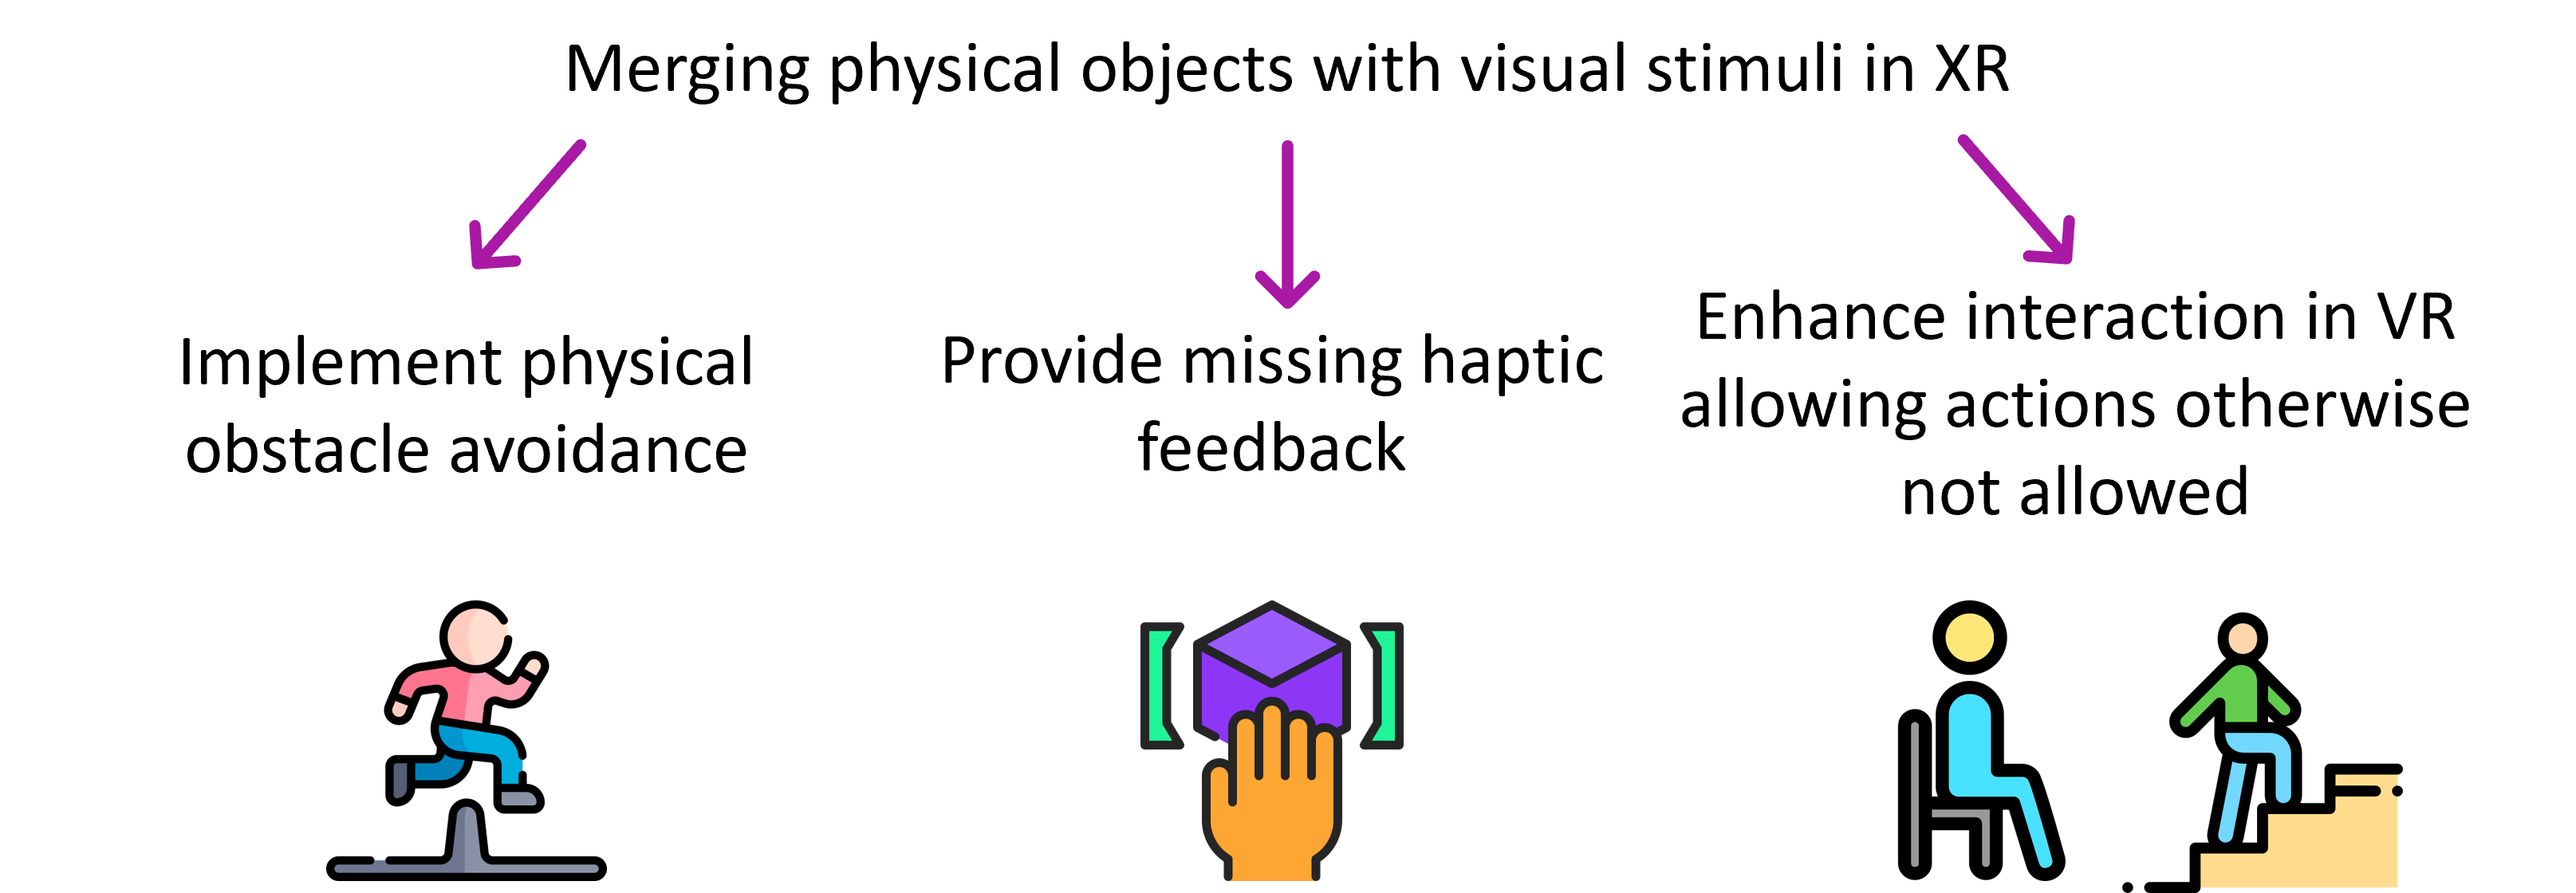
\includegraphics[width=\textwidth, height=0.41\textheight, keepaspectratio]{figures/obs.png}
	\end{center}
	\textbf{\textcolor{gbAqua}{Dual Function Approach}}	
	\begin{itemize}
		\item System that is simultaneously aware of physical layout AND maps virtual objects onto real counterparts
		\item Provides both safety guarantees and natural haptic feedback within same pipeline
		\item Reframes physical objects: from obstacles to interaction assets
	\end{itemize}
		
	\citefooter{Valentini et al., 2020; Wheeler et al., 2024}
\end{frame}


%% ══════════════════════════════════════════════════════════════════════════════
%% STUDY 2: FUNCTIONAL EVALUATION IN REAL ROOMS
%% ══════════════════════════════════════════════════════════════════════════════

\begin{frame}{Study 1}
    \textbf{\textcolor{gbAqua}{Evaluation of 3D Reconstruction Techniques for the Blending of Real and Virtual Environments}}
    
    \vspace{0.5cm}
    
    \small\textit{Based on:}
    
    \vspace{0.2cm}
    
    {\footnotesize M. Pizzo, et al., ``Evaluation of 3D Reconstruction Techniques for the Blending of Real and Virtual Environments,'' IEEE VRW, 2024}
\end{frame}


%% --- SLIDE 1A: GOAL ---
\begin{frame}{Study 1: Goal}
	\textbf{\textcolor{gbAqua}{From Benchmark to Real World Application}}

	Building on Study 1, this study moves to a real world scenario: creating XR environments where virtual objects are spatially registered onto real ones for \textbf{obstacle avoidance} and \textbf{passive haptics}.

	\vspace{0.4cm}

	\textbf{\textcolor{gbAqua}{Research Question}}

	\vspace{0.15cm}

	Do off-the-shelf 3D reconstruction techniques produce meshes that
are functionally sufficient as input for an XR pipeline designed for obstacle
avoidance and passive haptic interaction in real indoor environments?
	\vspace{0.3cm}

	\alert{Required precision is not fixed}: coarse alignment suffices for safe navigation and passive haptic interaction, whereas fine grained manipulation would demand higher accuracy.

	\citefooter{Pizzo et al., ``Evaluation of 3D Reconstruction Techniques for XR,'' IEEE VRW, 2024}
\end{frame}



%% --- SLIDE 2: METHODOLOGY ---
\begin{frame}{Study 1: Methodology}
	\begin{columns}[t]
		\column{0.48\textwidth}
		\textbf{\textcolor{gbAqua}{Six Real Indoor Rooms}}: Aquarium (meeting room), Copy room, Kitchen, Our Lab, PhD students' room, Professors' common room
		\vspace{0.15cm}

		\textbf{\textcolor{gbAqua}{Objects per Room}}
		\begin{itemize}
			\item Daily use objects: bottle, sanitizer, coffee cup, notebook
			\item Trackers, controllers (for alignment)
			\item Chairs left in place (safety critical)
		\end{itemize}

		\column{0.48\textwidth}
		\textbf{\textcolor{gbAqua}{Reconstruction Techniques}}

		\textit{Active:}
		\begin{itemize}
			\item Microsoft Kinect v1 + Skanect
		\end{itemize}

		\textit{Passive (photogrammetry, default parameters):}
		\begin{itemize}
			\item Autodesk ReCap Photo
			\item 3DF Zephyr
			\item Metashape
			\item Meshroom
			\item Regard3D
		\end{itemize}
		
		\textbf{\textcolor{gbAqua}{Input Data}}
		\begin{itemize}
			\item 100 photos or video frames per room
			\item Redmi Note 8T smartphone
		\end{itemize}

		
	\end{columns}

	\citefooter{Pizzo et al., IEEE VRW, 2024}
\end{frame}

%% --- SLIDE 1B: XR PIPELINE ---
\begin{frame}{Study 1: The XR Pipeline}
	\begin{center}
		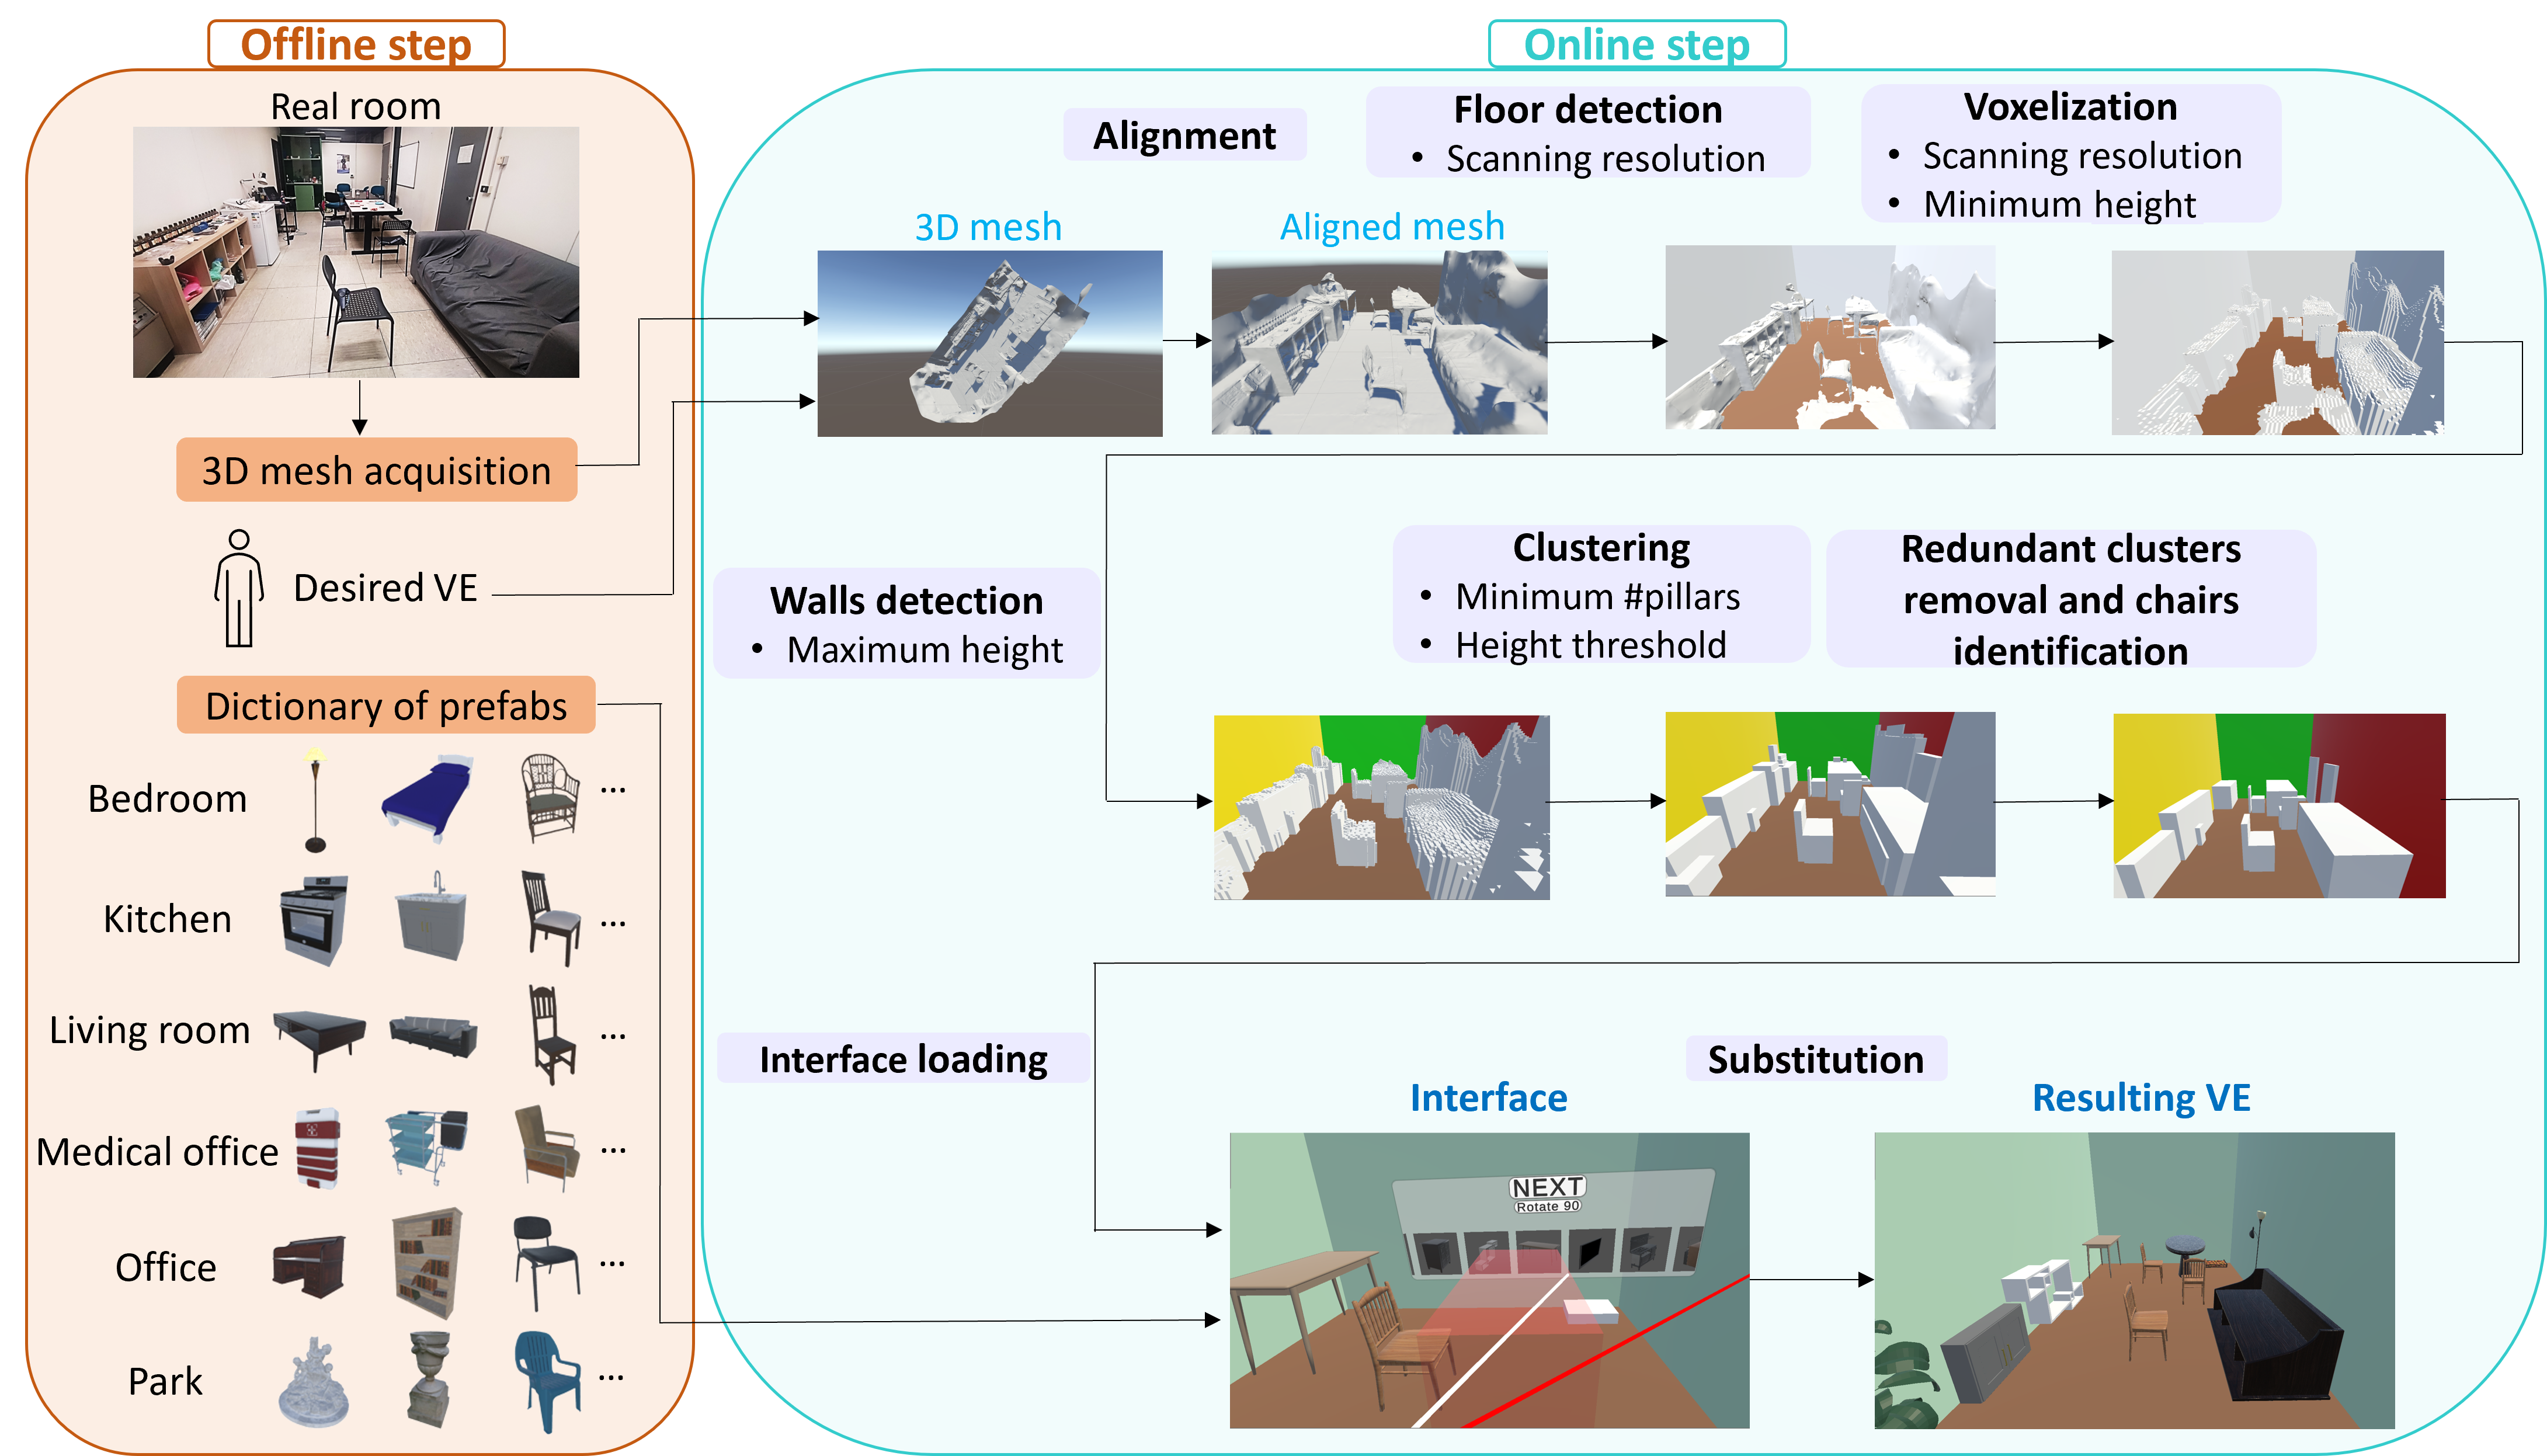
\includegraphics[width=\textwidth, height=0.78\textheight, keepaspectratio]{figures/PaperOrlando/pipeline3.png}
	\end{center}

	{\tiny XR system pipeline: 3D mesh → alignment → voxelization → clustering into bounding boxes → VR object substitution.}

	\citefooter{Pizzo et al., IEEE VRW, 2024}
\end{frame}


%% --- SLIDE 3: METRICS ---
\begin{frame}{Study 1: Evaluation Metrics}
	
	\begin{columns}[t]
		\column{0.48\textwidth}
		\textbf{Average Percentage Shift (APS)}

		Volume shift of reconstructed clusters vs.\ physically measured ground truth:
		\[
			APS_j = \frac{1}{N_j} \sum_{i=1}^{N_j} \left| \frac{V_{rec} - V_{gt}}{V_{gt}} \right| \times 100\%
		\]

		{\footnotesize where $i$ is the object index, $j$ is the room index, and $N_j$ is the number of objects in room $j$.}

		\vspace{0.2cm}

		\textbf{Chair Volume Shift} (separate)

		Safety critical: overestimation may lead user to sit where no physical surface exists.

		
		\column{0.48\textwidth}
		\textbf{Reconstruction Success Rate (RSR)}

		Fraction of object instances correctly reconstructed across the 6 rooms. For a specific object $A$ and software $s$:
		\[
			RSR_{A,s} = \frac{\sum_{j=1}^{6} NSR_{A,j}}{\sum_{j=1}^{6} IR_{A,j}} \times 100\%
		\]

		\vspace{0.2cm}

	\end{columns}

	\citefooter{Pizzo et al., IEEE VRW, 2024}
\end{frame}

%% --- SLIDE 4: ROOMS & RECONSTRUCTIONS ---
\begin{frame}{Study 1: Six Rooms and Their Reconstructions}
	\begin{center}
		\includegraphics[width=\textwidth, height=0.78\textheight, keepaspectratio]{figures/PaperOrlando/grid.png}
	\end{center}

	{\tiny Real rooms (col. 1), reconstructions with each technique, and XR pipeline clusters using ReCap Photo (last col.). Empty cells indicate reconstruction failure.}

	\citefooter{Pizzo et al., IEEE VRW, 2024}
\end{frame}



%% --- SLIDE 6: APS ---
\begin{frame}{Study 1 Results: Volume Accuracy}
	\begin{center}
		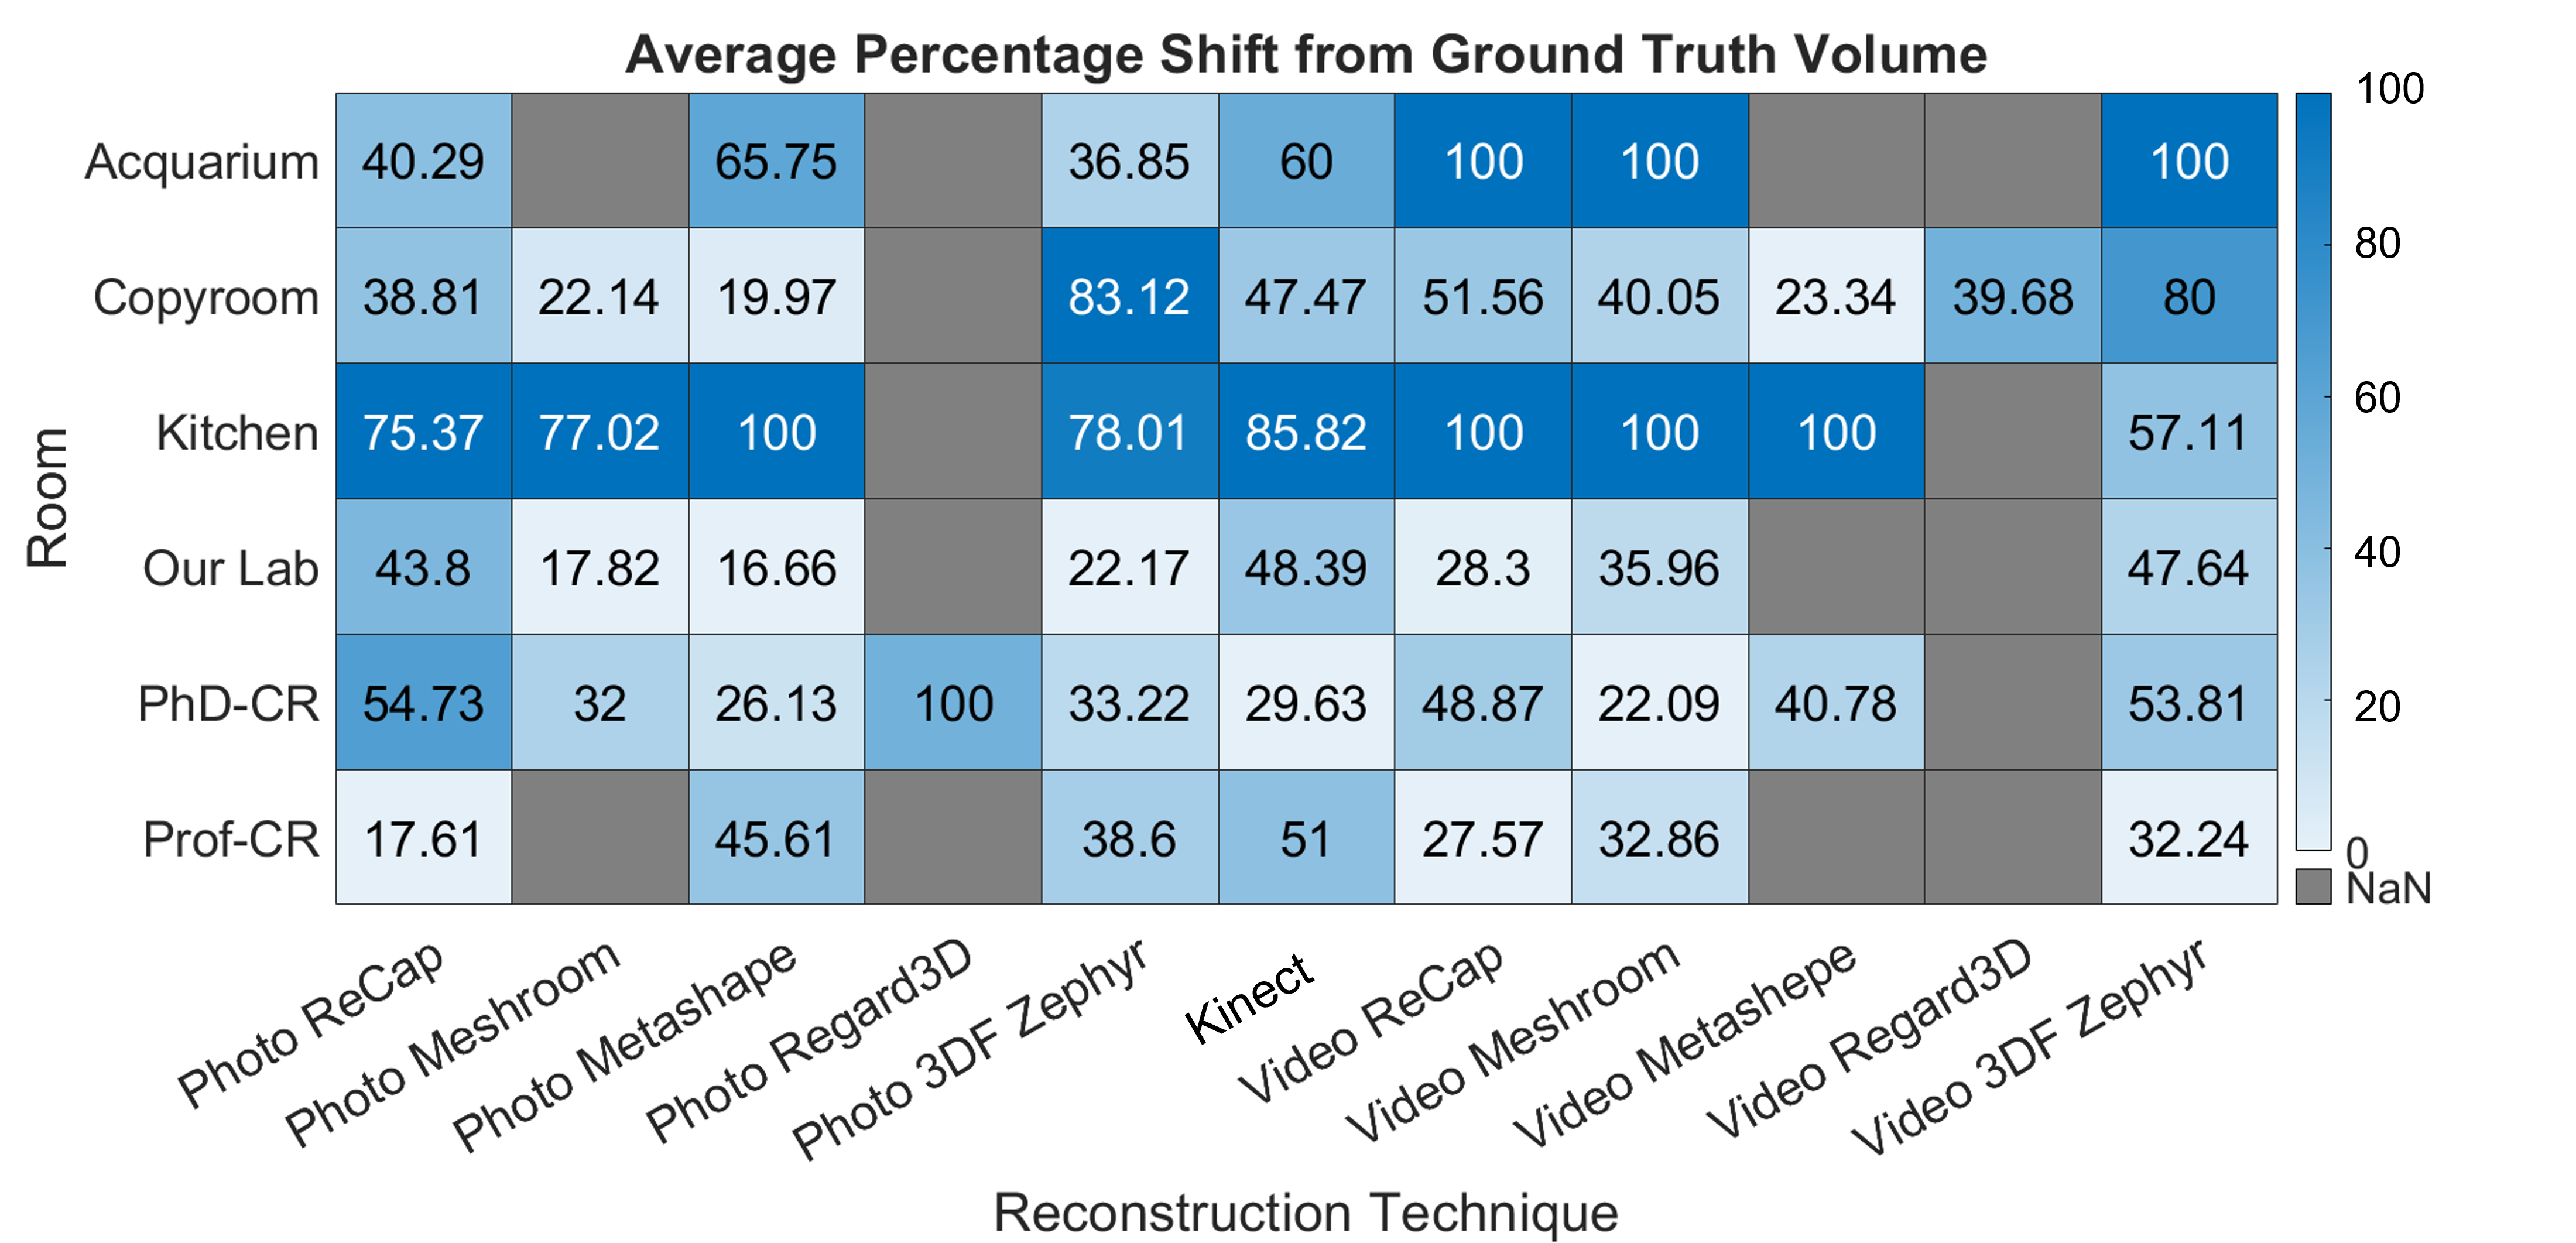
\includegraphics[width=\textwidth, height=0.72\textheight, keepaspectratio]{figures/PaperOrlando/heatmap.png}
	\end{center}

	{\tiny Some rooms (kitchen, aquarium) show high volume mismatch regardless of software, due to voxelization filling empty space. ReCap Photo with photos and Metashape achieve the lowest shift; video frames flatten performance across all software.}

	\citefooter{Pizzo et al., IEEE VRW, 2024}
\end{frame}

%% --- SLIDE: CHAIR VOLUME SHIFT ---
\begin{frame}{Study 1 Results: Chair Volume Accuracy}
	\begin{center}
		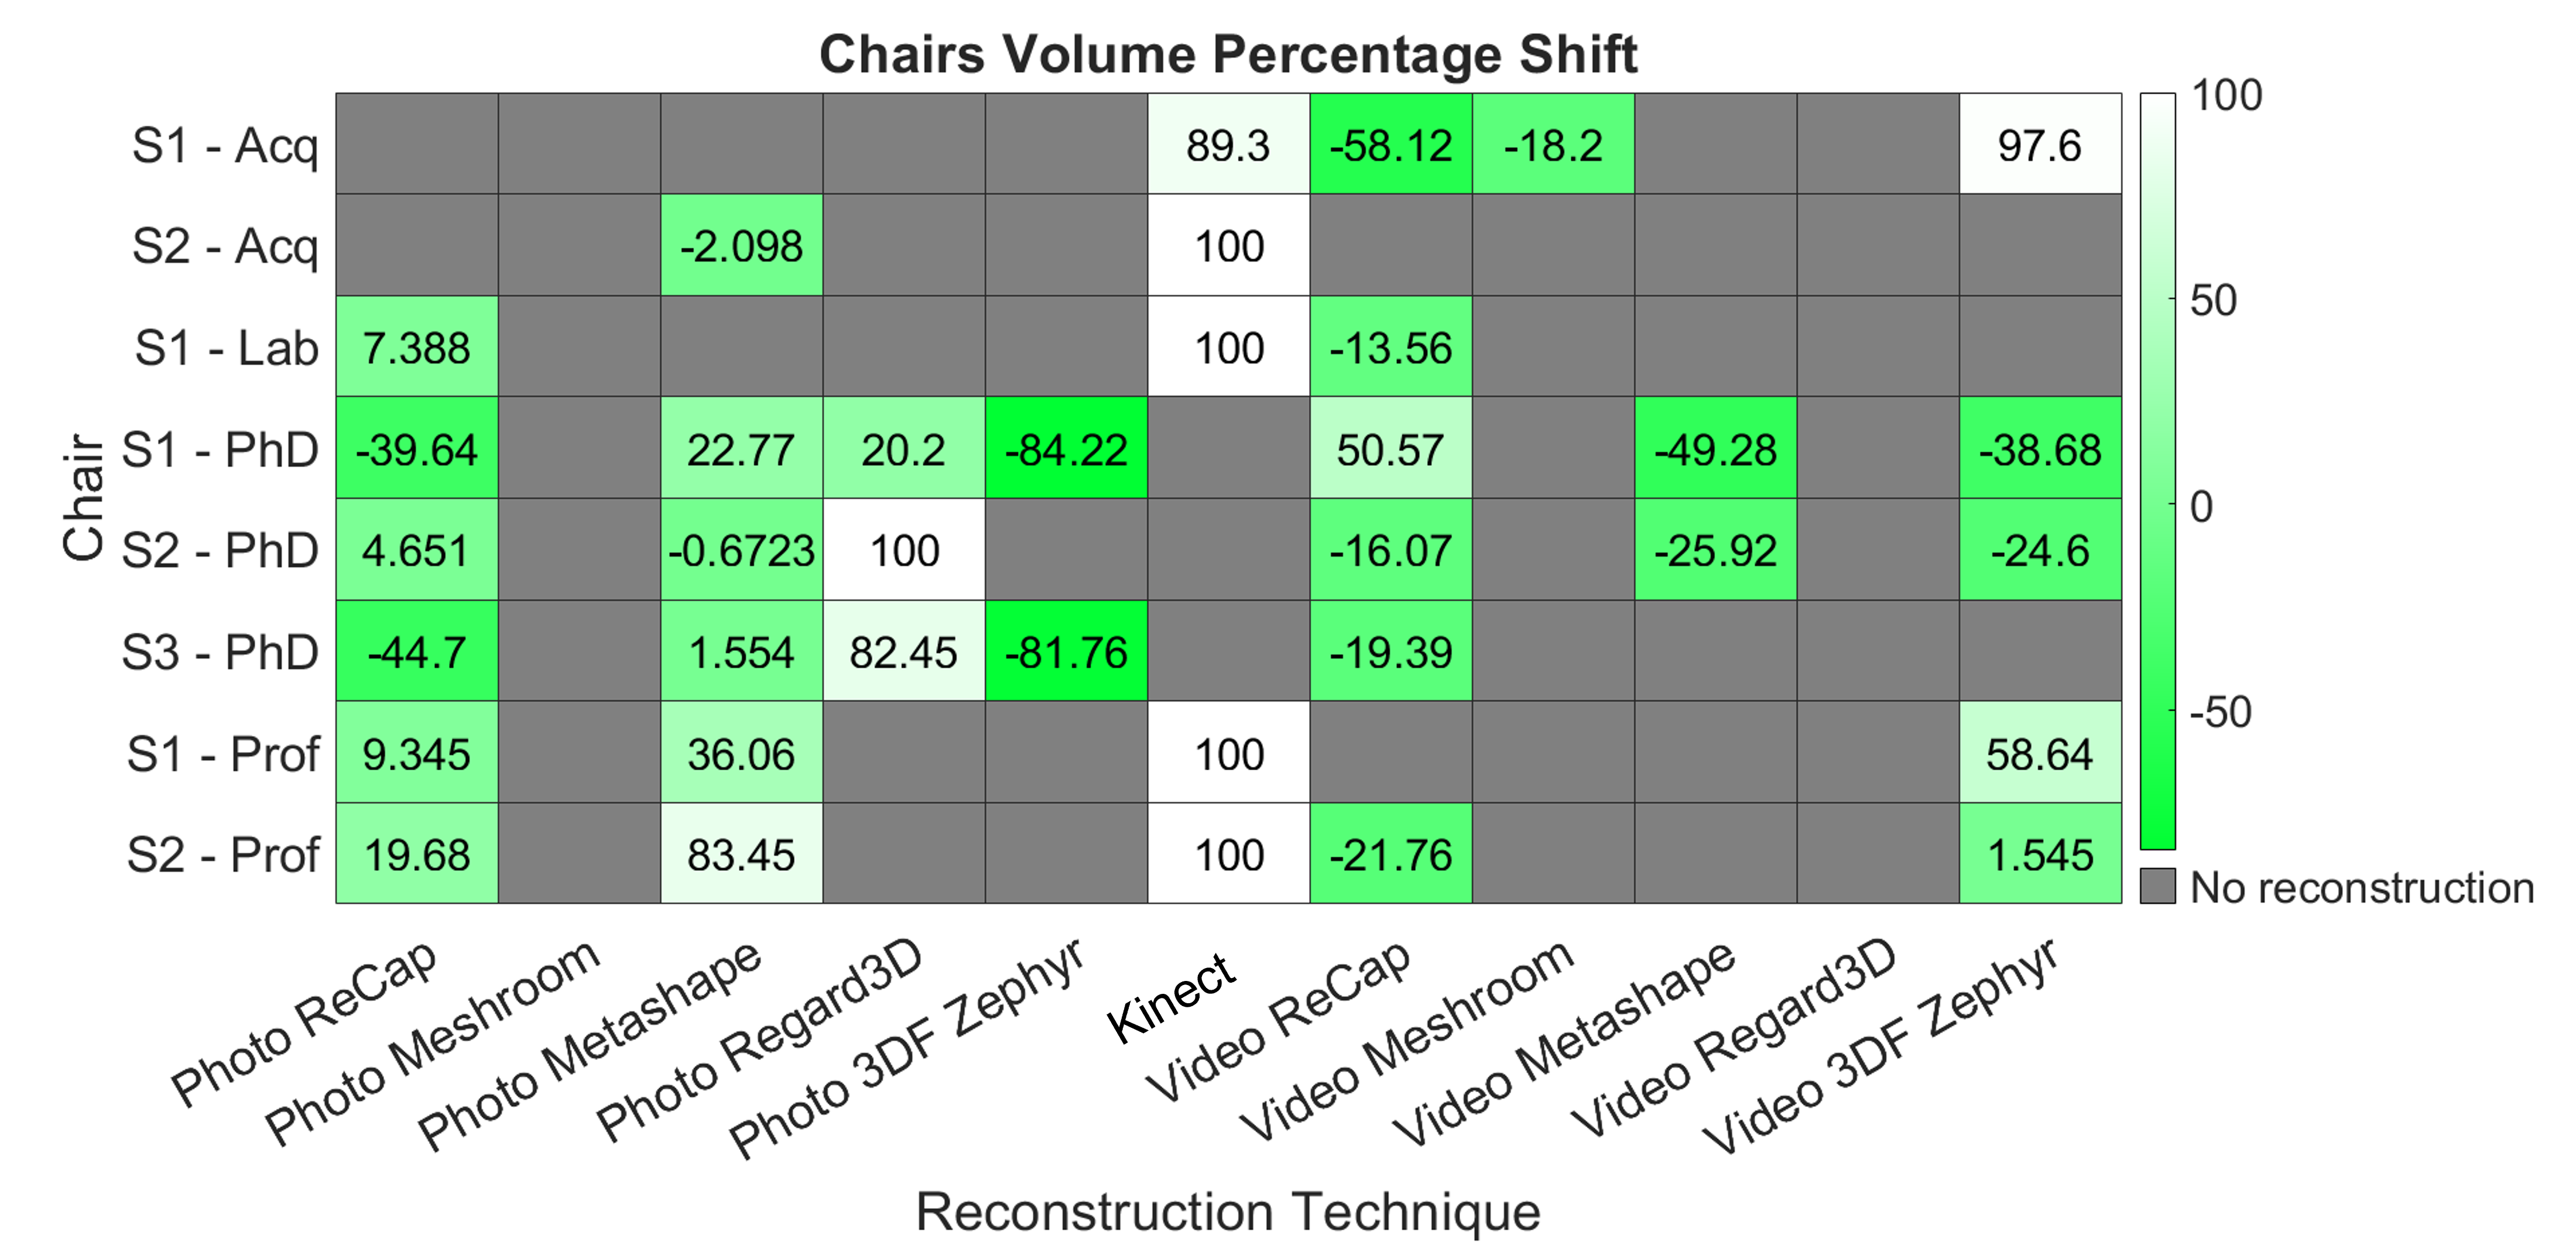
\includegraphics[width=\textwidth, height=0.72\textheight, keepaspectratio]{figures/PaperOrlando/heatmapChairs.png}
	\end{center}

	{\tiny Volume percentage shift of reconstructed chairs vs.\ ground truth. Positive values indicate overestimation (safety critical: user may attempt to sit where no surface exists). ReCap Photo is the most faithful; Skanect and 3DF Zephyr tend to overestimate significantly.}

	\citefooter{Pizzo et al., IEEE VRW, 2024}
\end{frame}

%% --- SLIDE 5: RSR ---
\begin{frame}{Study 1 Results: Reconstruction Success Rate}
	\begin{center}
		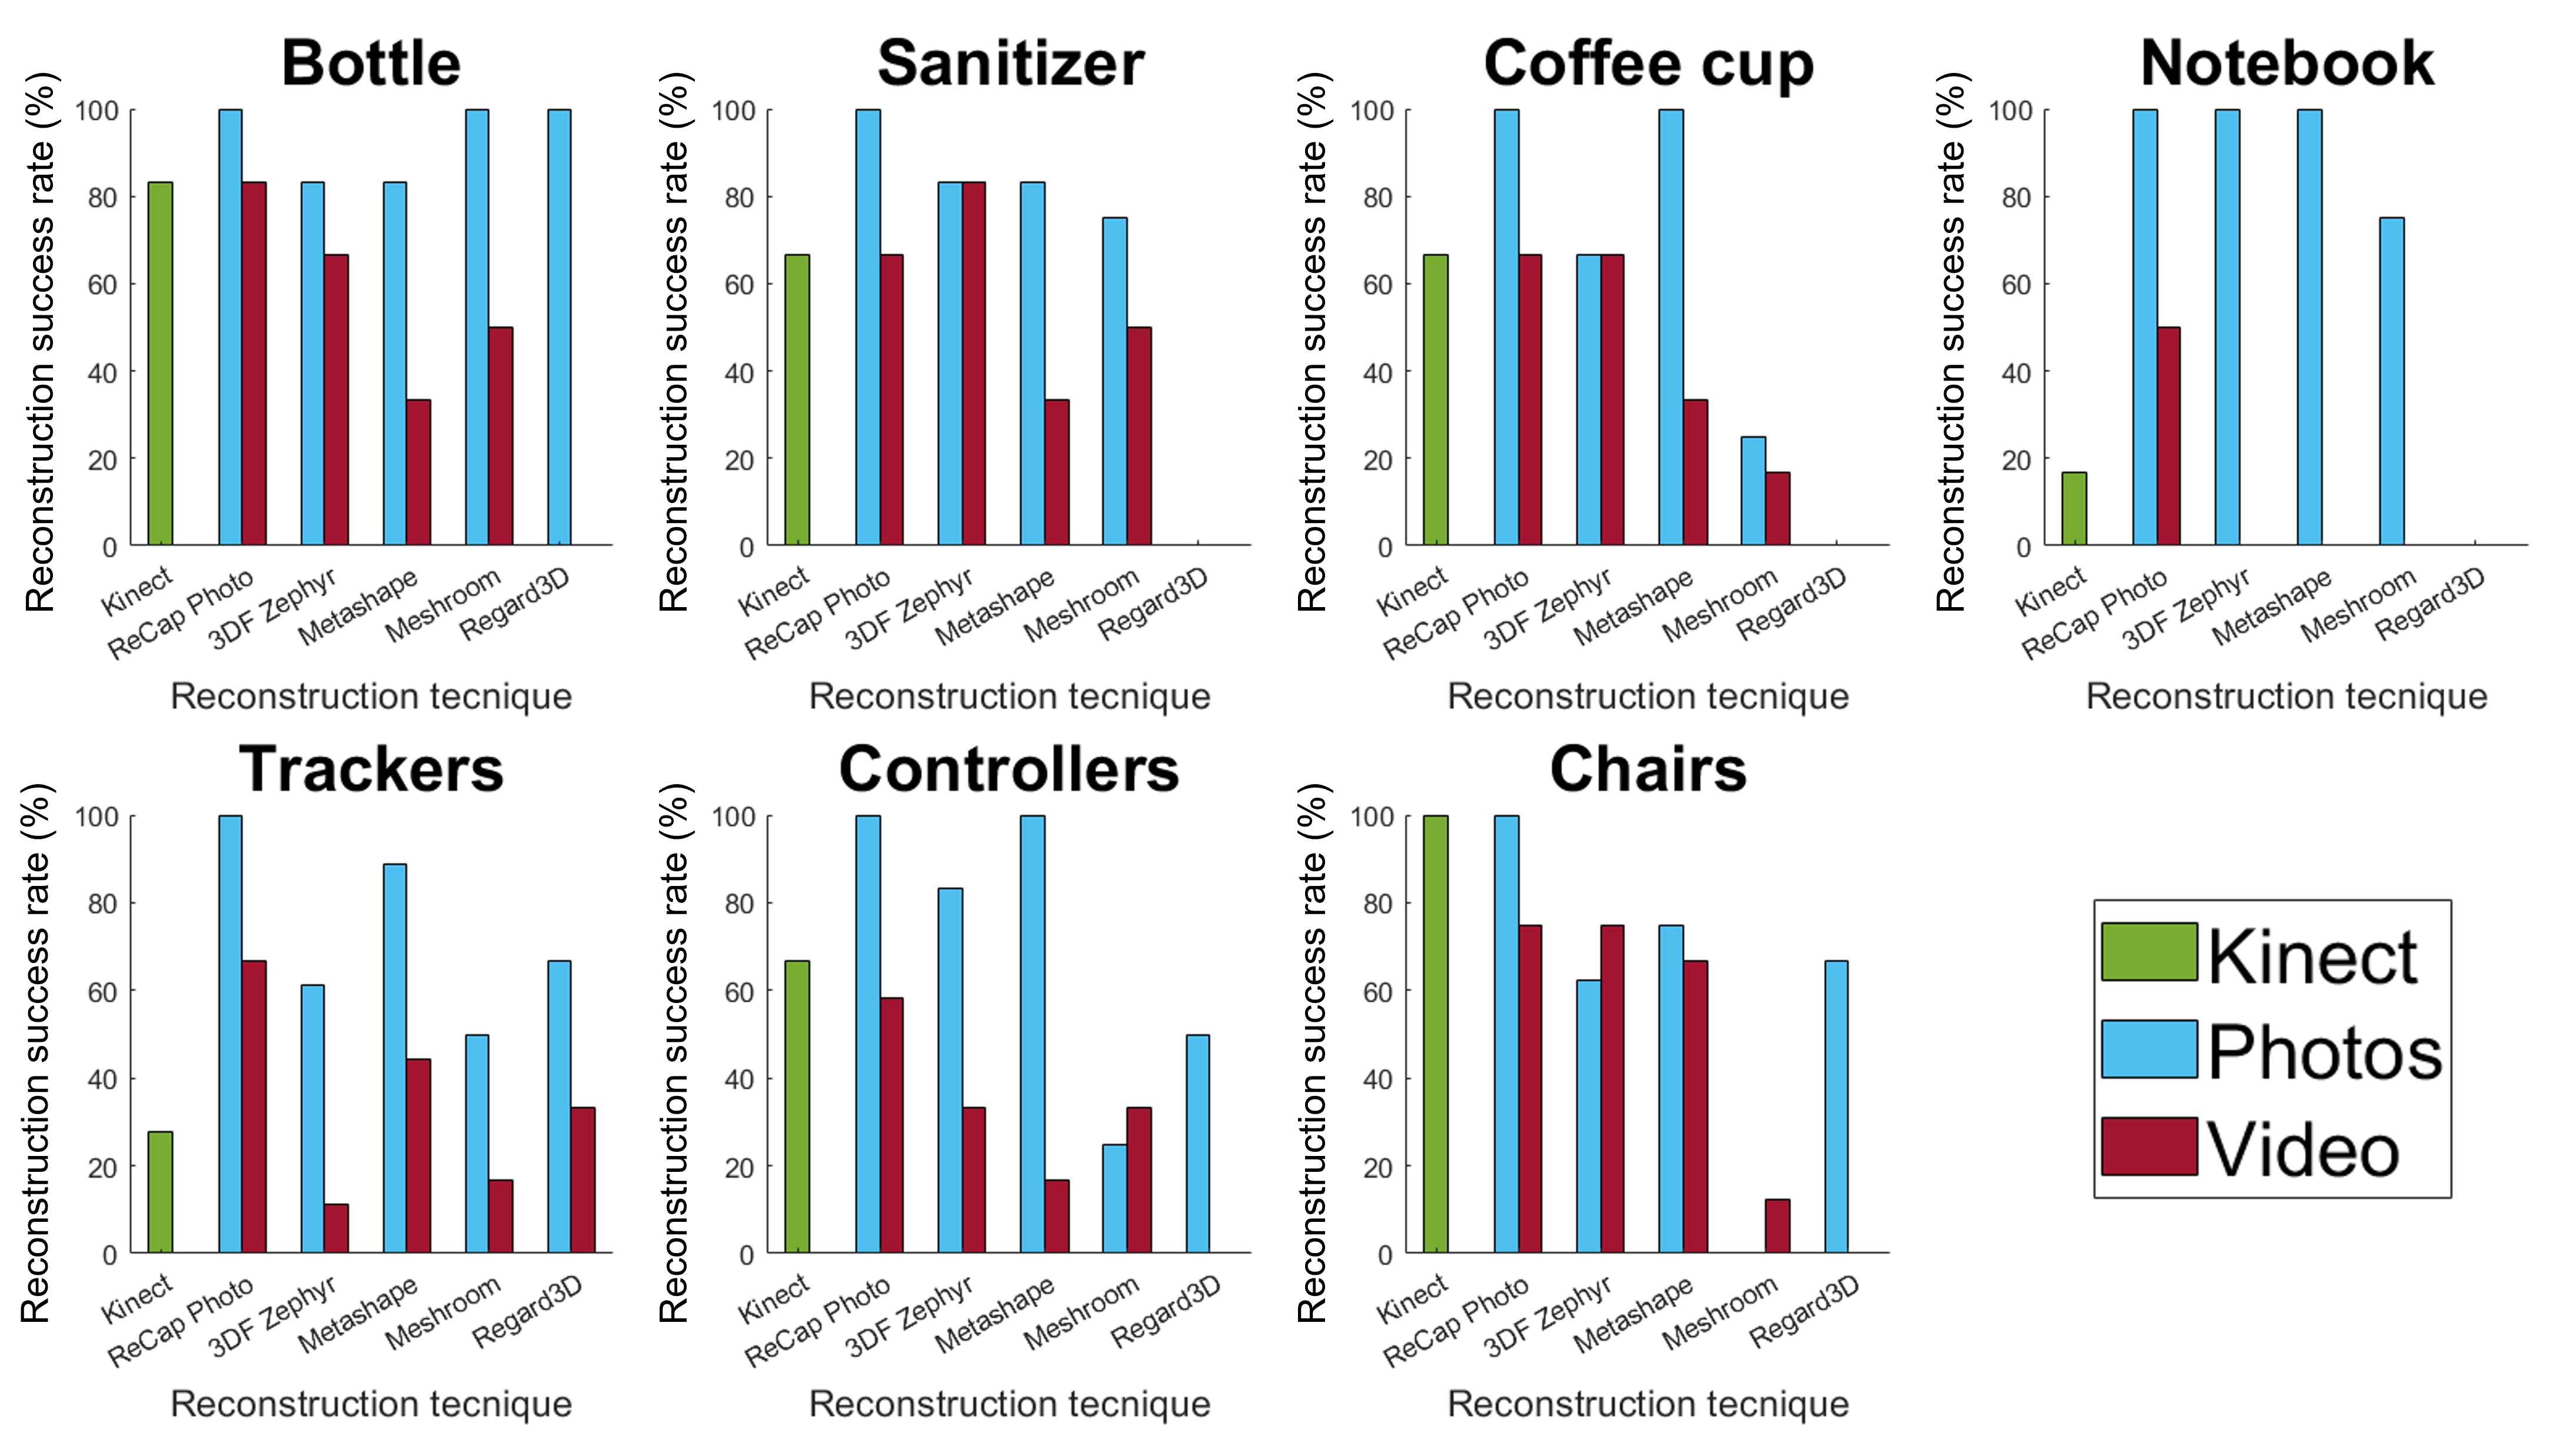
\includegraphics[width=\textwidth, height=0.72\textheight, keepaspectratio]{figures/PaperOrlando/tableResults.png}
	\end{center}

	{\tiny Protruding objects (bottle, sanitizer) easier to reconstruct than flat ones (notebook). Photos consistently outperform video frames. \alert{ReCap Photo and Kinect} are the only methods that always reconstruct chairs.}

	\citefooter{Pizzo et al., IEEE VRW, 2024}
\end{frame}

%% --- SLIDE 7: FINDINGS ---
\begin{frame}{Study 1: Findings}
	\begin{columns}[t]
		\column{0.48\textwidth}
		\textbf{\textcolor{gbAqua}{Per Technique Summary}}
		\begin{itemize}
			\item \textbf{ReCap Photo}: best RSR, faithful chair volumes, robust to image quality degradation
			\item \textbf{Kinect v1}: good RSR, fast acquisition ($<$3 min), struggles with small and flat objects
			\item \textbf{Metashape}: low APS with photos, but fails with video frames
			\item \textbf{3DF Zephyr, Meshroom, Regard3D}: higher failure rates or artifact generation
		\end{itemize}

		\column{0.48\textwidth}
		\textbf{\textcolor{gbAqua}{RQ Answer}}

		\vspace{0.1cm}

		Not all off-the-shelf techniques are sufficient, but several accessible ones are:

		\vspace{0.15cm}

		\alert{Autodesk ReCap Photo} (photos or video) and \alert{Kinect v1} produce reconstructions adequate for obstacle avoidance and passive haptics.

		\vspace{0.25cm}

	\end{columns}

	\citefooter{Pizzo et al., IEEE VRW, 2024}
\end{frame}



%% ══════════════════════════════════════════════════════════════════════════════
%% PART 4: STUDY 2 - VISUALIZATION MODALITIES (10 SLIDES)
%% ══════════════════════════════════════════════════════════════════════════════
%% ══════════════════════════════════════════════════════════════════════════════
%% PART 4: CONTRIBUTION 2 — VISUALIZATION MODALITIES
%% ══════════════════════════════════════════════════════════════════════════════

%% --- SEPARATORE ---
\begin{frame}[plain]
	\vfill
	\begin{center}
		{\large \textcolor{gbAqua}{\textbf{Contribution 2}}}
		
		\vspace{0.4cm}
		
		{\LARGE \textbf{Task Effectiveness: Comparison of Visualization Modalities for Motor Tasks}}
		
	\end{center}
	\vfill
\end{frame}

\begin{frame}{SOTA: Visualization Modalities in XR}
	\textbf{\textcolor{gbAqua}{Three Categories by Immersion Level}}
	
	\begin{itemize}
		\item \textbf{Non-immersive}: Screens that don't occlude FOV
		\item \textbf{Semi-immersive}: CAVE or multi-monitor (partial occlusion)
		\item \textbf{Immersive}: HMD-based (full FOV occlusion)
	\end{itemize}
	
	\vspace{0.3cm}
	
	\textbf{\textcolor{gbAqua}{Empirical Evidence}}
	
	Wenk et al. (2019-2023) systematically compared IVR, AR and non-immersive setups in reaching tasks with concurrent cognitive load (cognitive-motor dual task). They found:
	
	\begin{itemize}
		\item IVR improved motor performance and reduced cognitive load screen condition (nIVR)
		\item IVR rated more motivating and usable wrt AR and nIVR 
		\item IVR achieved higher embodiment than 2D screen 
		\item Gap: No study systematically compared different non-immersive projection types
	\end{itemize}
	
	\citefooter{Wenk et al., 2019, 2022, 2023; Bassano et al., 2022}
\end{frame}


\begin{frame}{Why Immersive VR Not Always Feasible in Clinical Settings}
	\textbf{\textcolor{gbAqua}{Clinical Reality}}
	
	HMD adoption barriers:
	
	\begin{itemize}
		\item \textbf{Patient factors}: Severe cognitive impairment, epilepsy, photosensitivity, rare conditions with unknown IVR applicability
		\item \textbf{Staff resistance}: Clinicians unwilling to adopt IVR technology
		\item \textbf{Visual contact}: Need to maintain caregiver supervision
		\item \textbf{Financial \& Logistical}: High cost, maintenance burden, need for specialized personnel, lack of HMDs in hospitals
	\end{itemize}
	
	\vspace{0.3cm}
	
	\textbf{\textcolor{gbAqua}{Result}}
	
	Most exergames and serious games rely on non-immersive setups, offering accessibility, affordability, and portability.
	\\We lose the benefits of IVR: high sense of presence and everything related to it.
	\\Little empirical guidance exists on which visualization modality is best.
	
	\citefooter{Ren et al., 2024; Bassano et al., 2022}
\end{frame}


%% --- PAPER REFERENCE ---
\begin{frame}{Study 3}
	\textbf{\textcolor{gbAqua}{Immersive versus Non-Immersive Virtual Reality Environments: Comparing Different Visualization Modalities in a Cognitive-Motor Dual-Task}}
	
	\vspace{0.5cm}
	
	\small\textit{Based on:}
	
	\vspace{0.2cm}
	
	{\footnotesize M. Pizzo, M. Martini, F. Solari, M. Chessa, ``Immersive versus Non-Immersive Virtual Reality Environments: Comparing Different Visualization Modalities in a Cognitive-Motor Dual-Task,'' VISIGRAPP, 2025}
\end{frame}

\begin{frame}{The Clinical Design Problem: Visualization Modalities}
	\textbf{\textcolor{gbAqua}{The Problem}}
	
	During development of non-immersive exergame for upper limb rehabilitation, using a reaching task, clinicians reported that perspective projection introduced visible distortion at screen periphery and they raised concerns about perspective breaking presence.\vspace{0.3cm}
	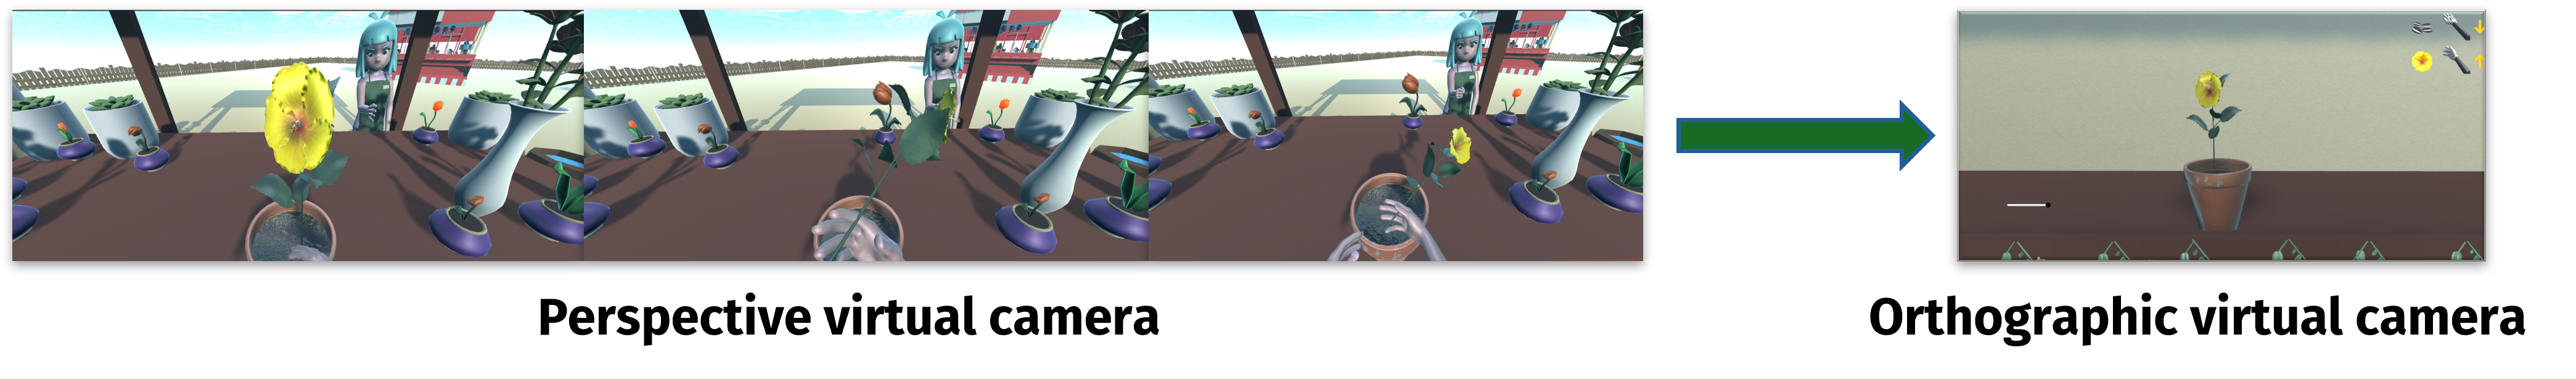
\includegraphics[width=1\columnwidth]{figures/VisualizationMod/problemb.png}
	\vspace{0.3cm}
	\textbf{\textcolor{gbAqua}{The Dilemma}}


	When IVR unavailable, which modality is best?

\end{frame}


\begin{frame}{Study 3: Comparing Four Visualization Modalities}
	\textbf{\textcolor{gbAqua}{Research Question}}
	
	When IVR is not feasible, which non-immersive VM best approximates its benefits in terms of sense of presence, usability, cognitive load, and task performance?
	
	\vspace{0.3cm}
	\includegraphics[width=0.7\columnwidth]{figures/intro/vm.png}

	
	\citefooter{Pizzo et al., ``Immersive versus Non-Immersive Virtual Reality in Cognitive-Motor Dual-Task,'' VISIGRAPP, 2025}
\end{frame}


\begin{frame}{Study 3: Three Hypotheses}
	\textbf{\textcolor{gbAqua}{Three Hypotheses we tested}}
	
	\begin{itemize}
		\item \textbf{H1}: IVR outperforms all non-immersive alternatives showing higher sense of presence, better usability, and lower cognitive load (control hypothesis)	
		\item \textbf{H2}: POV (tracked perspective) is the best approximation of VR in term of sense of presence, usability and cognitive load;
		\item \textbf{H3}: PERSP (fixed perspective) and ORTHO (orthographic) provide comparable sense of presence, usability, and cognitive load;
		\end{itemize}
\end{frame}

\begin{frame}{Study 3 Methodology: Four Visualization Modalities}
	\begin{columns}[T]		
		\column{0.3\textwidth}
		\vspace{2.5cm}
		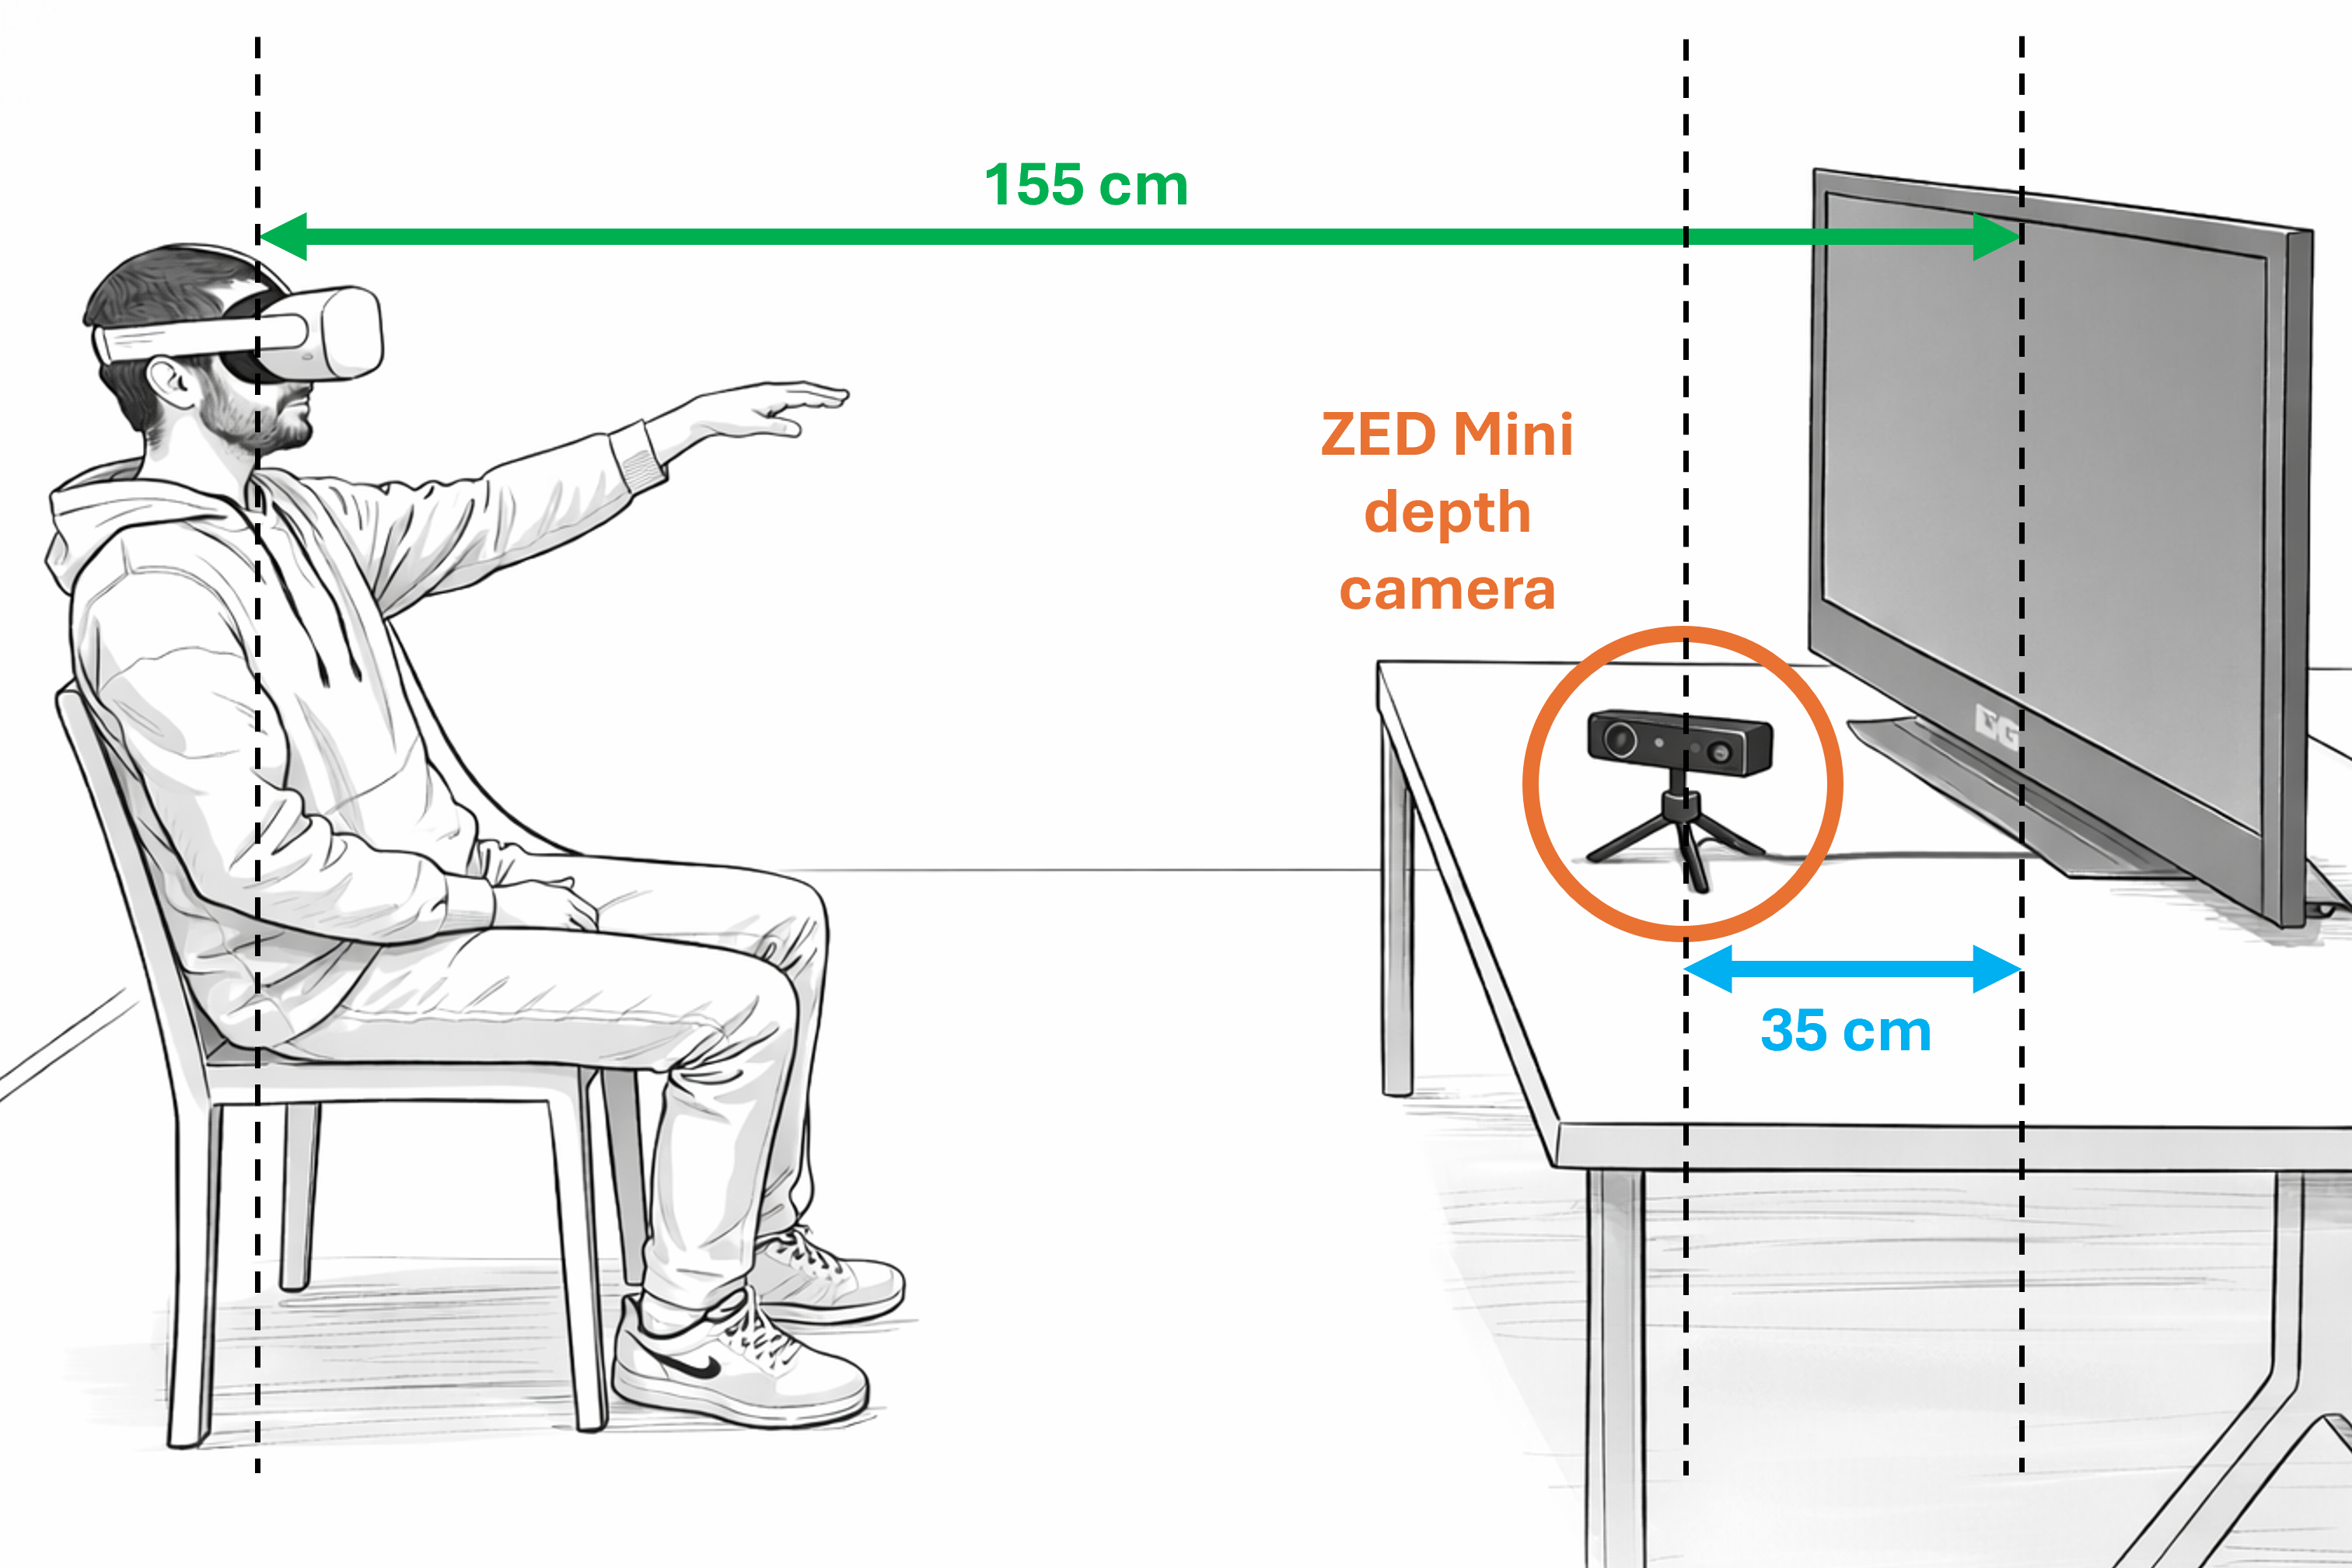
\includegraphics[width=\linewidth]{figures/VisualizationMod/enzo.png}
		
		
		\column{0.7\textwidth}
		All four conditions have full body avatar with only arms \& hands animated in sync.\\
		\textbf{\textcolor{gbAqua}{Shared non-immersive setup}}
		\begin{itemize}
			\item 47'' display screen
			\item ZED Mini stereo camera for 38-joint body tracking
		\end{itemize}
		
		\textbf{\textcolor{gbAqua}{Conditions}}
		\begin{itemize}
			\item \textbf{IVR}: Meta Quest 2 HMD, hand tracking
			\item \textbf{POV}: Perspective camera (75° FOV), pose updated with user's tracked 6DOF head position
			\item \textbf{PERSP}: Perspective camera (75° FOV, 7° downward tilt), fixed position
			\item \textbf{ORTHO}: Orthographic camera, viewport sized to keep all shelves in field of view, fixed position
		\end{itemize}
	\end{columns}
\end{frame}

\begin{frame}{Study 3 Methodology: Video Demonstration}
	\begin{center}
		\includegraphics[width=0.85\linewidth, height=0.55\textheight, keepaspectratio]{figures/VisualizationMod/VisMod.png}\\[0.3cm]
		\href{https://www.youtube.com/watch?v=k1AMaxmxgAM&t=3s}{%
			\textcolor{gbAqua}{\textbf{$\blacktriangleright$ Video}}%
		}
	\end{center}
	
	\citefooter{Pizzo et al., 2025}
\end{frame}



\begin{frame}{Study 3 Methodology: Task, Demographics and Measurements}
	\begin{columns}[T]
		\column{0.65\textwidth}
		\textbf{\textcolor{gbAqua}{Cognitive-Motor Dual Task (CMDT)}}
		\begin{itemize}
			\item Simultaneous motor + cognitive task: counting cats and touching only pink flowers
			\item 24 healthy subjects (8F, 16M), within-subject design
			\item 1 to 4 items displayed per trial, 28 trials
			\item IVR, then POV/PERSP/ORTHO in randomized order
			\item Tier list ranking collected at the end
		\end{itemize}
		\textbf{\textcolor{gbAqua}{Evaluation Metrics}}
		\begin{itemize}
			\item \textbf{Sense of Presence}: IPQ
			\item \textbf{Usability}: SUS
			\item \textbf{Cognitive Load}: Raw NASA-TLX
			\item \textbf{CMDT Performance}
		\end{itemize}
		
		\column{0.35\textwidth}
		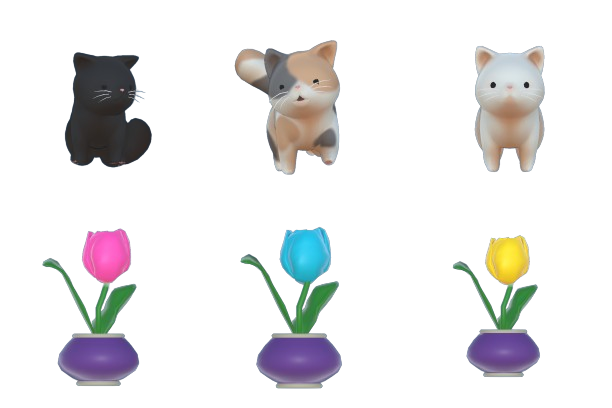
\includegraphics[width=\linewidth]{figures/VisualizationMod/OggettiSenzaSfondo.png}
		\vspace{0.2cm}
		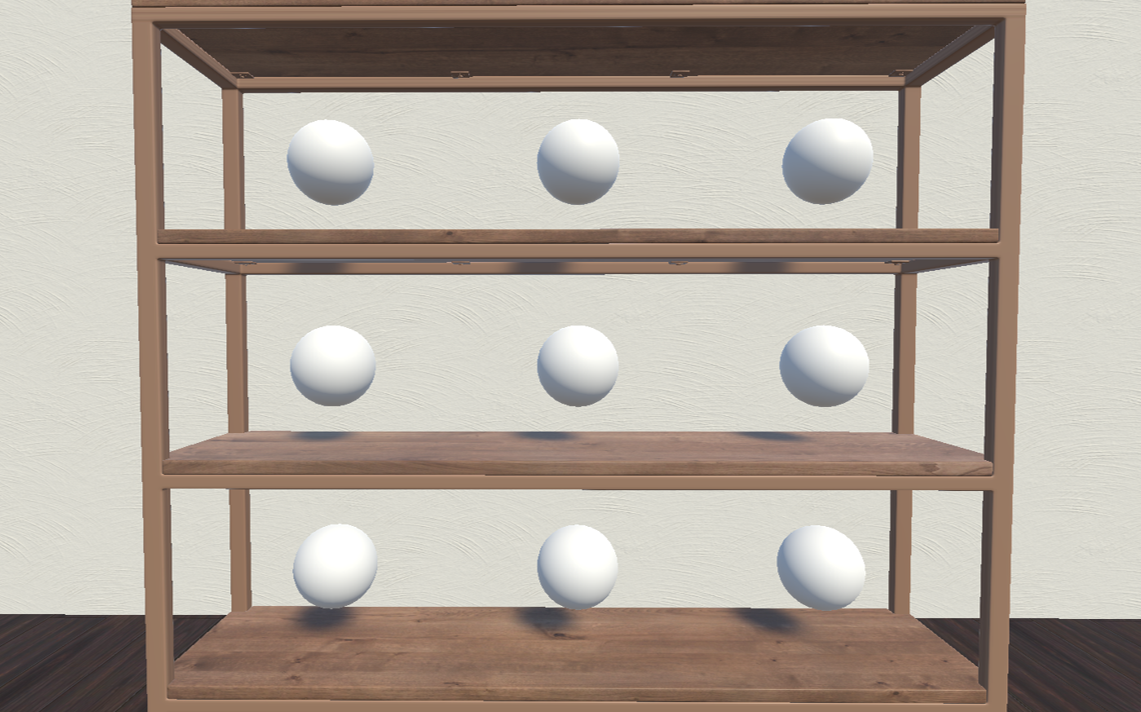
\includegraphics[width=\linewidth]{figures/VisualizationMod/shelving2.png}
	\end{columns}
	
	\citefooter{Schubert et al., 2001; Brooke, 1996; Hart \& Staveland, 1988}
\end{frame}

\begin{frame}{Study 3 Results: Sense of Presence}
	\begin{columns}[c]
		\column{0.3\textwidth}		
		\begin{itemize}
			\item Three IPQ subscales: spatial presence (SP), involvement (INV), realism (REAL). PRES refers to the general sense of ``being there''.
			\item VR significantly higher presence than all non-immersive 
			\item POV did NOT approximate VR well
		\end{itemize}
		
		\column{0.7\textwidth}
		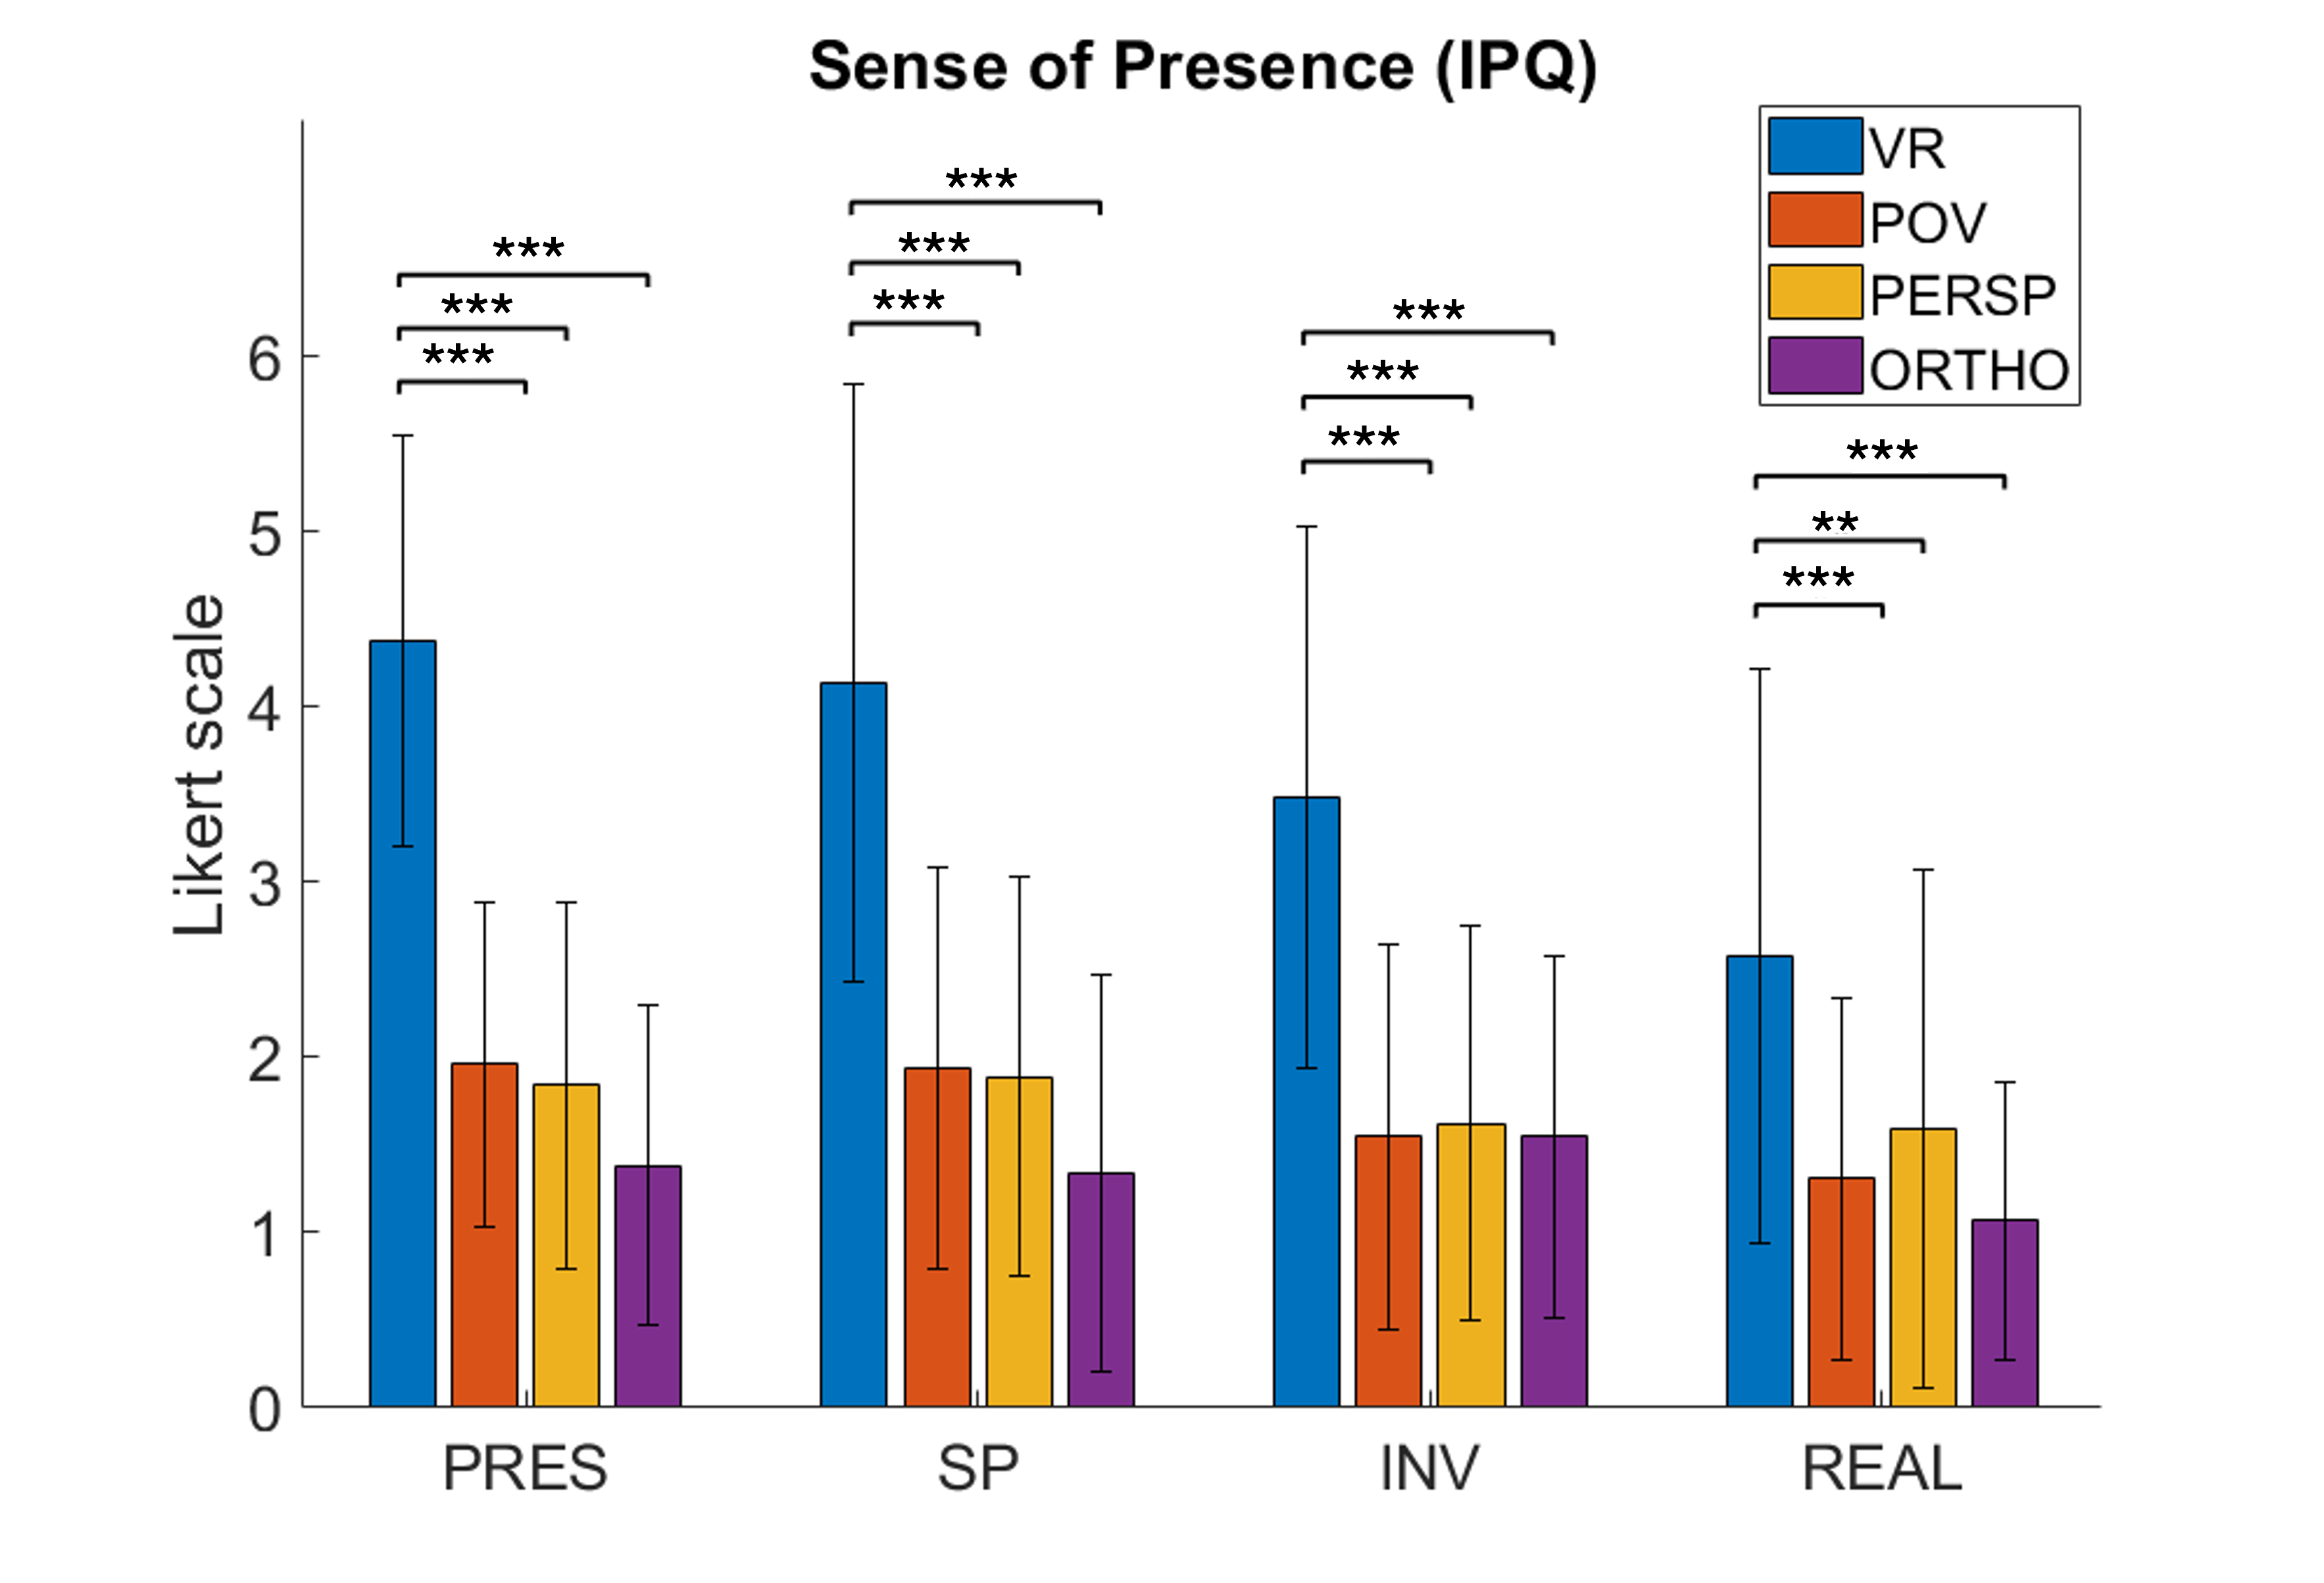
\includegraphics[width=\linewidth]{figures/VisualizationMod/Questionari/IPQ.png}
		
		{\tiny $^*p \leq 0.05$;\quad $^{**}p \leq 10^{-2}$;\quad $^{***}p \leq 10^{-3}$}
	\end{columns}
	
	\citefooter{Pizzo et al., 2025}
\end{frame}

\begin{frame}{Study 3 Results: Usability}
	\begin{columns}[c]
		\column{0.3\textwidth}
		\textbf{\textcolor{gbAqua}{From the literature}}
		\begin{itemize}
			\item AVG SUS score: 68
			\item SUS $<$ 51 indicates serious usability issues
			\item SUS $>$ 80.3 indicates excellent usability
		\end{itemize}
		
		\column{0.7\textwidth}
		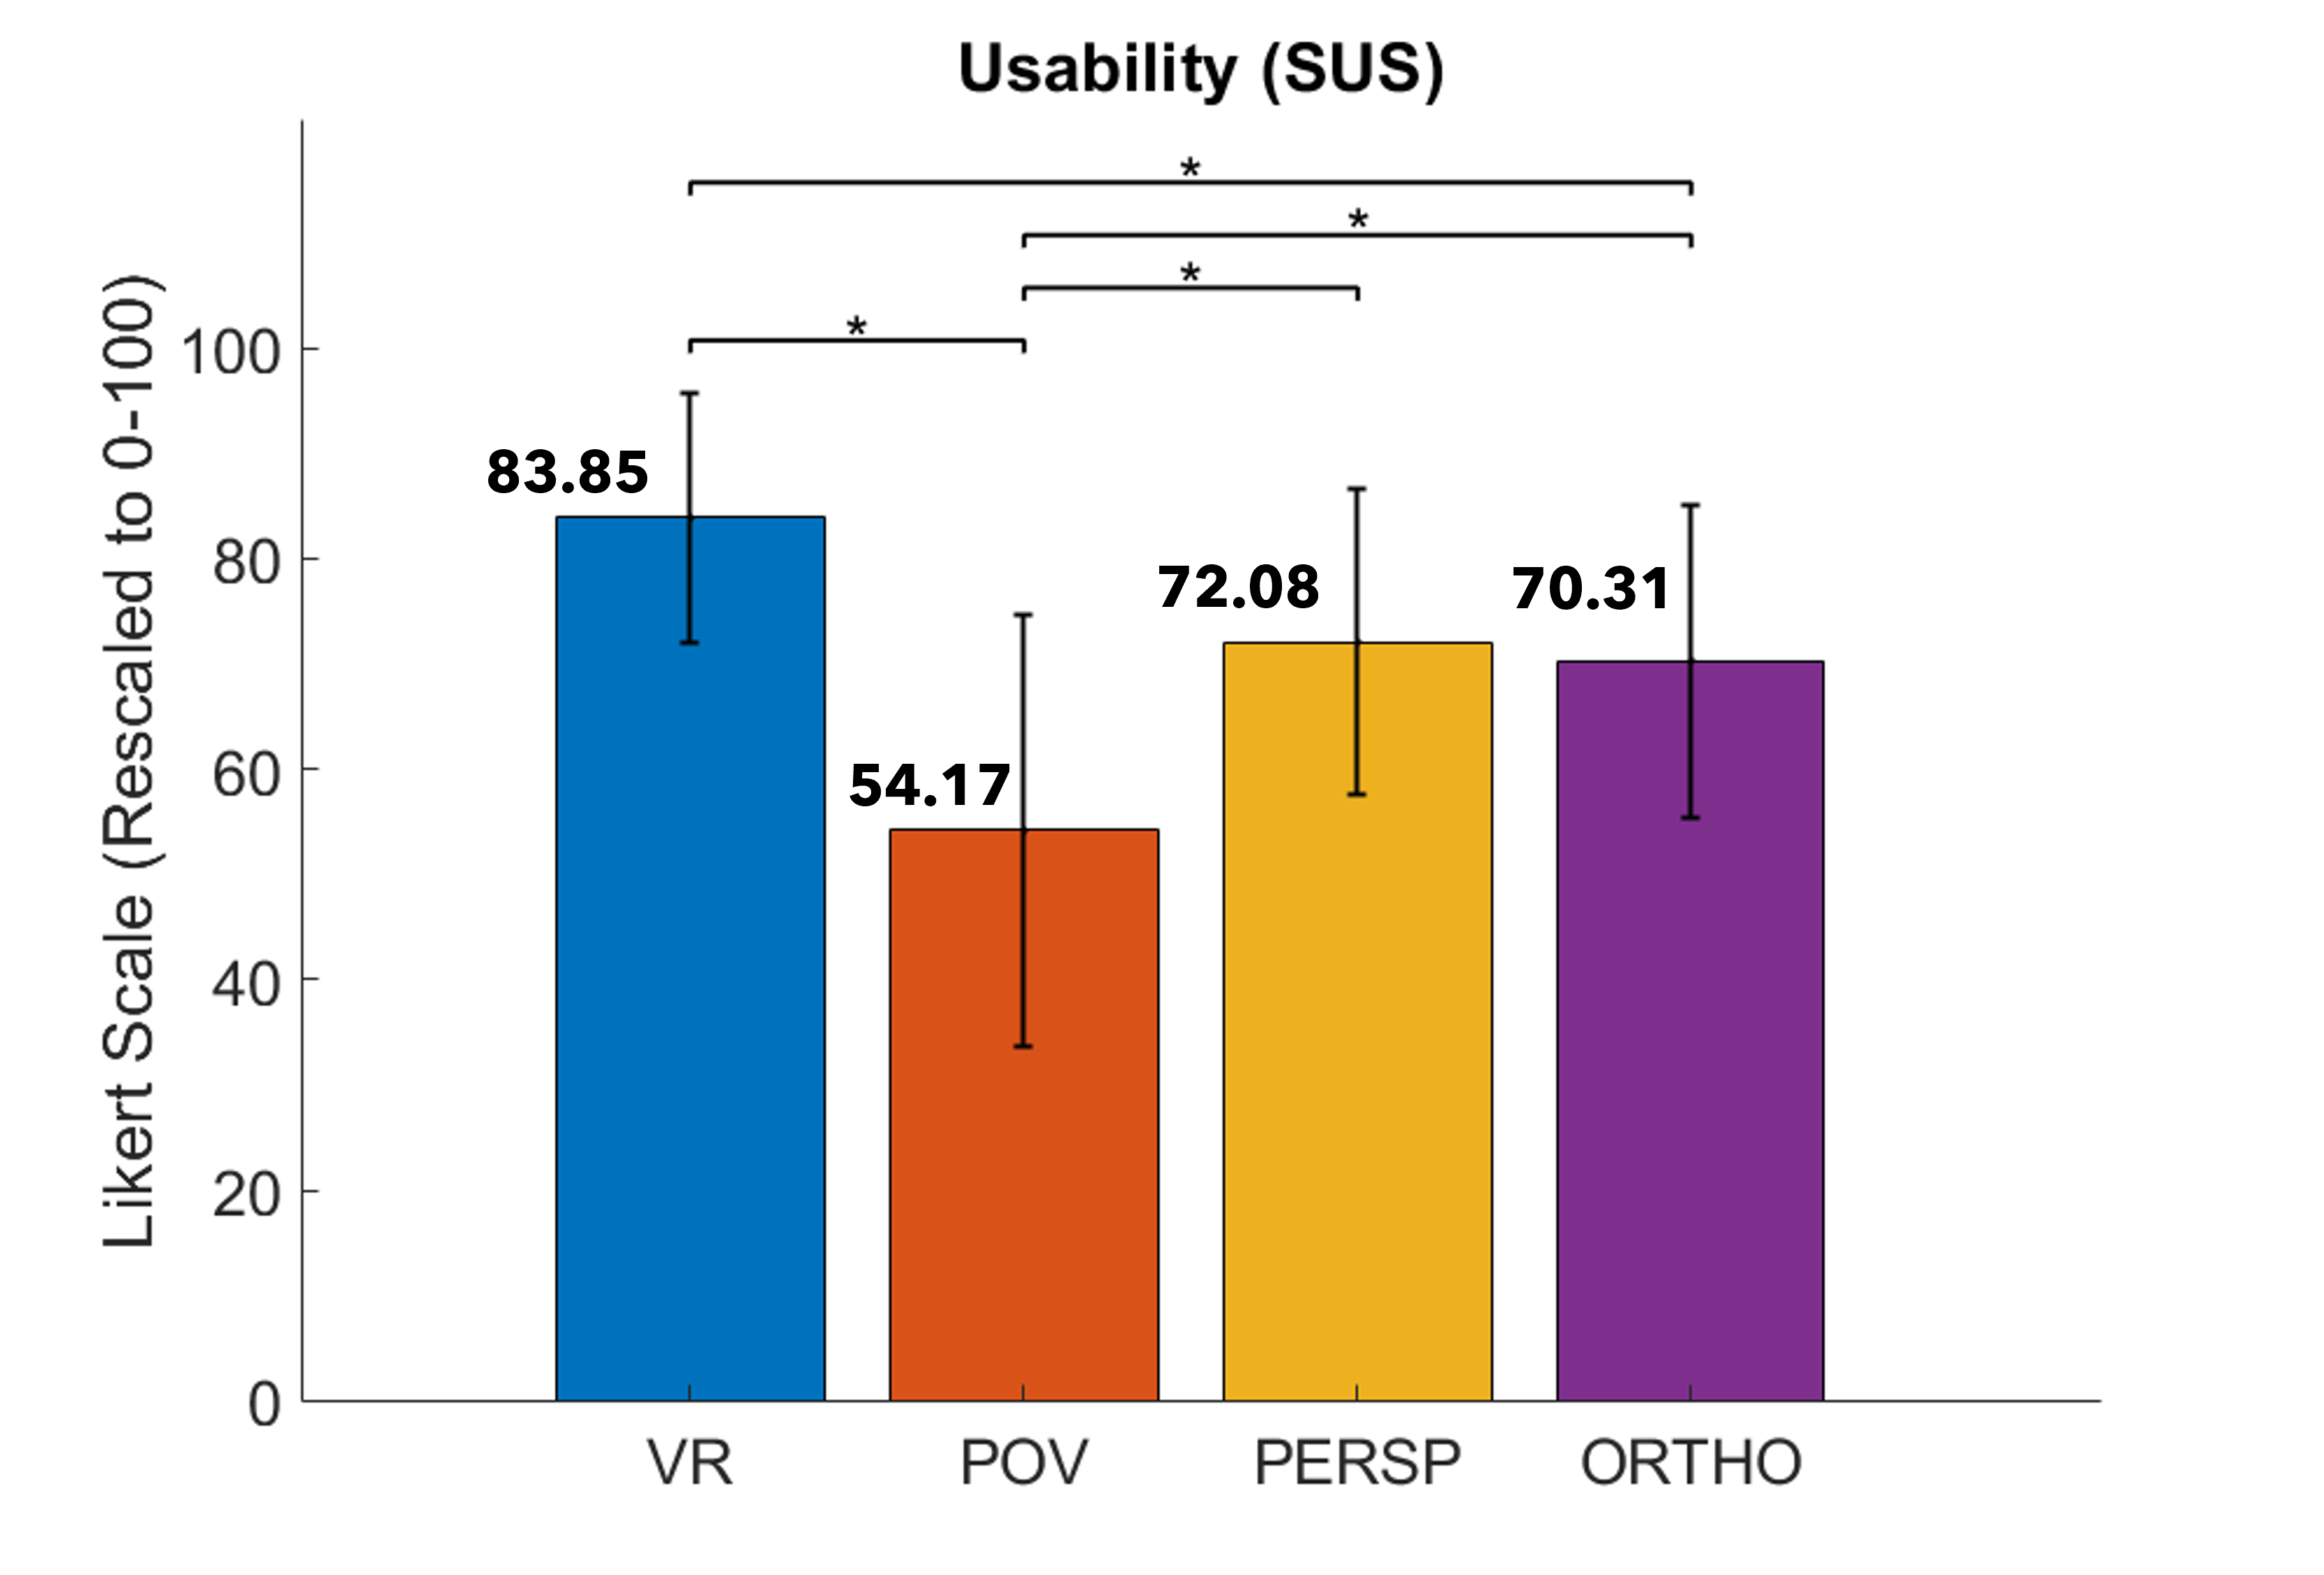
\includegraphics[width=\linewidth]{figures/VisualizationMod/Questionari/SUS.png}
	\end{columns}
	
	\citefooter{Pizzo et al., 2025}
\end{frame}

\begin{frame}{Study 3 Results: Cognitive Load}
	\begin{columns}[c]
		\column{0.3\textwidth}
		\begin{itemize}			
			\item VR vs.\ POV: statistically significant differences in physical demand, performance, and frustration sub-scales
			\item Significant also in overall NASA-TLX score
		\end{itemize}
		
		\column{0.7\textwidth}
		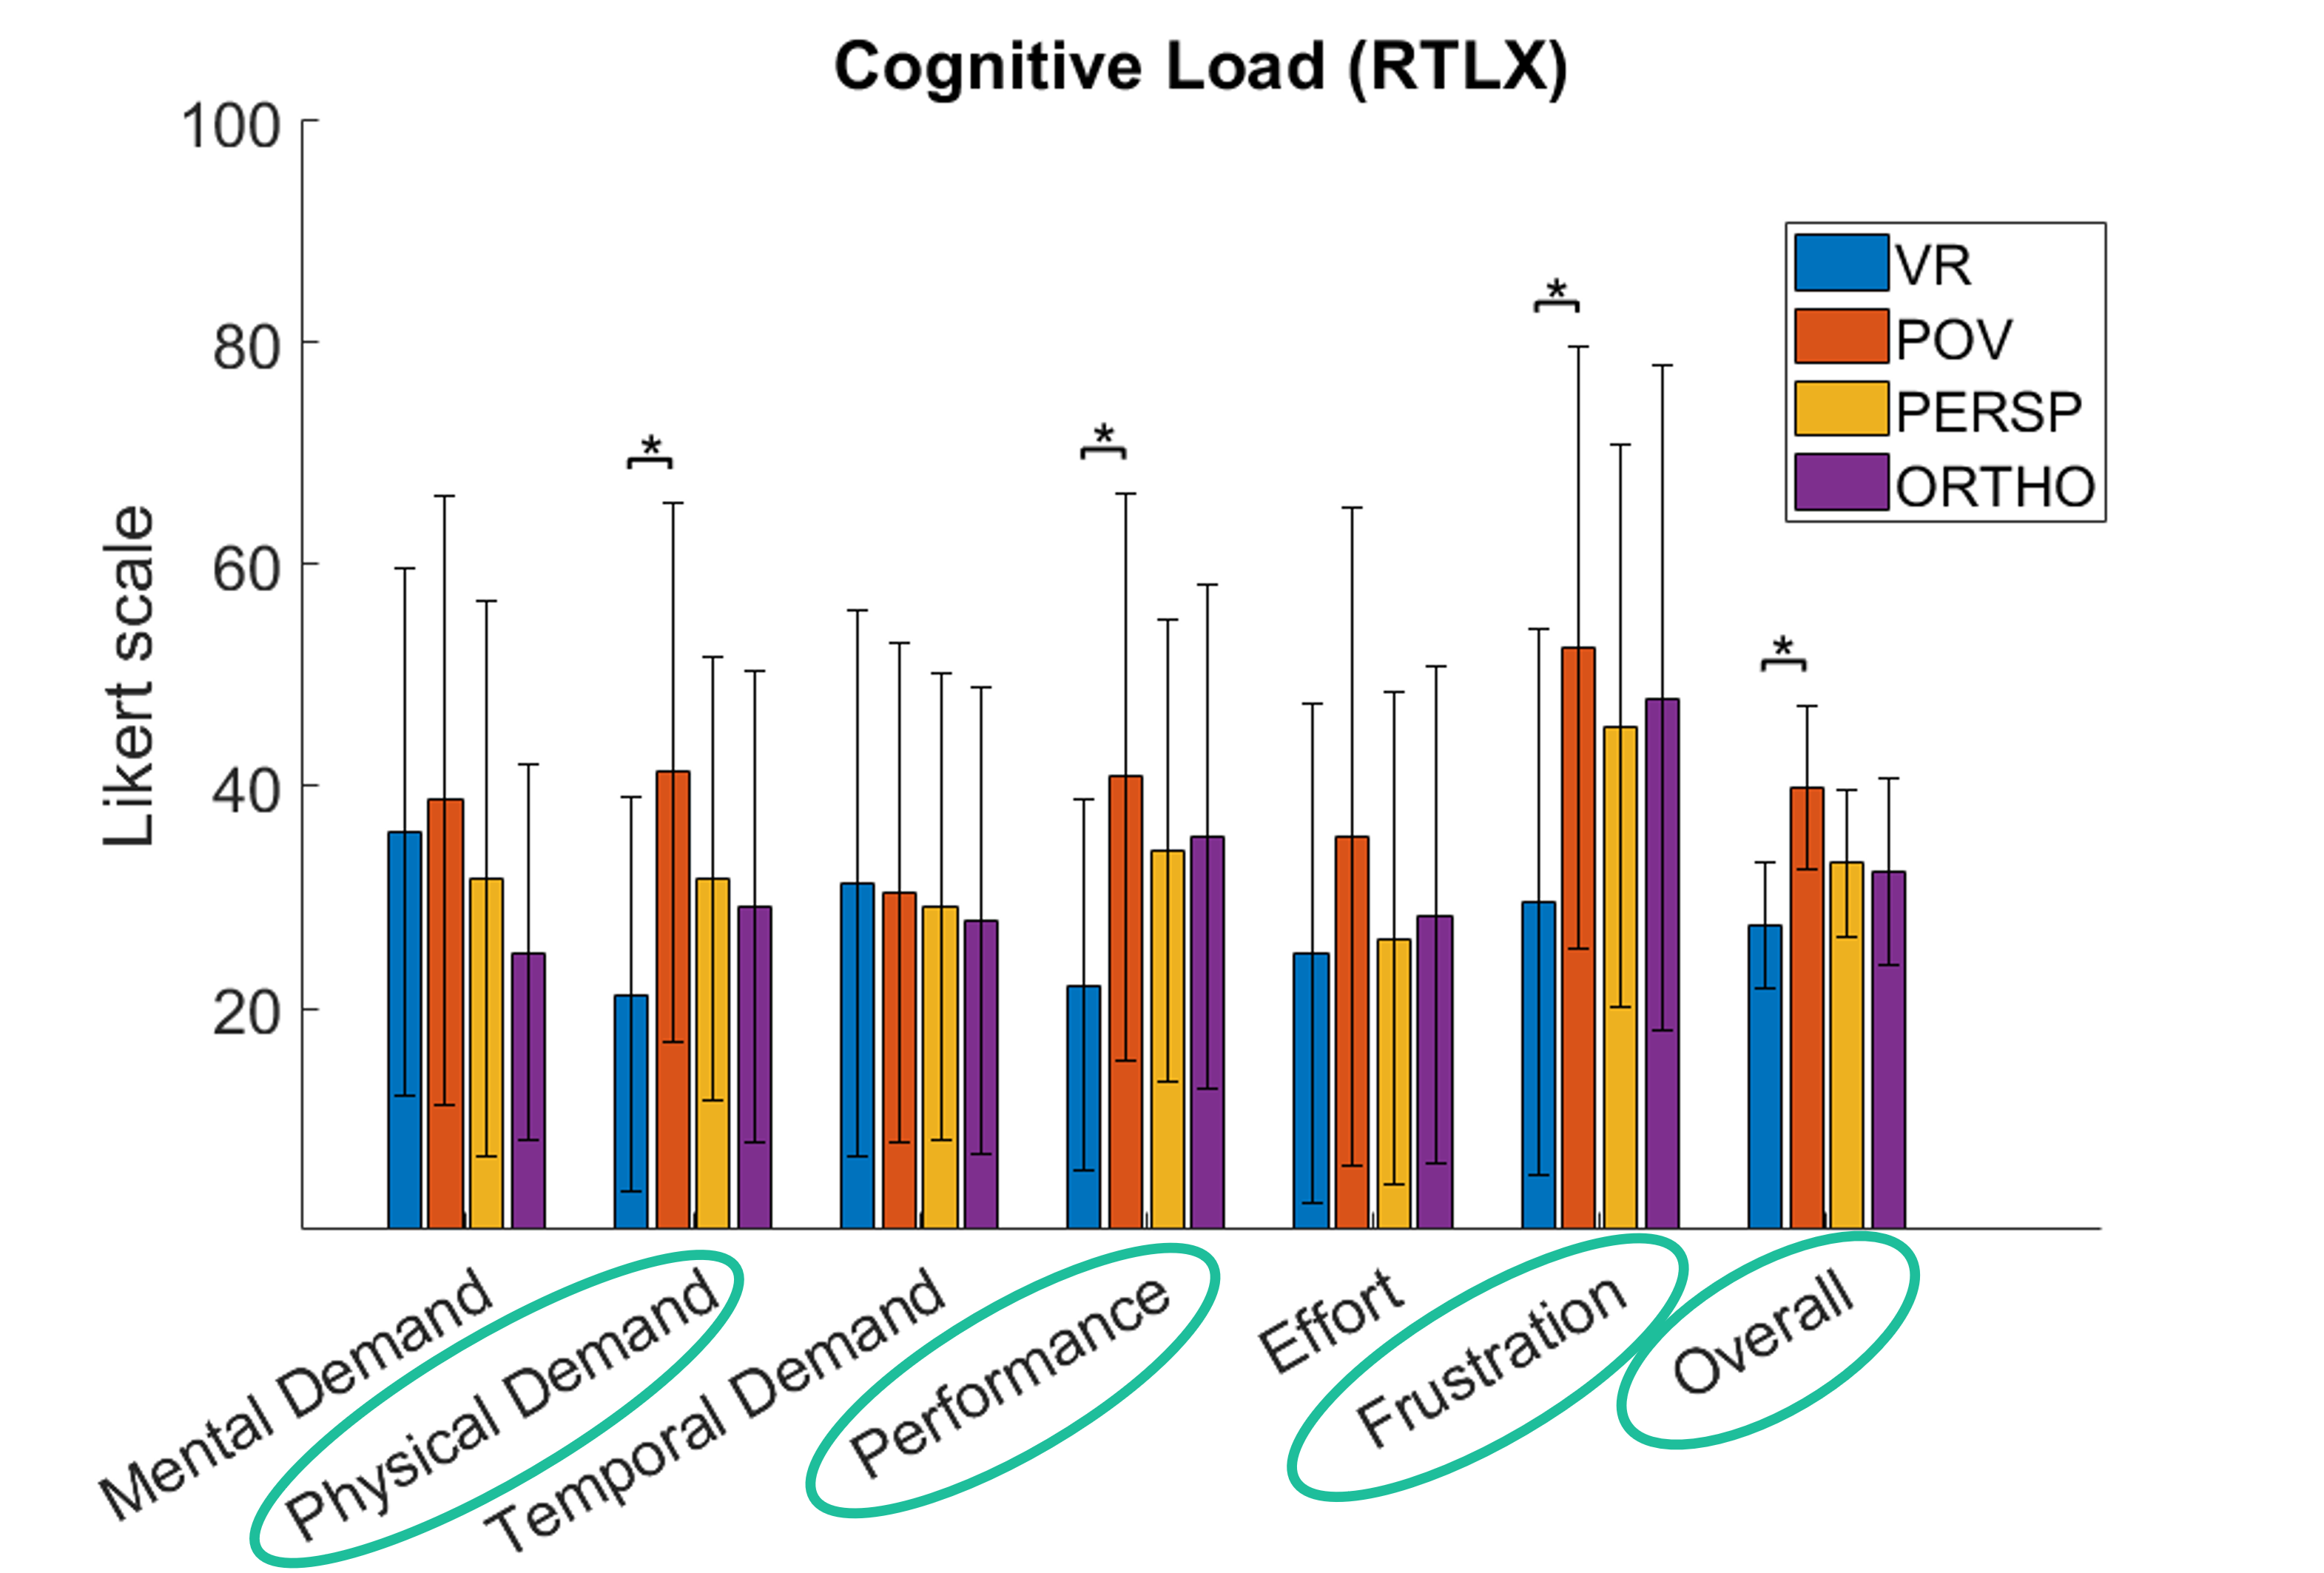
\includegraphics[width=\linewidth, height=0.8\textheight, keepaspectratio]{figures/VisualizationMod/Questionari/NASA.png}
	\end{columns}
	
	\citefooter{Pizzo et al., 2025}
\end{frame}

\begin{frame}{Study 3 Results: CMDT Performance}
	\begin{columns}[c]
		\column{0.3\textwidth}
		\textbf{\textcolor{gbAqua}{Key Findings}}
		\begin{itemize}
			\item \textbf{Miscounted cats} (pink): can be positive or negative; 
			\item \textbf{Untouched flowers} (green): inherently negative, reflects missed targets
			\item \textbf{Wrongly touched objects} (blue): always positive, incorrect touches relative to total displayed
		\end{itemize}
		
		\column{0.7\textwidth}
		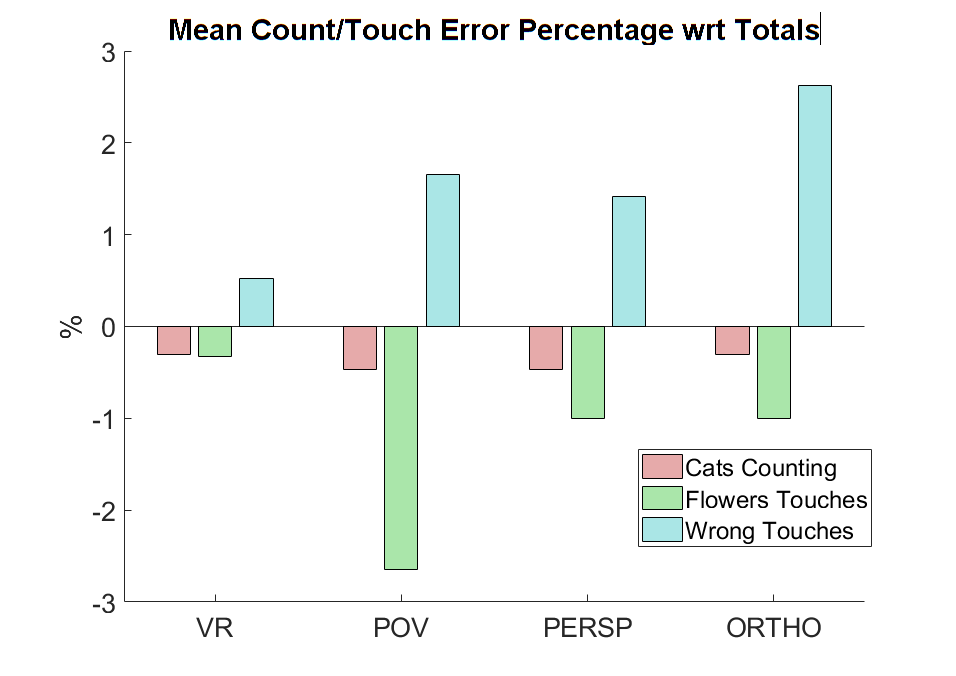
\includegraphics[width=\linewidth, height=0.8\textheight, keepaspectratio]{figures/VisualizationMod/ErroriPercentuali.png}
	\end{columns}
	
	\citefooter{Pizzo et al., 2025}
\end{frame}

\begin{frame}{Study 3: Discussion \& Conclusions}
	\begin{columns}[T]
		\column{0.5\textwidth}
		\textbf{\textcolor{gbAqua}{Hypotheses}}
		\begin{itemize}
			\item \textbf{H1 partially accepted}: VR significantly higher presence and usability than non-immersive; no significant differences in cognitive load
			\item \textbf{H2 rejected}: POV does NOT approximate IVR well. Significant differences in presence, usability, and cognitive load subscales
			\item \textbf{H3 accepted}: PERSP and ORTHO are comparable across all metrics
		\end{itemize}
		
		\column{0.5\textwidth}
		\textbf{\textcolor{gbAqua}{Implications}}
		
		When IVR is not feasible:
		\begin{enumerate}
			\item \textbf{First choice}: Fixed Perspective (PERSP). Consistently preferred, maintains 3D benefits.
			\item \textbf{Alternative}: Fixed Orthographic (ORTHO). Statistically comparable, viable when clinical requirements favor it.
		\end{enumerate}		
		
			\end{columns}
	
	\citefooter{Pizzo et al., 2025}
\end{frame}

\begin{frame}{Study 3: Limitations and Future Works}
	\textbf{\textcolor{gbAqua}{Limitation}}
	POV condition not ecologically implemented: the frustum follows the tracked head, causing projections inconsistent with real-world perception. Requires reimplementation with asymmetric frustum.
	\vspace{0.2cm}\\
	\textbf{\textcolor{gbAqua}{Open Questions}}
	\begin{itemize}
		\item \textbf{Ecological POV}: Reimplement using an asymmetric frustum with focal plane aligned to the real screen, so that virtual object projections behave consistently with real-world perception
		\item \textbf{Arm trajectories}: Study differences across modalities in users' reaching movements. Visualization may influence motor execution
		\item \textbf{Embodiment}: Evaluate the sense of body ownership across the four conditions
		\item Considering a more challenging CMDT
	\end{itemize}
	
	\citefooter{Pizzo et al., 2025}
\end{frame}

\begin{frame}[plain]
	\vfill
	\begin{center}
		{\large \textcolor{gbAqua}{\textbf{Contribution 3}}}
		
		\vspace{0.4cm}
		
		{\LARGE \textbf{Engagement and Effectiveness: Design Choices in Pediatric Rehabilitation}}
		
	\end{center}
	\vfill
\end{frame}


\begin{frame}{Fit4MedRob: Target Population and Clinical Challenges}
	\textbf{\textcolor{gbAqua}{Who}}
	
	Children with congenital or acquired neuromotor disorders, such as cerebral palsy (CP) or acquired brain injury (ABI)
	
	\vspace{0.3cm}
	
	\textbf{\textcolor{gbAqua}{Challenges}}
	
	\begin{itemize}
		\item Widely varying residual motor abilities
		\item Limited tolerance for frustration
		\item Strong need for intrinsically motivating activities to sustain the repetition required for neuroplasticity and motor learning
	\end{itemize}
	
	\vspace{0.3cm}
	
	\textbf{\textcolor{gbAqua}{Standard Controllers Are Ill Suited}}
	
	Not designed for children, no postural support, lack the ergonomic and therapeutic specificity required for meaningful motor training
	
	\citefooter{Alrashidi et al., 2023; Ravi et al., 2017; Levac et al., 2019}
\end{frame}

\begin{frame}{Exergames for Motor Learning}
	\textbf{\textcolor{gbAqua}{Exergames and Motor Learning}}
	
	\begin{itemize}
		\item Repetition of goal oriented tasks
		\item Immediate feedback
		\item Intrinsic motivation and sustained attention
	\end{itemize}
	
	\vspace{0.2cm}
	
	Multimodal feedback helps children understand if the movement is correct and supports motor control.
	
	\vspace{0.3cm}
	
	\textbf{\textcolor{gbAqua}{Clinical Evidence}}
	
	A systematic review and meta-analysis on XR assisted exergaming in children with cerebral palsy, \alert{45 studies, over 1500 participants}, confirmed significant improvements in global motor function and activities of daily living, and rated the technology as safe and well accepted
	
	\citefooter{Birckhead et al., 2019; Levac et al., 2019; Nossa et al., 2021; Tobaiqi et al., 2023}
\end{frame}

\begin{frame}{The Central Design Tension: Engagement vs Therapeutic Relevance}
	
	
	\begin{columns}[t]
		\column{0.48\textwidth}
		\textbf{\textcolor{gbAqua}{Motor Precision, Low Appeal and Engagement}}
		
		Many exergames in research prioritize motor precision over visual appeal, with task isolated interfaces that prioritize movement repetition over playfulness.
		
		\column{0.48\textwidth}
		\textbf{\textcolor{gbAqua}{High Appeal and Engagement, No Clinical Structure}}
		
		Wii Sports Resort in children with hemiplegic cerebral palsy: high engagement and adherence, but limited evidence of measurable clinical improvement
	\end{columns}
	
	\vspace{0.3cm}
	
	\alert{Engagement alone is not sufficient without a targeted therapeutic structure, but at the same time is required to sustain repetition and motivation, fundamental in motor therapy.}
	
	\citefooter{Biffi et al., 2017; Robertson et al., 2010; Bassano et al., 2022; Chiu et al., 2014}
\end{frame}

\begin{frame}{Beyond Standardization: The Case for Personalization}
	\textbf{\textcolor{gbAqua}{Standardization}}
	
	Uniform, evidence based protocols. Consistent delivery. A necessary step toward a reliable, adoptable clinical tool
	
	\vspace{0.3cm}
	
	\textbf{\textcolor{gbAqua}{Why Personalization Matters Most for This Population}}
	
	\begin{itemize}
		\item Each child has a distinct disorder severity, developmental stage, and evolving needs
		\item Configurable movements accommodate different impairment profiles
		\item Adjustable thresholds let therapists modulate difficulty and sensitivity
		\item Real time adaptive features prevent frustration, facilitate success
	\end{itemize}
	
	\citefooter{Felipe et al., 2020; Levitt et al., 2018; Figueiredo et al., 2025a, 2025b; Dominguez et al., 2020}
\end{frame}

\begin{frame}{From Theoretical Foundations to System Design}
	These considerations shaped the design of \textbf{ActivePaws}, a suite of three exergames.
	
	\vspace{0.3cm}
	
	\textbf{\textcolor{gbAqua}{Developed in Continuous Feedback Loop}} from biomedical engineers and therapists.
	
	\vspace{0.3cm}
	
	\textbf{\textcolor{gbAqua}{Semantic Coherence}}:	Movements are intuitively linked to their in game effect. Reinforces both engagement and therapeutic purpose.
	
	\vspace{0.3cm}
	
	\textbf{\textcolor{gbAqua}{User Centered Design}}
	\begin{itemize}
		\item Alternative gestures accommodate different impairment profiles
		\item Visually appealing layout yet simple enough to keep the motor task in focus
		\item Adjustable thresholds let therapists modulate game difficulty and sensitivity
		\item Real time adaptive features
	\end{itemize}
	
	\vspace{0.3cm}
	
\alert{Goal}: a system genuinely engaging and accessible, where gameplay demands therapeutically meaningful movement substaining motivation.
	
\end{frame}

\begin{frame}{The ActivePaws System}
	\small A non-immersive exergame suite controlled by the Playcuff wearable orthosis.
	
	\vspace{0.3cm}	
	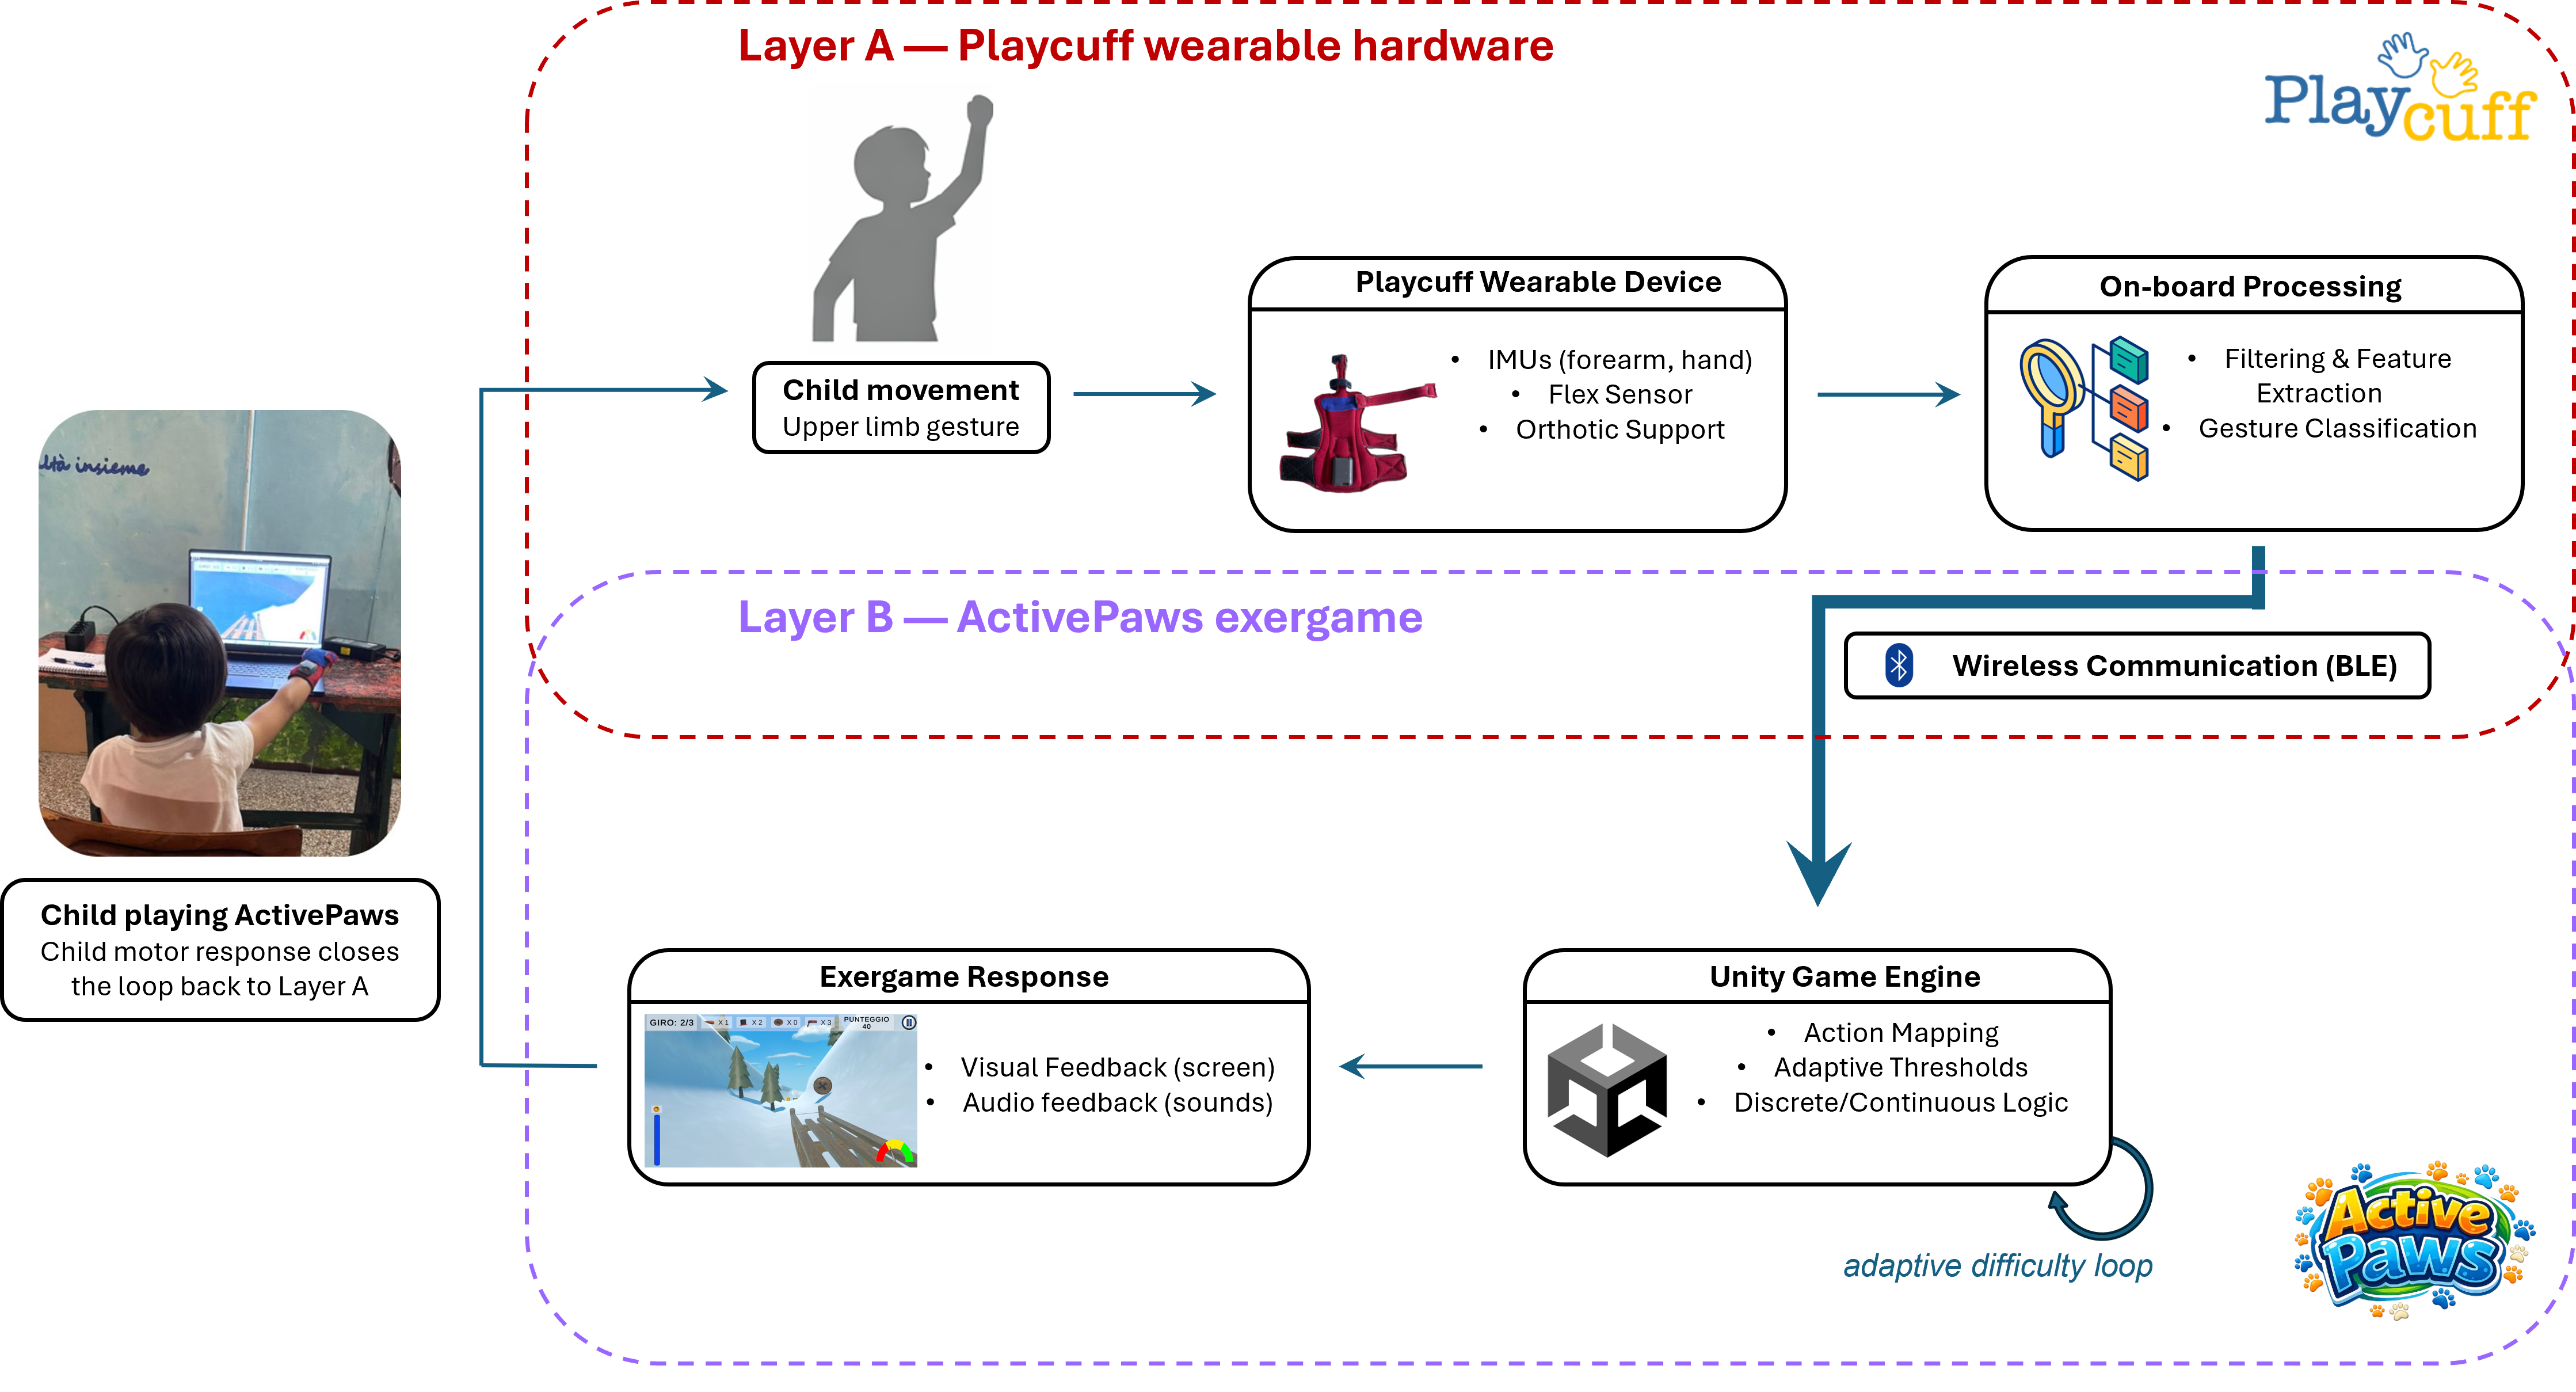
\includegraphics[width=0.8\linewidth]{figures/AP/AP_Scheme.png}	

\end{frame}

\begin{frame}[t]{The Playcuff Wristband}
	\begin{columns}[T]
		\column{0.55\textwidth}
		Soft wearable wrist orthosis developed at CNR-ICMATE for pediatric upper limb rehabilitation
		
		\vspace{0.1cm}
		
		\begin{itemize}
	\item \textbf{Postural support} and \textbf{real time gesture classification} for wireless (Bluetooth) game control
	\item Worn rather than held, no grip required
	\item Sensing: two IMUs (forearm, hand) plus a flex sensor to detect hand closing
	\item Firmware classifies gestures at 40 Hz
	\item Unity side: sliding window thresholds tracking \textbf{presence count} or \textbf{cumulative intensity}, tuned with the clinical team
\end{itemize}
		
		\column{0.45\textwidth}
		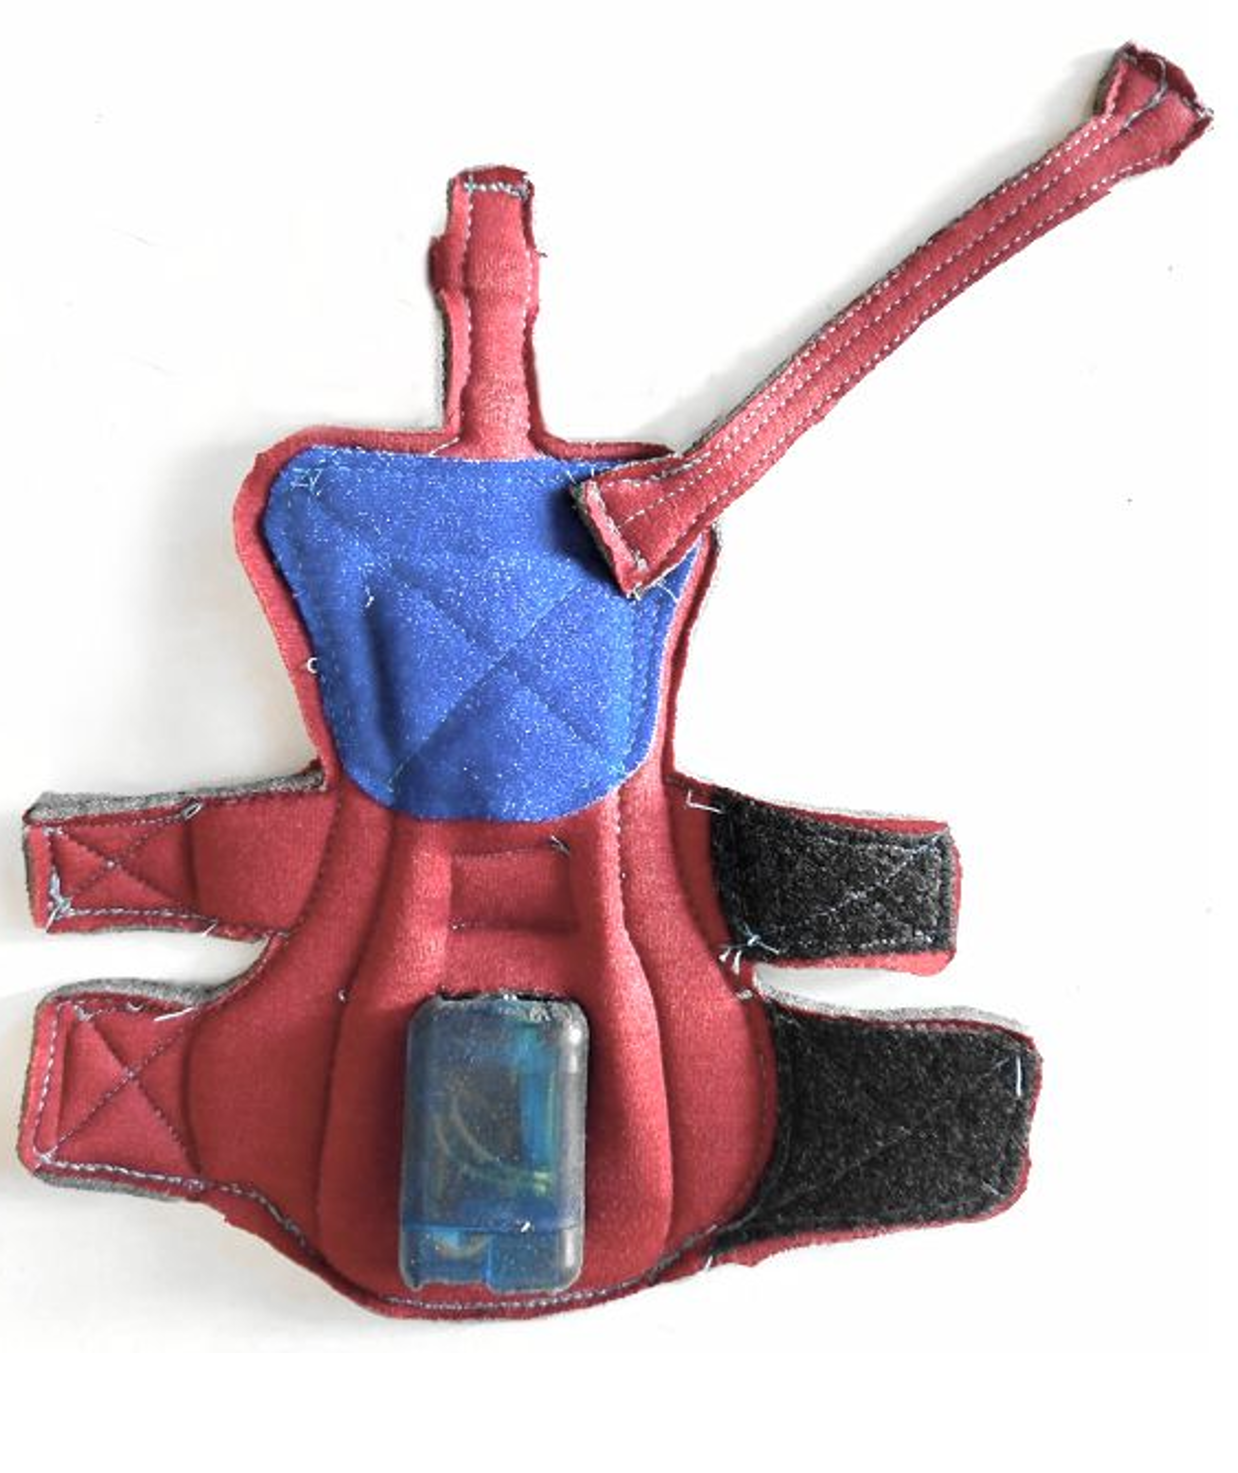
\includegraphics[width=\linewidth]{figures/AP/Playcuff.png}
	\end{columns}
	
	\citefooter{Lazzari et al., 2026}
\end{frame}


\begin{frame}{ActivePaws: Session Flow}
	\begin{columns}[T]
		\column{0.52\textwidth}
		\centering
		\begin{adjustbox}{max width=\linewidth, max totalheight=0.78\textheight}
		\begin{tikzpicture}[
			node distance=0.3cm,
			every node/.style={rectangle, rounded corners, draw=gbAqua, thick,
				text width=6cm, align=center, minimum height=1cm, font=\small},
			arr/.style={-{Latex}, thick, gbAqua}
		]
			\node (n1) {\textbf{Launch and Setup} \\ {\footnotesize Device selected by size (S, M, L), battery and connection status shown. Patient data}};
			\node (n2) [below=of n1] {\textbf{Therapist Configuration} \\ {\footnotesize Movement mapping, calibration, game settings}};
			\node (n3) [below=of n2] {\textbf{Tutorial} \\ {\footnotesize Illustrated intro, guided gesture practice}};
			\node (n4) [below=of n3] {\textbf{Gameplay Session} \\ {\footnotesize Child plays the selected level}};
			\node (n5) [below=of n4] {\textbf{Data Logging} \\ {\footnotesize Continuous JSON logging, organized by patient, game, and level. Game events and wristband classification}};
			\draw[arr] (n1) -- (n2);
			\draw[arr] (n2) -- (n3);
			\draw[arr] (n3) -- (n4);
			\draw[arr] (n4) -- (n5);
		\end{tikzpicture}
		\end{adjustbox}
		
		
\column{0.46\textwidth}
\centering
\begin{adjustbox}{max width=\linewidth, max totalheight=0.9\textheight}
\setlength{\tabcolsep}{3pt}
\renewcommand{\arraystretch}{1}
\newcolumntype{L}{>{\centering\arraybackslash}m{0.5cm}}
\newcolumntype{I}{>{\centering\arraybackslash}m{3.9cm}}
\begin{tabular}{L I I}
	\rotatebox[origin=c]{90}{\parbox{1.4cm}{\centering\footnotesize\textbf{Launch}}} &
	
\includegraphics[width=3.9cm]{figures/AP/schema/si.png} &
	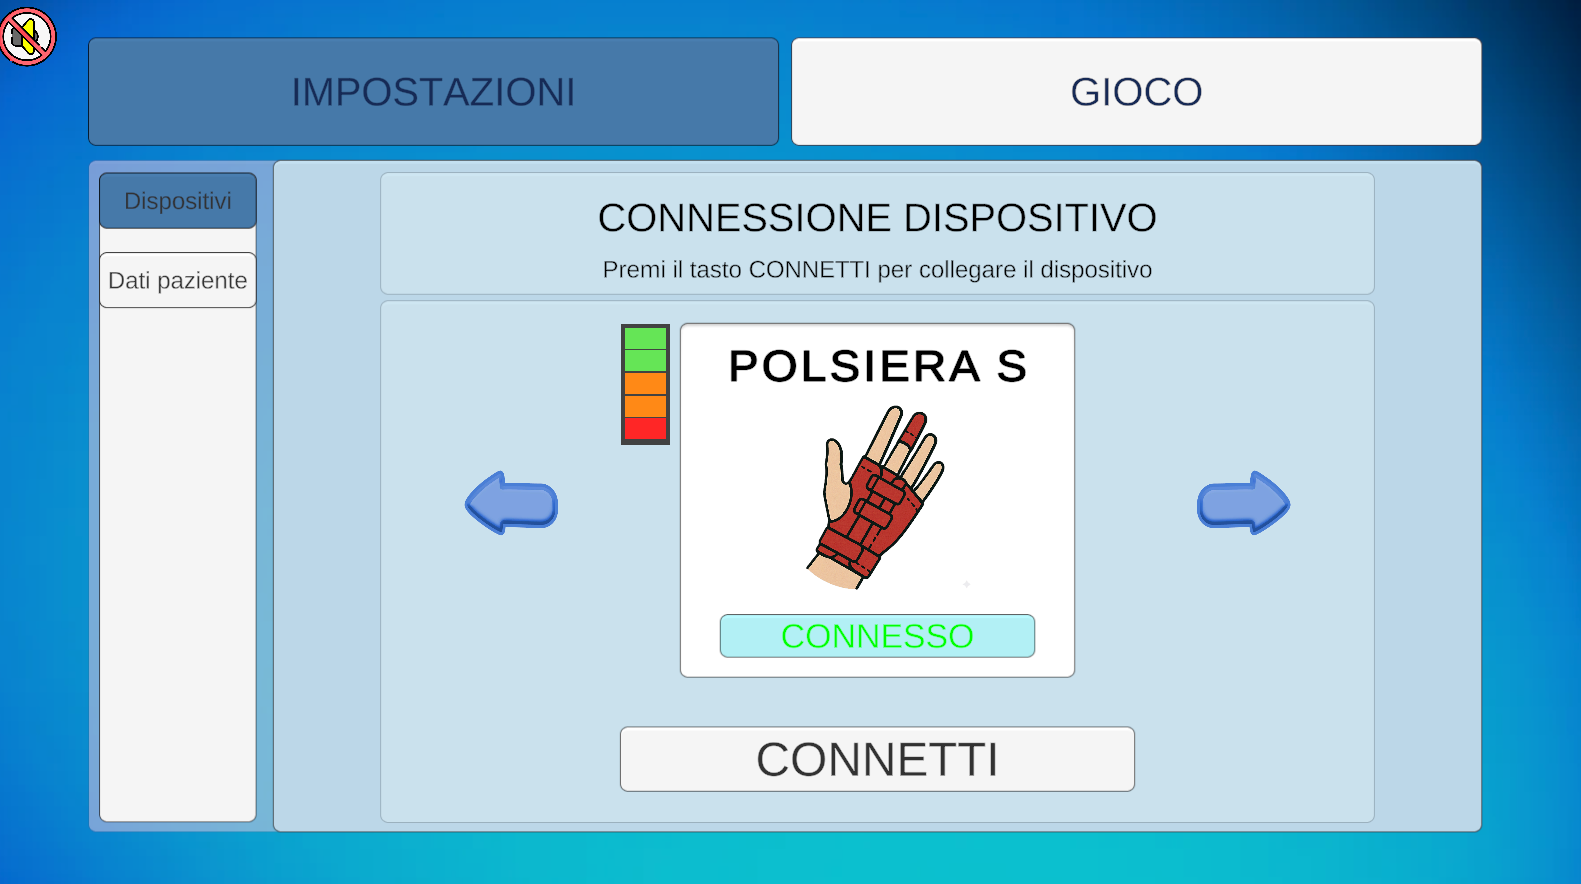
\includegraphics[width=3.9cm]{figures/AP/schema/bat.png} \\[0.15cm]
	
	\rotatebox[origin=c]{90}{\parbox{1.4cm}{\centering\footnotesize\textbf{Therapist\\Config.}}} &
	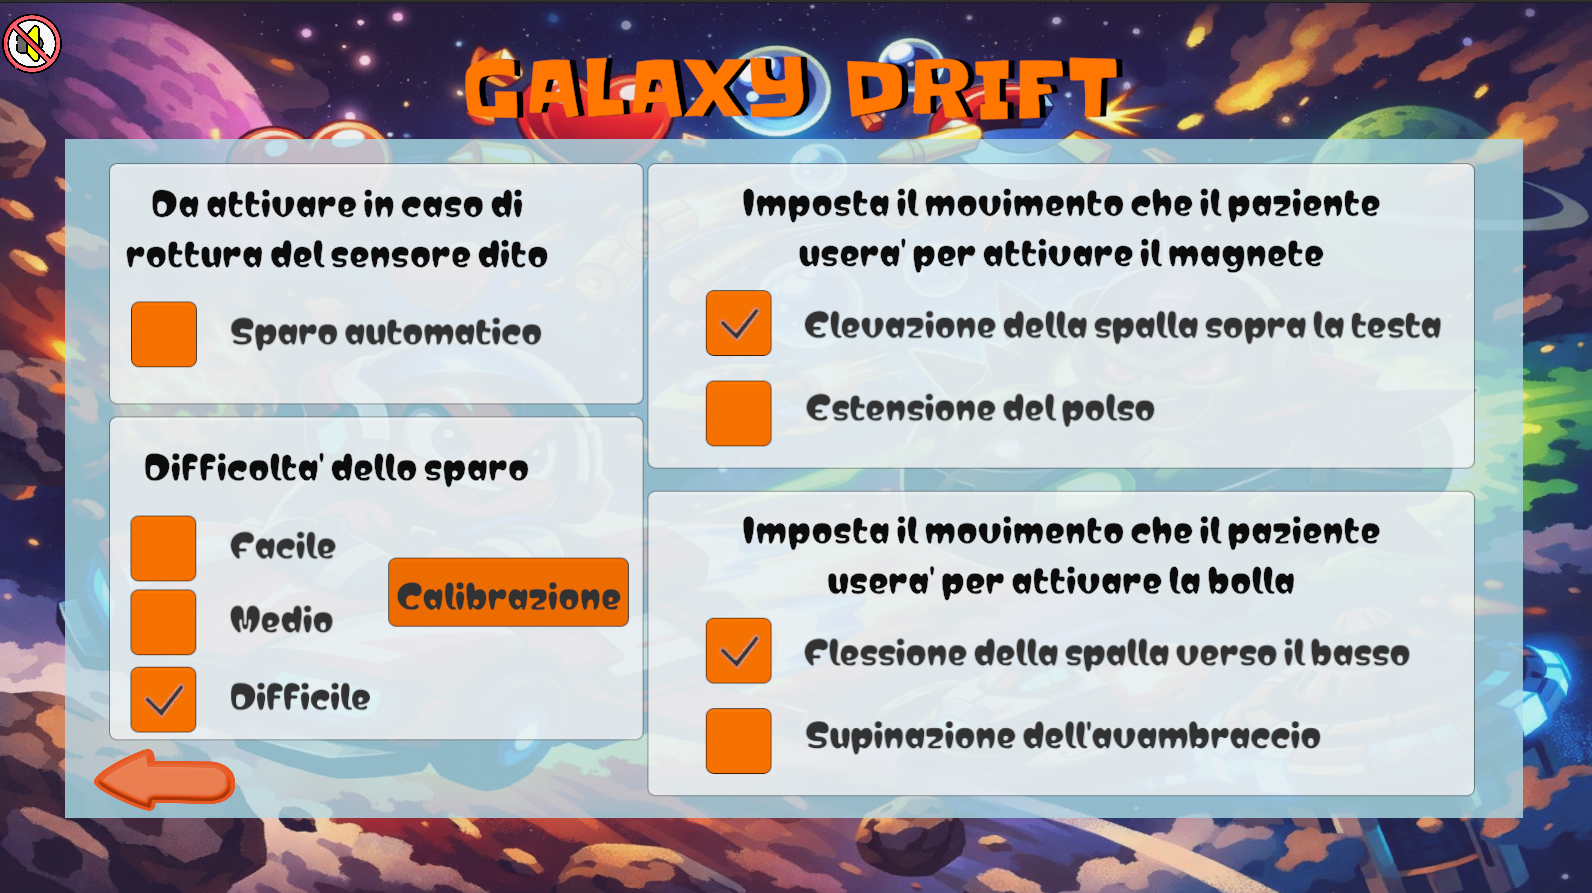
\includegraphics[width=3.9cm]{figures/AP/schema/mov.png} &
	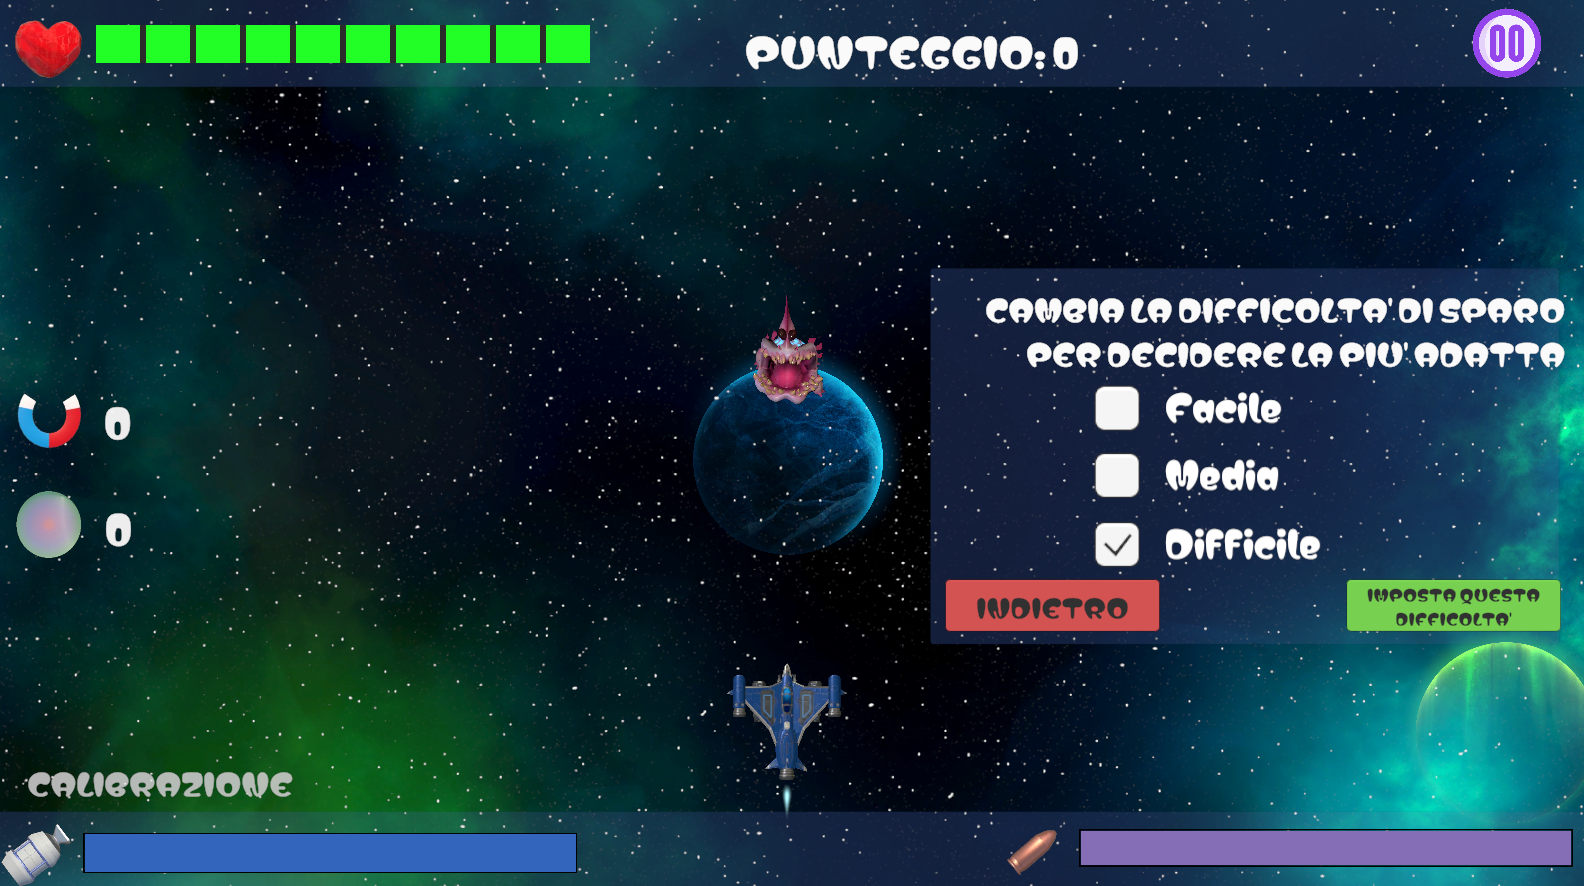
\includegraphics[width=3.9cm]{figures/AP/schema/cal.png} \\[0.15cm]
	
	\rotatebox[origin=c]{90}{\parbox{1.4cm}{\centering\footnotesize\textbf{Tutorial}}} &
	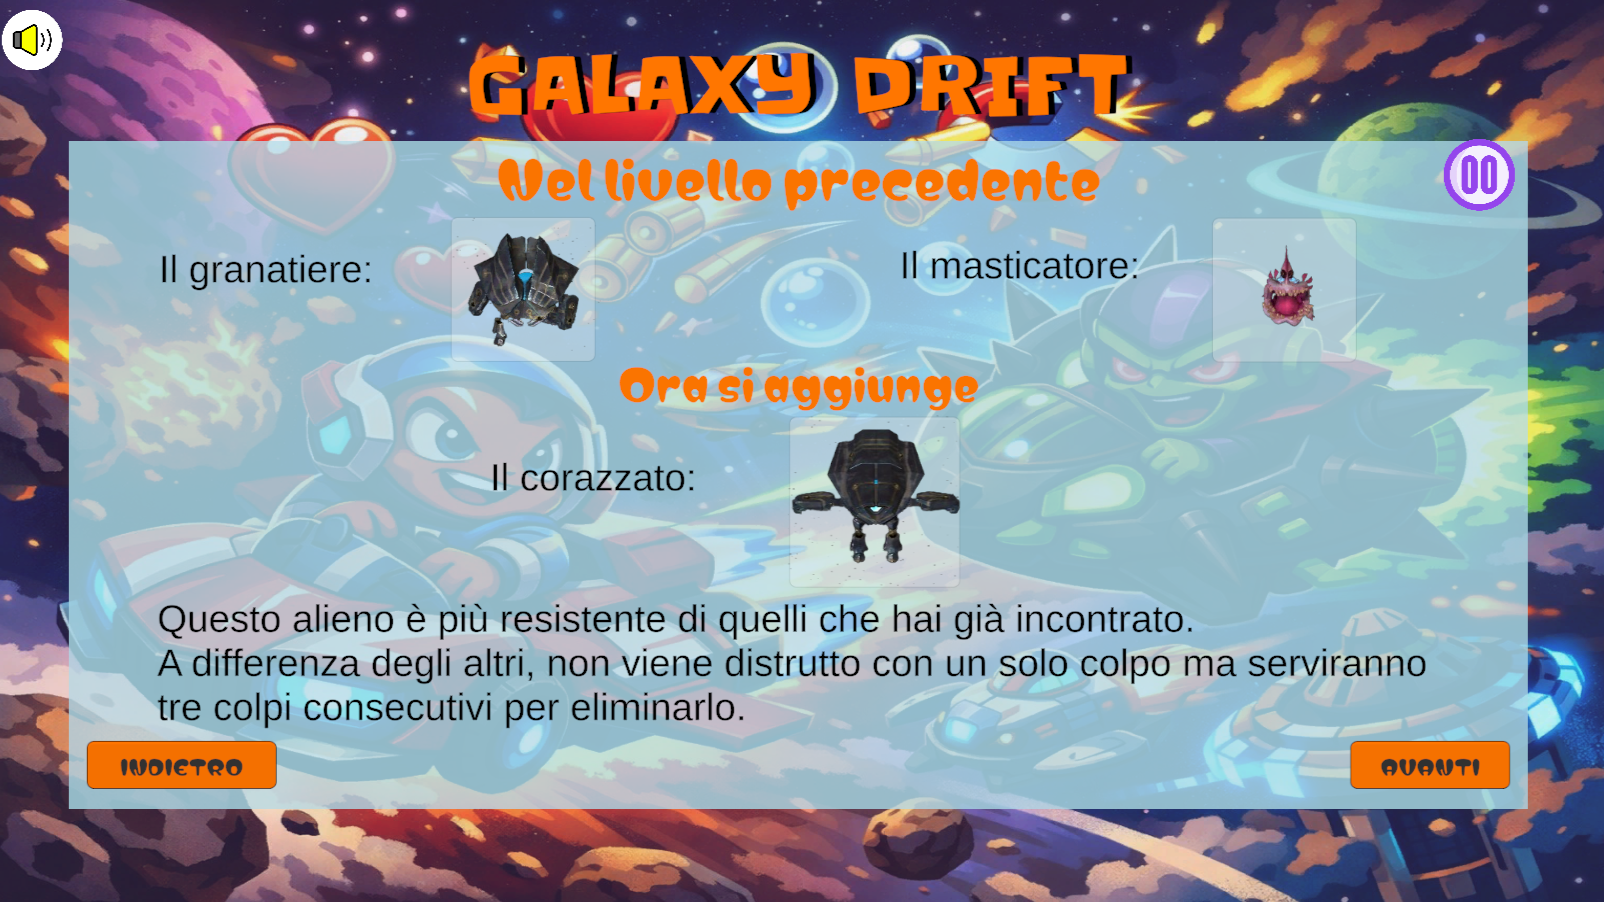
\includegraphics[width=3.9cm]{figures/AP/schema/gd.png} &
	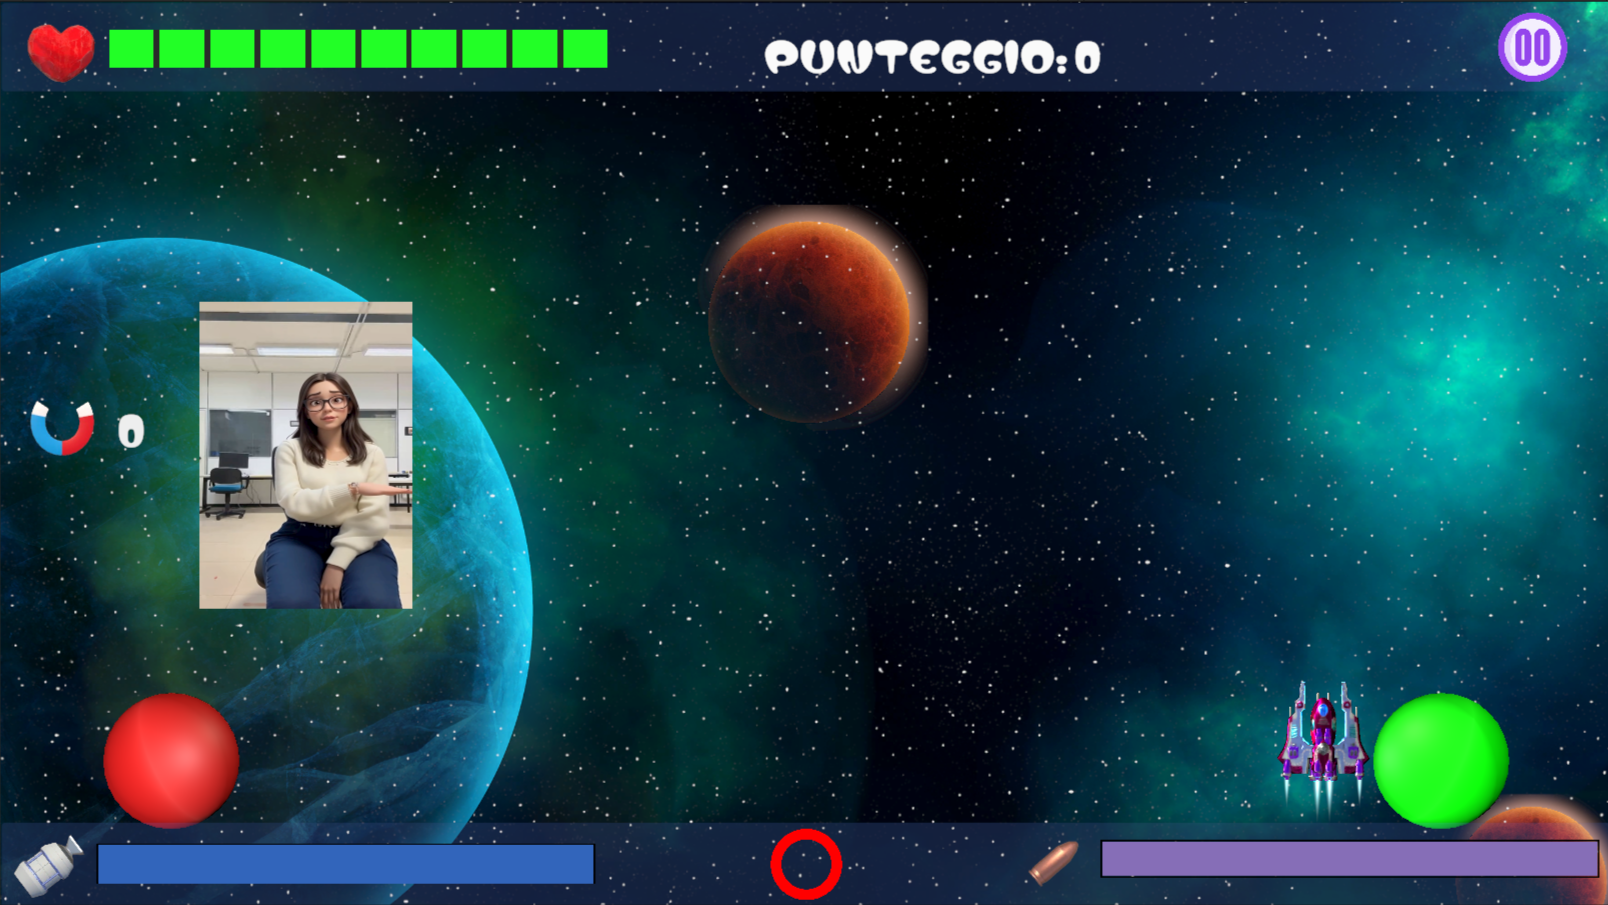
\includegraphics[width=3.9cm]{figures/AP/schema/gamegd.png} \\[0.15cm]
	
	\rotatebox[origin=c]{90}{\parbox{1.4cm}{\centering\footnotesize\textbf{Gameplay\\Session}}} &
	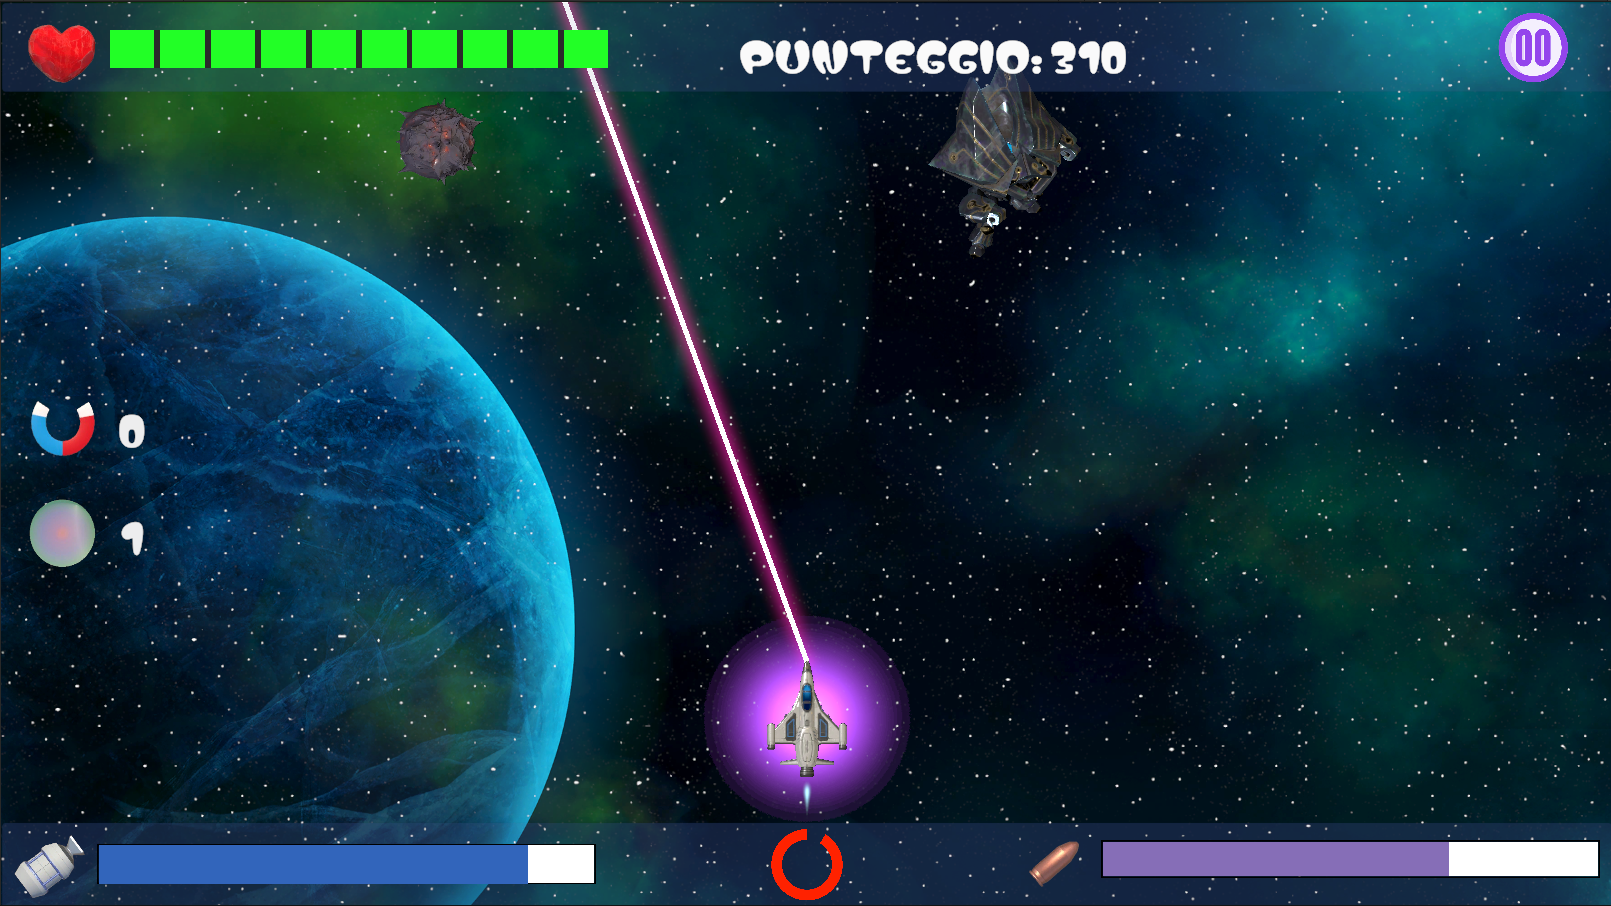
\includegraphics[width=3.9cm]{figures/AP/schema/3.png} &
	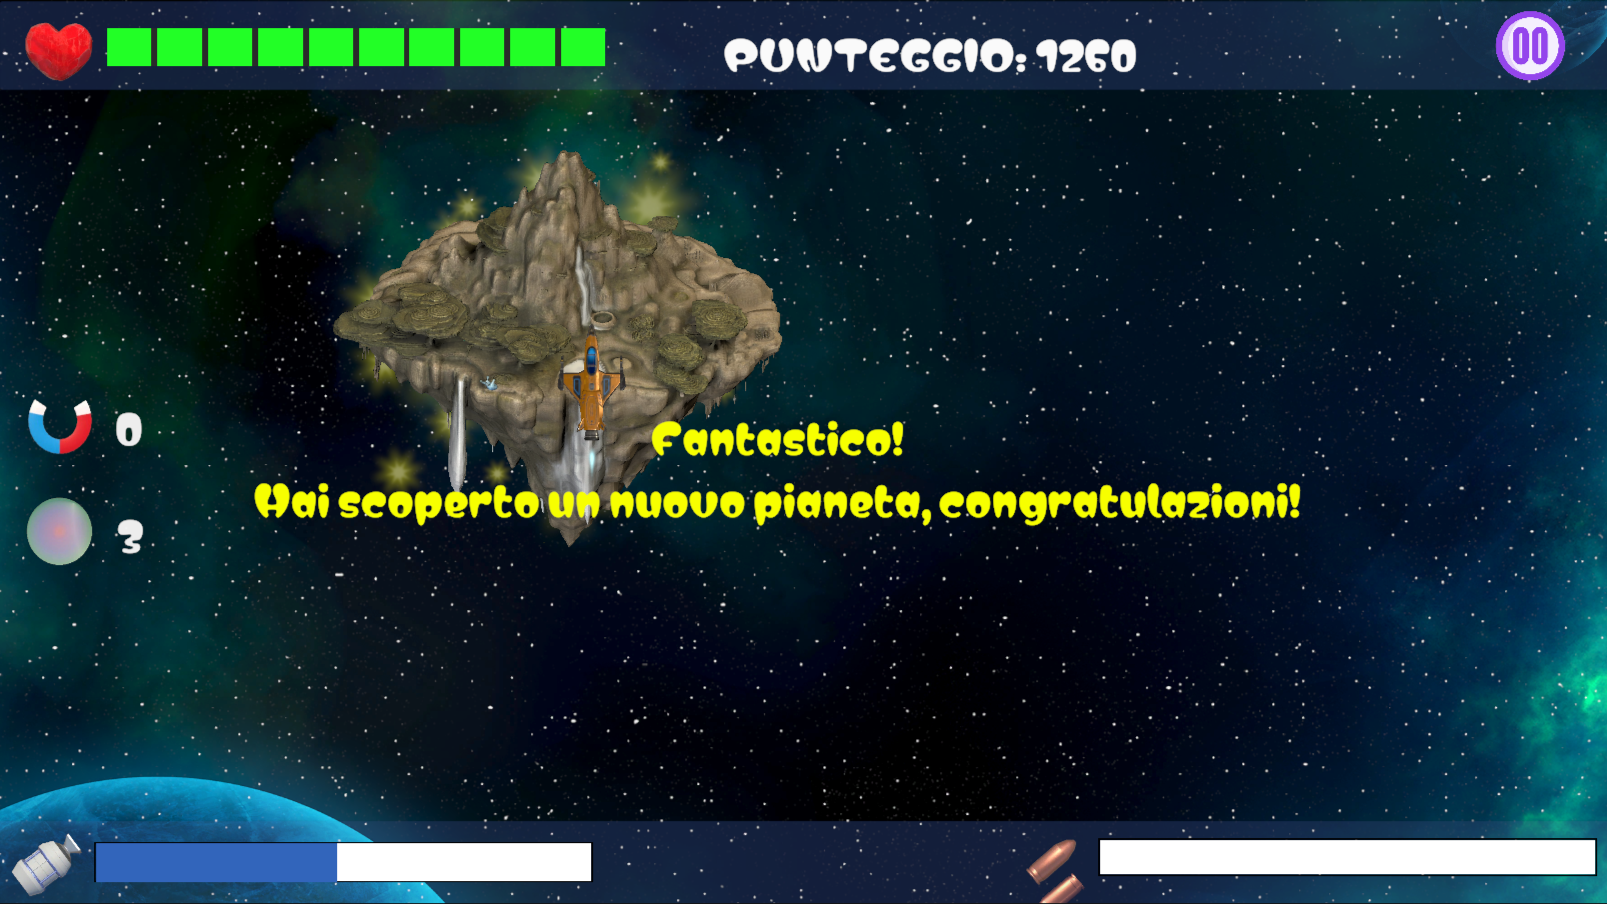
\includegraphics[width=3.9cm]{figures/AP/schema/4.png} \\
\end{tabular}
\end{adjustbox}
		
	\end{columns}
\end{frame}

\begin{frame}{Clinical Configuration and Tutorial}
	\begin{columns}[T]
		\column{0.5\textwidth}
		\textbf{\textcolor{gbAqua}{Movement Configuration}}
		
		Alternative gestures and adjustable intensity thresholds per action
		
		\vspace{0.2cm}
		
		\alert{Calibration scene}: To choose among the provided threshold a calibration scene has been recently added to choose the best one for each patient.
		
		\textbf{\textcolor{gbAqua}{Game Settings}}
		
		Different in-game features configurable to taylor training sessions and their difficulty, important to prevent frustration
		
		\column{0.5\textwidth}
		\textbf{\textcolor{gbAqua}{Two-Phase Tutorial}}
		

		\begin{itemize}
			\item Illustrated slides with voice over, no reading required
			\item Gated practical phase: gestures must be correctly performed before the game begins
			\item Adapts to configured alternative gestures
			\item Skippable at any point from the pause menu
		\end{itemize}
	\end{columns}
\end{frame}

\begin{frame}{ActivePaws: The Exergames}
	\begin{columns}[T]
		\column{0.32\textwidth}
		{\centering\color{gbAqua}\textbf{Swift Rescuer}\par}
		\vspace{2mm}
		\centering
		\begin{tikzpicture}
			\clip (0,0) rectangle (3.4,2.1);
			\node[anchor=center, inner sep=0] at (1.7,1.05)
				{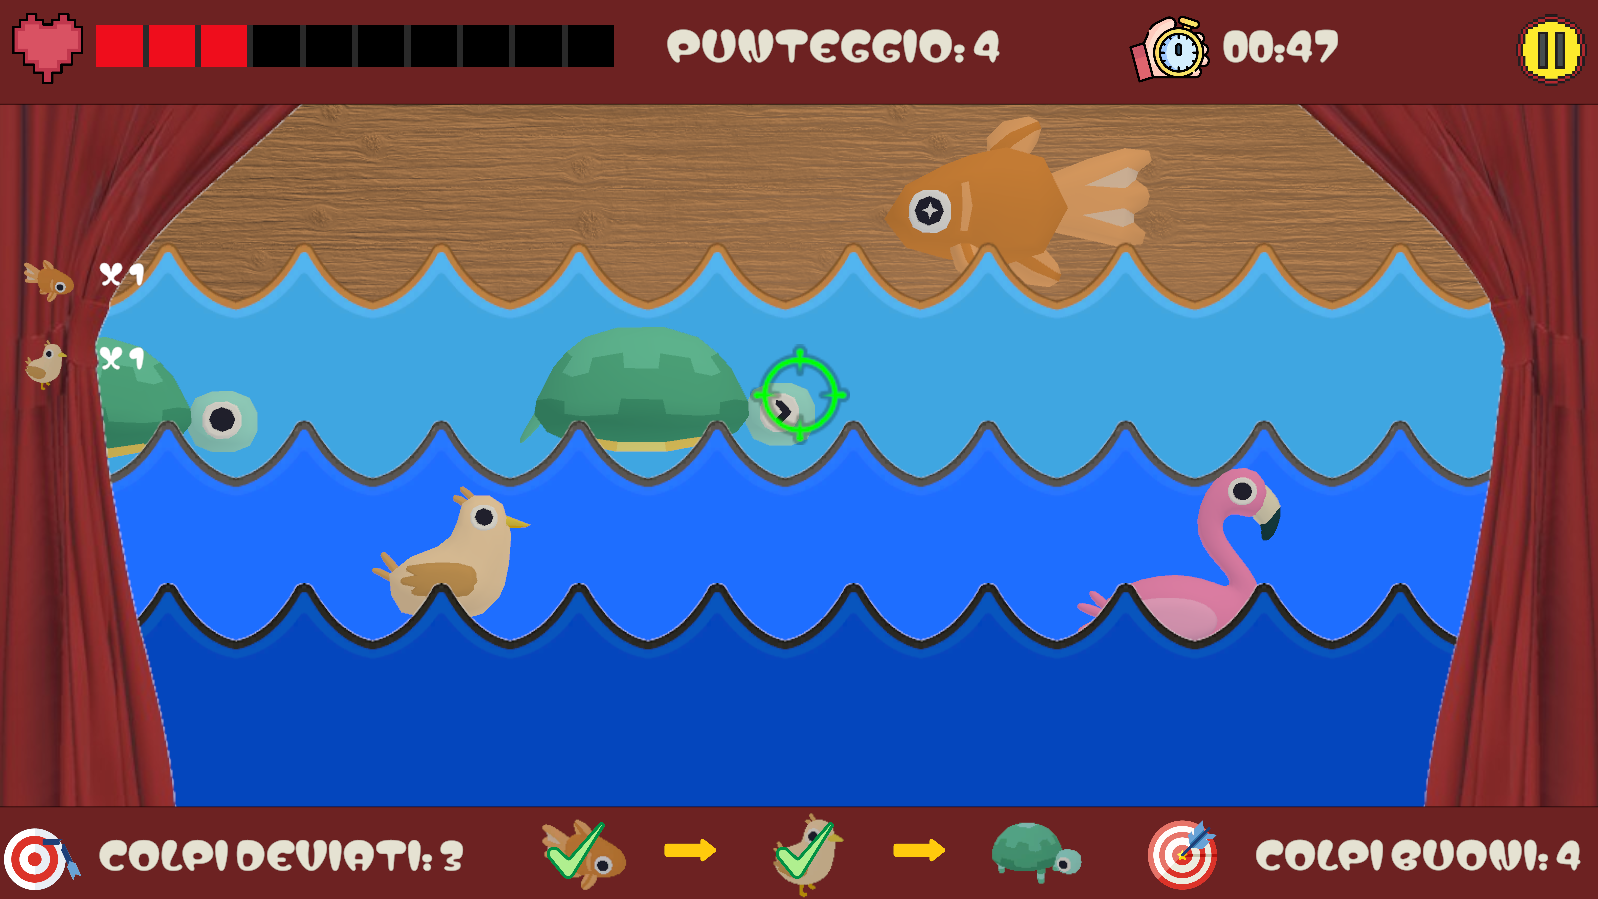
\includegraphics[height=2.1cm,width=3.4cm]{figures/AP/SR/4.png}};
		\end{tikzpicture}
		\vspace{2mm}
		{\footnotesize
		\begin{itemize}
			\item Orthographic shooting game. Player frees trapped animals
			\item Trains forearm stability and wrist extension
			\item Alternative gesture: hand opening via flex sensor
			\item Stability-to-shoot mapping. 
			\item 4 progressive levels. Last level adds a cognitive dimension
		\end{itemize}}
		
		\column{0.32\textwidth}
		{\centering\color{gbAqua}\textbf{Sledding Adventures}\par}
		\vspace{2mm}
		\centering
		\begin{tikzpicture}
			\clip (0,0) rectangle (3.4,2.1);
			\node[anchor=center, inner sep=0] at (1.7,1.05)
				{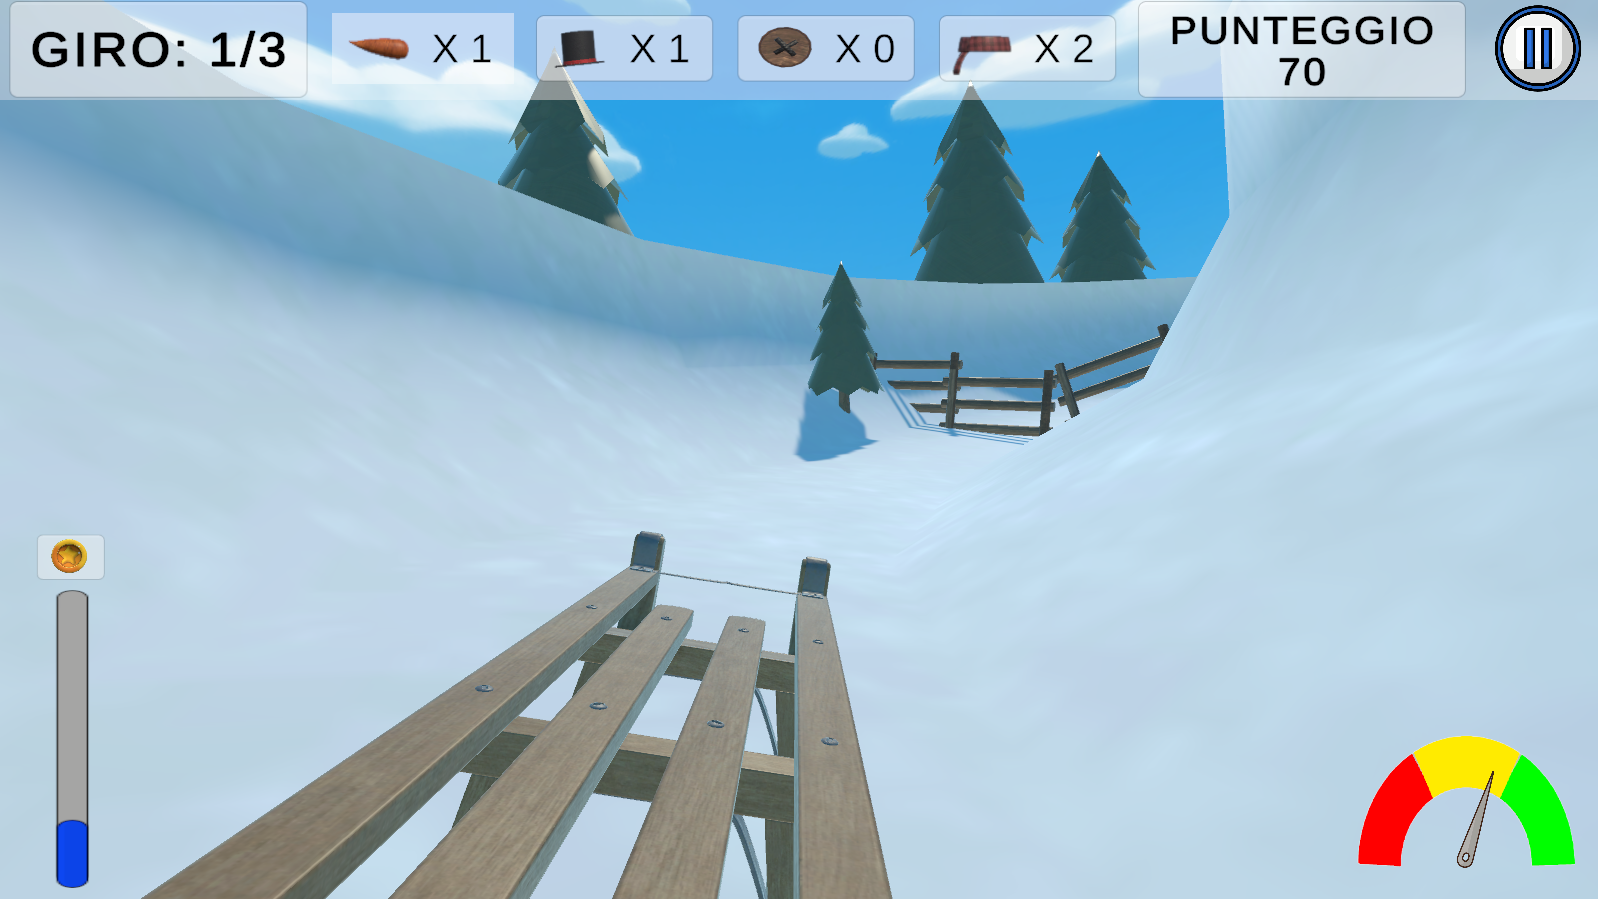
\includegraphics[height=2.1cm,width=3.4cm]{figures/AP/SA/4.png}};
		\end{tikzpicture}
		\vspace{2mm}
		{\footnotesize
		\begin{itemize}
			\item First-person sledding game. Collect items, avoid obstacles, complete laps
			\item Trains forearm pronosupination
			\item Higher levels add forearm elevation and hand closing
			\item Steering via pronation/supination, alternative: shoulder rotation
			\item 4 progressive levels
		\end{itemize}}
		
		\column{0.32\textwidth}
		{\centering\color{gbAqua}\textbf{Galaxy Drift}\par}
		\vspace{2mm}
		\centering
		\begin{tikzpicture}
			\clip (0,0) rectangle (3.4,2.1);
			\node[anchor=center, inner sep=0] at (1.7,1.05)
				{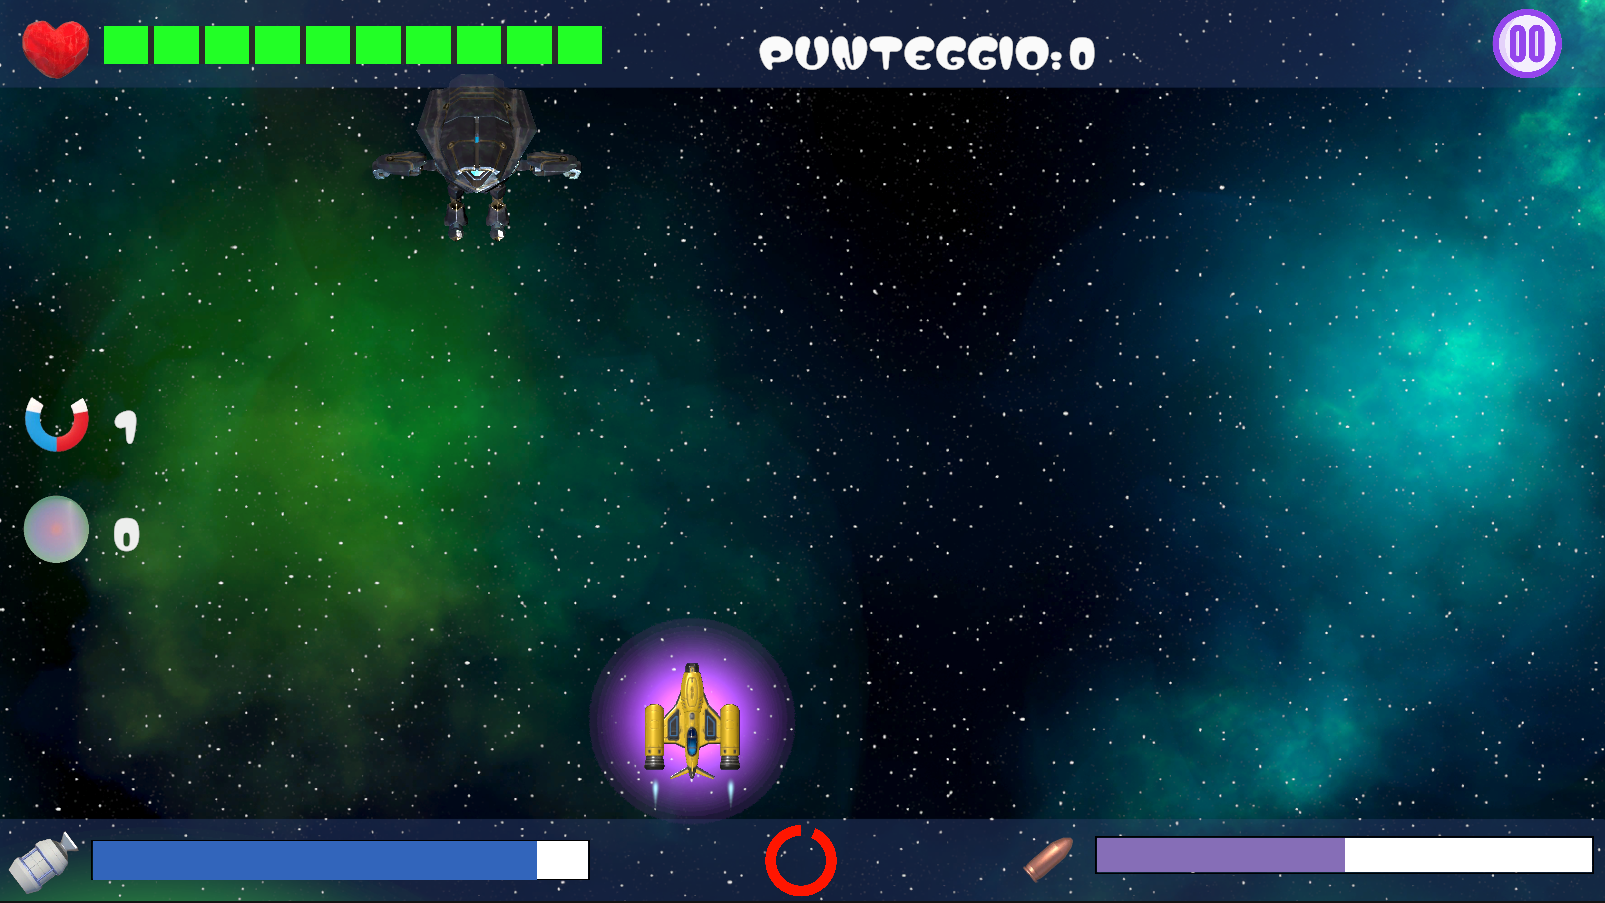
\includegraphics[height=2.1cm,width=3.4cm]{figures/AP/GD/2.png}};
		\end{tikzpicture}
		\vspace{2mm}
		{\footnotesize
		\begin{itemize}
			\item Top-down orthographic space game. Survive for a target time
			\item Trains shoulder rotation in the transverse plane
			\item Shooting via hand closing
			\item Manages lives, fuel, and ammunition. Power-ups: magnet, bubble
			\item 3 progressive levels
		\end{itemize}}
	\end{columns}
\end{frame}
\begin{frame}{ActivePaws in Action}
	
	\begin{center}
		\includegraphics[width=0.85\linewidth, height=0.55\textheight, keepaspectratio]{figures/intro/ap.png}\\[0.3cm]
		\href{https://drive.google.com/file/d/1a-kOVCpLSqV-s8Yc_942pxdX89hdeTBS/view?usp=sharing}{%
			\textcolor{gbAqua}{\textbf{$\blacktriangleright$ Video}}%
		}
	\end{center}	
\end{frame}

\begin{frame}{Study 4}
    \textbf{\textcolor{gbAqua}{ActivePaws and Playcuff: Pilot Evaluation of a Non-Immersive Exergame Suite Controlled by a Wearable Device}}
    
    \vspace{0.5cm}
    
    
        \small\textit{Based on:}
        
        \vspace{0.2cm}
        
        {\footnotesize M. Pizzo, et al., ``ActivePaws and Playcuff: Pilot Evaluation of a Non-Immersive Exergame Suite Controlled by a Wearable Device,'' IEEE ISMAR-Adjunct, 2025}
   
\end{frame}

\begin{frame}{Study 4: Goal and Methods}
	\textbf{\textcolor{gbAqua}{Goal}}
	
	Preliminary step toward clinical application, assessing two main aspects: children's \textbf{engagement} during gameplay, \textbf{usability} of the exergames
	
	\textbf{\textcolor{gbAqua}{Experiments}}
	
	12 participants, aged 6-14, 10 minutes of gameplay: Swift Rescuer and Sledding Adventures.
	
	\vspace{0.3cm}
	
	\begin{columns}[T]
		\begin{column}{0.5\textwidth}
			\textbf{\textcolor{gbAqua}{Participants}}
			\begin{itemize}
				\item \textbf{Healthy} children
				\item Most had gaming experience
				\item Tutorial at the beginning of each level
				\item \textbf{Single session} study
			\end{itemize}
		\end{column}
		\begin{column}{0.5\textwidth}
			\textbf{\textcolor{gbAqua}{Measures}}
			\begin{itemize}
				\item Questions on overall experience
				\item System Usability Scale for Kids (adapted)
				\item User Engagement Scale (adapted)
				\item Game performance logs
			\end{itemize}
		\end{column}
	\end{columns}
	
	\citefooter{Pizzo et al., IEEE ISMAR-Adjunct, 2025}
\end{frame}
\begin{frame}{Study 4: Post-Game Questionnaires Results}
	\begin{columns}[T]
		\begin{column}{0.48\textwidth}
			\textbf{\textcolor{gbAqua}{General questions}}
			\begin{itemize}
				\item SA was preferred
				\item SR more challenging but still engaging
				\item 91\% wanted to play again
			\end{itemize}
			
			\vspace{0.3cm}
			
			\textbf{\textcolor{gbAqua}{Usability}}
			\begin{itemize}
				\item $>$90\% no frustration
				\item $>$70\% would play on phone
				\item $>$50\% easy to use without help
				\item $>$80\% friends would learn quickly
			\end{itemize}
		\end{column}
		\begin{column}{0.48\textwidth}
			\centering
			\textbf{\textcolor{gbAqua}{User engagement questions}}
			
			\vspace{0.2cm}
			
			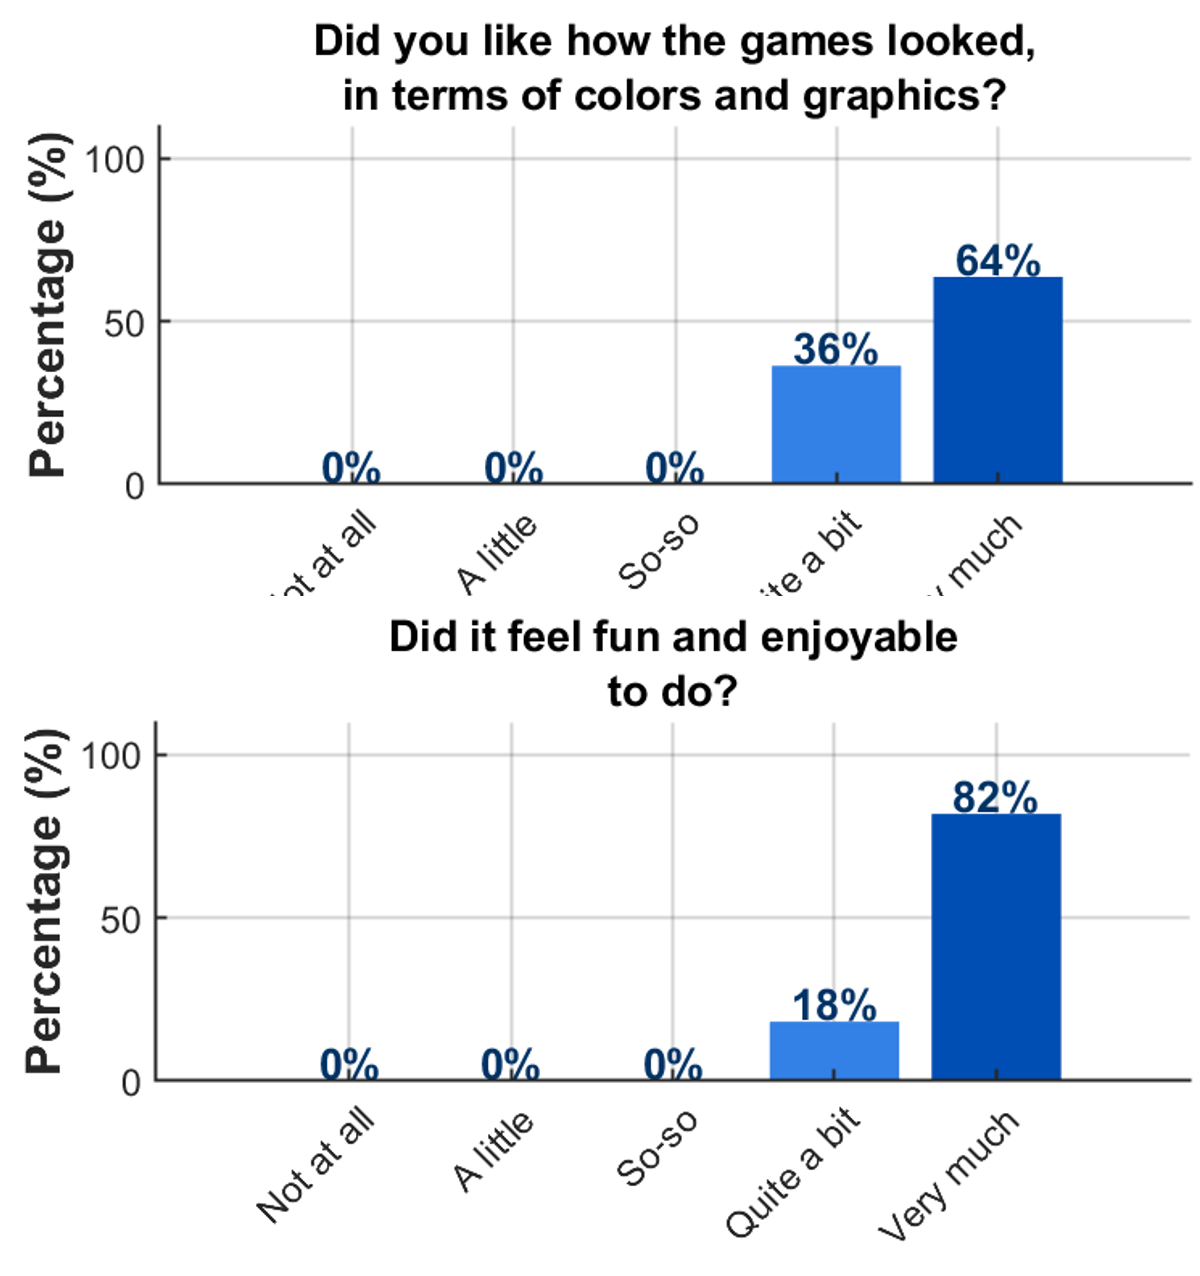
\includegraphics[width=0.7\textwidth]{figures/AP/plot.png}
			
			\vspace{0.2cm}
			
			\raggedright
			\begin{itemize}
				\item 100\% found the games fun, 100\% liked colors and graphics
				\item 81\% felt very or somewhat absorbed
			\end{itemize}
		\end{column}
	\end{columns}
	
	\citefooter{Pizzo et al., IEEE ISMAR-Adjunct, 2025}
\end{frame}

\begin{frame}{Study 4: Game Logs Results}
	\textbf{\textcolor{gbAqua}{Swift Rescuer}} (accuracy = shots hitting animals / total)
	
	\begin{itemize}
		\item \textbf{L1}: $0.69 \pm 0.21$ $\rightarrow$ high variability
		\item \textbf{L2}: $0.43 \pm 0.15$ $\rightarrow$ lower variability, more consistent
		\item \textbf{L3}: $0.47 \pm 0.10$ $\rightarrow$ only skilled players performed it
	\end{itemize}
	\textit{Obs.}: few row changes
	
	\vspace{0.3cm}
	
	\textbf{\textcolor{gbAqua}{Sledding Adventures}} (accuracy = collected snowman parts + coins / total)
	
	\begin{itemize}
		\item \textbf{L3 only}: $0.77 \pm 0.13$
	\end{itemize}
	\textit{Obs.}: consistent results across ages
	
	\citefooter{Pizzo et al., IEEE ISMAR-Adjunct, 2025}
\end{frame}


\begin{frame}{Study 4: Key Takeaways and Impact on Design}
	\textbf{\textcolor{gbAqua}{Key Takeaways}}
	
	\begin{itemize}
		\item Sledding Adventures was preferred over Swift Rescuer due to its game mechanics		
		\item Accuracy drop in Swift Rescuer across levels attributed to fixed gesture thresholds
		\item Wristband-based control proved effective across exergames
	\end{itemize}
	
	\vspace{0.3cm}
	
	\textbf{\textcolor{gbAqua}{Impact on Suite Design}}
	
	\begin{itemize}
		\item Motivated development of \textbf{Galaxy Drift} as a third exergame		
		\item Enabled \textbf{configurable gesture intensity thresholds} introduced calibration scene
		\item Introduced \textbf{adaptive features} for improved accessibility
		\item Tuned Swift Rescuer levels and introduced a dedicated \textbf{Level 4} for the ordered modality
	\end{itemize}
	
	
	\citefooter{Pizzo et al., IEEE ISMAR-Adjunct, 2025}
\end{frame}
\begin{frame}{Ongoing Work: Toward Clinical Validation}
	\textbf{\textcolor{gbAqua}{Research Questions}}
	
	\begin{itemize}
		\item \textbf{RQ1}: Does the choice of alternative movement configuration affect gameplay performance, or can healthy subjects play successfully regardless of the required movement?
		\item \textbf{RQ2}: Is there an optimal sensitivity threshold that facilitates gameplay actions?
	\end{itemize}
	
	\vspace{0.1cm}
	
	\textbf{\textcolor{gbAqua}{How}}
	
	\begin{itemize}
		\item 12 healthy children (4-12 y), within-subject design, two sessions on separate movement configurations (counterbalanced order)
		\item All three exergames tested (SR, SA, GD); calibration and tutorial before each game
		\item Usability, acceptability and engagement questionnaires (UAS + UES-SF) after each session
		\item Game logs (scores, recognized wristband actions) and motion capture to relate intended vs.\ recognized movements
	\end{itemize}
	
	\vspace{0.2cm}
	
	\centering
	\textit{A preparatory step toward the Fit4MedRob clinical investigation}
\end{frame}

\begin{frame}{Overall Contributions}
\begin{itemize}
    \item \textbf{Safety}: 3DF Zephyr best accuracy/time trade-off (non-expert users); Colmap wins on pure accuracy. Kinect v1 and ReCap Photo sufficient for obstacle avoidance and passive haptic interaction, no expensive hardware needed.
    \item \textbf{User Experience \& Task Effectiveness}: IVR outperforms all non-immersive alternatives (presence, usability, task performance). Fixed perspective is the best non-immersive choice; fixed orthographic a viable fallback; tracked POV performs worst.
    \item \textbf{Engagement \& Task Effectiveness}: ActivePaws, co-designed with therapists around gesture-action semantic coherence, shows high enjoyment and usability in a pilot with typically developing children.
   \end{itemize}
\end{frame}

\begin{frame}{Limitations}
\begin{itemize}
    \item \textbf{Study populations \& sample size}: all studies used small pools of healthy participants, limiting statistical power and generalizability, especially for ActivePaws where engagement dynamics may differ in children with neuromotor impairments.
    \item \textbf{Experimental design constraints}: the photogrammetry benchmark used only a synthetic dataset and default parameters; the CMDT in the VM study was too easy to fully differentiate conditions; only 2 of 3 ActivePaws games were evaluated.
    \item \textbf{Technological currency}: the photogrammetry work predates integrated HMD scene understanding (e.g.\ Meta Quest 3), which now narrows the need for custom reconstruction pipelines; the POV condition's non-ecological geometry was identified only at the end of the study.
    \item \textbf{Outcome measurement}: arm trajectories in the VM study were not recorded, leaving movement naturalness (relevant for rehabilitation) unexplored.
\end{itemize}
\end{frame}

\begin{frame}{Future Work}
\begin{itemize}
    \item \textbf{HMD scene understanding}: Meta Quest 3 as direct input for haptic pipelines
    \item \textbf{Visualization modality}: ecological asymmetric-frustum POV vs.\ perspective/ortho, with a more demanding CMDT
    \item \textbf{ActivePaws}: validation of all 3 games, longitudinal studies with neuromotor patients, transferable design guidelines
\end{itemize}
\end{frame}

\begin{frame}{}
\centering
{\Huge Thank you for your attention}
\end{frame}

\end{document}
